\documentclass[conference]{IEEEtran}

\PassOptionsToPackage{bookmarks={false}}{hyperref}
\pagenumbering{gobble}
\usepackage{multirow}
\usepackage[table]{xcolor}
\usepackage{cite}
\usepackage{siunitx}
\usepackage[pdftex]{graphicx}
\graphicspath{{../pdf/}{../jpeg/}}
\DeclareGraphicsExtensions{.pdf,.jpeg,.png}
\interdisplaylinepenalty=2500
\usepackage{algorithmic}
\usepackage{array}
\usepackage{floatrow}
\usepackage{fixltx2e}
\usepackage[table]{xcolor}% http://ctan.org/pkg/xcolor
\usepackage{stfloats}
\usepackage{url}
\usepackage{times}
\usepackage{color}
\usepackage{verbatim}
\usepackage{hyperref}
\usepackage{subfiles}
\usepackage{caption}
\usepackage{subcaption}
\usepackage{lipsum}
\usepackage{xr}
\usepackage{cite}
\usepackage{export}
%\usepackage[...]{hyperref}
\usepackage{nameref}
\usepackage{zref-xr}
\usepackage{adjustbox}
\usepackage{amsmath, amsthm, amssymb}
\usepackage[ansinew]{inputenc}
\usepackage{mathtools}
\usepackage{esvect}
\usepackage{layouts}
\usepackage{xspace}	
\usepackage{siunitx}
\usepackage{floatrow}
\usepackage{soul}
\usepackage{blindtext}
\usepackage{tabularx}
\usepackage{etoolbox}
\usepackage[font=small,skip=0pt]{caption}
\usepackage{authblk}

\makeatletter
\patchcmd{\@classz}
  {\CT@row@color}
  {\oldCT@column@color}
  {}
  {}
\patchcmd{\@classz}
  {\CT@column@color}
  {\CT@row@color}
  {}
  {}
\patchcmd{\@classz}
  {\oldCT@column@color}
  {\CT@column@color}
  {}
  {}
\makeatother

% \setlength{\belowcaptionskip}{-5pt}
% \setlength{\abovecaptionskip}{-5pt}
\usepackage{setspace}
%\usepackage{titling}
%\thanksmarkseries{fnsymbol}
\zxrsetup{toltxlabel}
\zexternaldocument*{appendix}
\pagestyle{plain}

\hypersetup{
    colorlinks=true,
    linkcolor=red,
    filecolor=magenta,      
    urlcolor=cyan,
}

\hyphenation{op-tical net-works semi-conduc-tor}
\renewcommand{\baselinestretch}{.96}
\definecolor{fxnote}{rgb}{0.8000,0.0000,0.0000}

\renewcommand{\paragraph}[1]{\textbf{#1}}

\newcommand{\bench}[1]{\textit{#1}}
\newcommand{\solo}[0]{3DR~Solo\xspace}
\newcommand{\red}[1]{\textcolor{red}{#1}}
\newcommand{\blue}[1]{\textcolor{blue}{#1}}
\newcommand{\Sec}[1]{Section~\ref{#1}}
\newcommand{\Fig}[1]{Figure~\ref{#1}}
\newcommand{\Tbl}[1]{Table~\ref{#1}}


\IEEEoverridecommandlockouts
\date{}
\title{MAVKit: A Platform for Hardware-in-the-Loop Micro-Aerial Vehicle (MAV) Benchmarking}

\title{MAVKit: A Closed Loop Hardware and Software Platform for Micro-Aerial Vehicle Benchmarking}

\title{The Role of Compute in Aerial Agents:\\Using a Closed Loop Hardware and Software Platform for Micro-Aerial Vehicle Benchmarking}



\title{MAVBench: Micro Aerial Vehicle Benchmarking}
\begin{comment}
\author[$\dagger$]{Behzad Boroujerdian*\thanks{* These two authors contributed equally.}}
\author[$\dagger$]{Hasan Genc*}
\author[$\dagger$]{Srivatsan Krishnan}
\author[$\dagger$]{Wenzhi Cui} 
\author[$\mp$]{Aleksandra Faust \newline}
\author[$\dagger\ddagger\S$]{Vijay Janapa Reddi}


\affil[ ]{\texttt{\url{https://github.com/harvard-edge/MAVBench}}}
\author[$\dagger\ddagger\S$]{ Janapa Reddi}
\affil[ ]{ }

\affil[$\dagger$]{The University of Texas at Austin}
\affil[$\ddagger$]{Harvard University}
\affil[$\mp$]{Google Brain}
\affil[$\S$]{Google}
\end{comment}


\author{%
Behzad Boroujerdian*\thanks{* These two authors contributed equally.}\affmark$\dagger$, 
Hasan Genc*\affmark$\dagger$, Srivatsan Krishnan\affmark$\ddagger$, Wenzhi Cui\affmark$\dagger$, Marcelino Almedia\affmark$\dagger$, Kayvan Mansoorshahi$\dagger$\\Aleksandra Faust\affmark$\mp$, Vijay Janapa Reddi\affmark$\dagger\ddagger\S$ \\
\affaddr{\affmark$\dagger$University of Texas at Austin}\\
\affaddr{\affmark$\ddagger$Harvard University}\\
\affaddr{\affmark$\mp$Google Brain}\\
\affaddr{\affmark$\S$Google}\\
\affaddr{}\\
\affaddr{\texttt{\url{https://github.com/harvard-edge/MAVBench}}}
}
%\affil[ ]{\texttt{\url{https://github.com/harvard-edge/MAVBench}}}
%\affil[ ]{ }

\renewcommand*{\Authsep}{   }
\renewcommand*{\Authand}{  }
\renewcommand*{\Authands}{  }
\renewcommand*{\Affilfont}{\normalsize}
\setlength{\affilsep}{1.5em}   % set the space between author and affiliation
\begin{document}


\maketitle

\thispagestyle{empty}




\begin{abstract}
Unmanned Aerial Vehicles (UAVs) are getting closer to becoming ubiquitous in everyday life. Among them, Micro Aerial Vehicles (MAVs) have seen an outburst of attention recently, specifically in the area with a demand for autonomy. A key challenge standing in the way of making MAVs autonomous is that researchers lack the comprehensive understanding of how performance, power, and computational bottlenecks affect MAV applications. MAVs must operate under a stringent power budget, which severely limits their flight endurance time. As such, there is a need for new tools, benchmarks, and methodologies to foster the systematic development of autonomous MAVs. In this paper, we introduce the ``MAVBench'' framework which consists of a closed-loop simulator and an end-to-end application benchmark suite. A closed-loop simulation platform is needed to probe and understand the intra-system (application data flow) and inter-system (system and environment) interactions in MAV applications to pinpoint bottlenecks and identify opportunities for hardware and software co-design and optimization. In addition to the simulator, MAVBench provides a benchmark suite, the first of its kind, consisting of a variety of MAV applications designed to enable computer architects to perform characterization and develop future aerial computing systems. Using our open source, end-to-end experimental platform, we uncover a hidden, and thus far unexpected compute to total system energy relationship in MAVs. Furthermore, we explore the role of compute by presenting three case studies targeting performance, energy and reliability. These studies confirm that an efficient system design can improve MAV's battery consumption by up to 1.8X. 
%life by up to 43\%.

\end{abstract}

%\section{Aerial Computing: Dream of an intelligent sky}

\section{Introduction}

Unmanned aerial vehicles (a.k.a drones) are becoming an important part of our technological society. With myriad use cases, such as in sports photography~\cite{drone-sports1}, surveillance~\cite{drone-surveillance}, disaster management, search and rescue~\cite{disaster-drone,nepal-earthquake-drone}, transportation and package delivery~\cite{Amazondel:online,CSD-Amazon-Drone-patents,drone-package-delivery-google}, and more, these unmanned aerial vehicles are on the cusp of demonstrating their full potential. 

Hence, drones are rapidly increasing in number. Between 2015, when the U.S. Federal Aviation Administration (FAA) first required every owner to register their drone, and 2017, the number of drones has grown by over 200\%. At the time of writing, the FAA indicates that there are over 900,000 drones registered with the FAA drone registry database (\Fig{fig:faa-registrations}). By 2021, the FAA expects this number will exceed 4 million units~\cite{faa-2021}. Such an upward trend can be explained by the new opportunities that unmanned aerial vehicles are enabling.

% For example, by replacing the traditional forms of data collection from farming to project management on the construction site, drones have been reported to increase the time saving by 5-20X and hence reducing the costs up to 5X~\cite{dronedeploy:online}.

\begin{figure}[t!]
  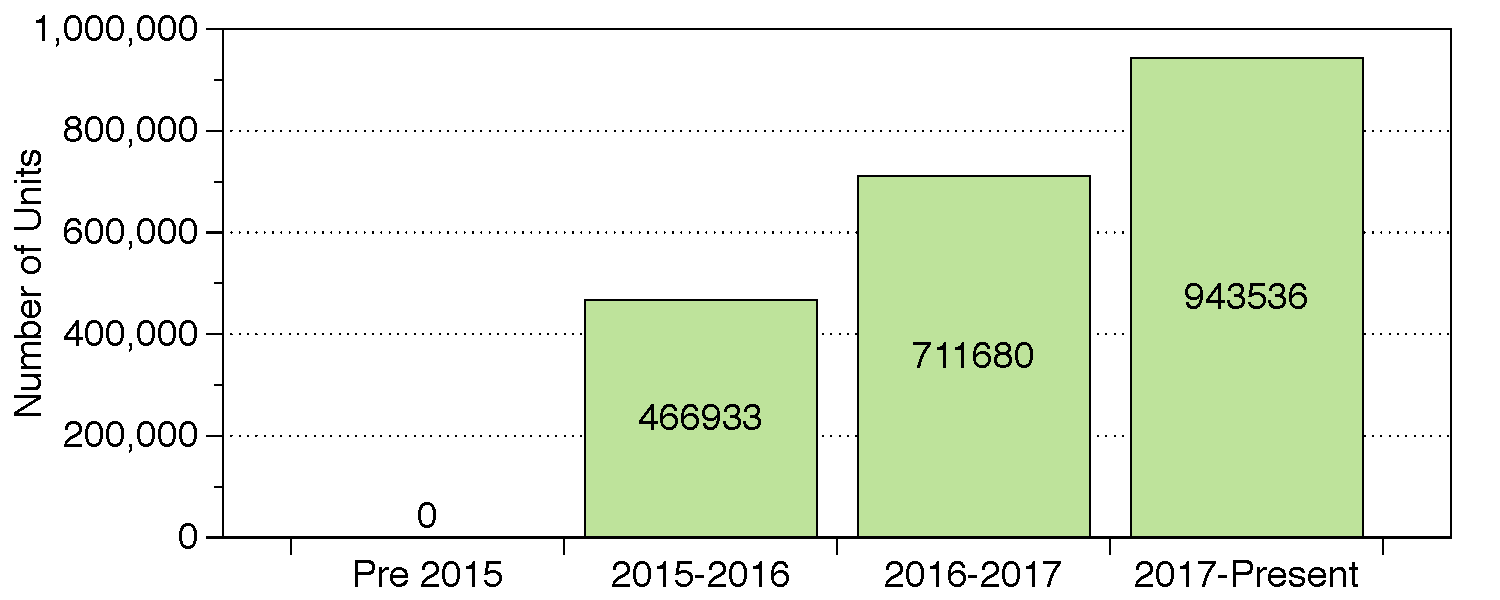
\includegraphics[trim=0 0 0 -10, clip, width=1.0\columnwidth]{figs/faa}
  \caption{Rapidly growing interest in UAVs. Data mined from FAA vehicle registration. The number of FAA registrations increased by 2X over the past two years, and it is rapidly growing. The FAA projects that by 2021 the number will exceed 4M units~\cite{FAA:online}.}
  \label{fig:faa-registrations}
\end{figure}


%\red{What are the big technical problems with drones} \lipsum[1]

The growth and significance of this emerging domain of autonomous agents call for architects attention. Challenges such as low endurance (how long the drone can last in the air) and small battery capacities for drones demand hardware and system architects' attention. The limited on-board energy budget manifests itself in the limited endurance and range of drones. This can be seen in various off-the-shelf commercial drones where endurance is typically less than 20 minutes, and flight range is about 15 miles~\cite{CSD-Amazon-Drone-patents}. To practically deploy drones, both their endurance and range must be improved. 

%\red{What should architects do here to help with the technical problems and what do they typically require here} \lipsum[1]

In this paper, we investigate and show the role of computing given the endurance and range challenges. For example, we show how a powerful compute subsystem can be deployed to mitigate the problem of limited endurance. The drone's compute subsystem dictates how fast a drone can maneuver, fly, and efficiently finish its mission. Hence, a computing subsystem that takes a long time to do path planning while the drone is hovering in the air, results in the inefficient consumption of energy. Furthermore, a more powerful compute subsystem can lead to more intelligent decision making (e.g., shorter paths to take). It is important to note that enabling intelligence on drones is challenging because of the computational power, size, weight, and cooling limitations.

%\red{Explain HILS and MAVBench goals} \lipsum[1]

To enable research and investigation, the foremost challenge to address is the lack of systematic benchmarks and infrastructure for research. To address this shortcoming, we introduce MAVBench, the first of its kind, a platform for the holistic evaluation of aerial agents, involving a closed-loop simulation framework and a benchmark suite. MAVBench facilitates the integrated study of performance and energy efficiency of not only the compute subsystem in isolation but also the compute subsystem's dynamic and runtime interactions with the simulated micro-aerial vehicle (MAV) as a whole.

%\red{Deep dive into the simulator -- one para} \lipsum[1]

The goals of MAVBench, which builds on top of AirSim~\cite{Airsim_paper}, are to faithfully capture all the interactions a real MAV encounters in the field and to ensure reproducible runs across experiments, starting from the software layers down to the hardware layers. Our simulation setup uses a hardware-in-the-loop configuration that can enable hardware and software architects to perform co-design studies to optimize system performance by considering the entire vertical application stack running on top of it, which includes the Robotics Operating System (ROS) and complete applications. It reports a variety of quality-of-flight (QoF) metrics, such as the performance, power consumption, and trajectory statistics of the drone.

%\red{Explain what MAVBench contains and why it is useful} \lipsum[1]
MAVBench provides an application suite covering a variety of popular applications of micro aerial vehicles. We constructed five distinct and widely used applications: \bench{Scanning}, \bench{Package Delivery}, \bench{Aerial Photography}, \bench{3D Mapping} and \bench{Search and Rescue.} MAVBench applications are whole, comprised of holistic end-to-end application dataflows found in a typical real world drone application. These applications' dataflows are comprised of several state-of-the-art computational kernels, such as object detection~\cite{yolo16,hog}, occupancy map generation~\cite{octomap}, motion planning~\cite{ompl}, localization~\cite{orbslam2,vins-mono}, which we integrated together to create complete applications. MAVBench has the ability to ``plug and play'' different computational kernels to study trade-offs for the same task.

%\red{What are some of the research observations we make} \lipsum[1]

MAVBench enables us to investigate, understand and quantify the power and performance demands of typical MAV applications from the underlying compute subsystem. More specifically, it allows us to answer a very fundamental question: \emph{what is the role of computing in autonomous MAVs?} 

We quantitatively demonstrate via simulations and measurements that compute has a significant impact on how efficiently the drone uses its energy while flying, affecting mission times and overall energy consumption. An off-the-shelf MAV, such as the DJI~Matrice~\cite{dji-matrice} or \solo~\cite{solo3DR}, consumes between 300~W to 400~W for its rotors, as much power as a typical data center server, with an average endurance that is typically less than 20 minutes. Compute on average consumes less than 5\% of that total system power.  A state-of-the-art compute platform like the Nvidia TX2 consumes about 10~W on average. However, the compute performed onboard by the TX2 can affect flight mission time by as much as 2X. We conduct frequency and core scaling experiments on the TX2 to demonstrate how the \emph{compute performance affects the drone's velocity, which in turns impacts its mission time, and consequentially the drone's total system energy consumption.}

Taking advantage of our platform, we provide three case studies targeting performance, energy and reliability. The performance case study examines a sensor-cloud architecture for drones where the computation is distributed across the edge and the cloud. Such an architecture shows a reduction in the drone's overall mission time by as much as 50\% when the cloud support is enabled. The energy case study, targets Octomap~\cite{octomap}, a computationally intensive kernel that is at the heart of some of the MAVBench applications and demonstrates how approximations in its internal representation, and thus compute, can enable safe flight while improving overall energy consumption. Last by not least, our reliability case study investigates the impact of sensor noise on the performance of one of our applications, namely package delivery, showing a performance degradation of up to 90\% while in presence of high depth image noise. All three case studies demonstrate the potential ways in which MAVBench can be used for architecture and systems research. In general, the platform allows a variety of hardware and software (co-)design studies.

%OctoMap generates a volumetric 3D model of its environment that the collision avoidance and motion planning task use to ensure a safe flight. By dynamically adjusting OctoMap's ``resolution'' (i.e., perception) of the environment, we can control the amount of computing performed for a trade off in accuracy. Expediting OctoMap processing leads to faster real-time decision making and max safe velocity. This allows the drone to fly faster and complete its mission with more energy remaining in its battery. 

In summary, we make the following contributions:

\begin{itemize}
    \item We present a closed-loop simulation framework that enables hardware and software architects to perform performance and power optimization studies that are relevant to computer system design and architecture.
    \item We introduce an end-to-end benchmark suite, comprised of several workloads and their corresponding state-of-the-art kernels. These workloads represent popular real-world use cases of MAVs.
    \item We uncover the role of computing and its relationship with flight time and endurance for unmanned MAVs.
    \item We present case studies to concretely explore and emphasize compute's impact on performance, energy and reliability of MAV systems.

\end{itemize}


\begin{comment}


Furthermore, on the road to intersect with the proliferation of drones is the interest in making these aerial systems fully autonomous~\cite{gopalakrishnan2016countermeasures}. There is growing interest in equipping drones with more intelligence using recent advancements in AI and machine learning. One of the primary motivations for adding these capabilities is to eliminate the human in the loop. Human operators are an unreliable source of operation. Over 85\% of general aviation crashes are caused by pilot error~\cite{li2001factors,shkrum1996fatal}.


This paper is an attempt to present an architectural overview of aerial agents, and further provide tools to study them, namely, a simulation platform and a benchmark. In addition, we conduct various case-studies using aforementioned tools, and show invaluable conclusions such tools enable. More concretely, our contributions are three fold:
	  \begin{itemize} 
       \item A closed-loops end-to-end simulation environment as a necessity to probe into the extra-system (system/environment) and intra-system interactions. Case studies are further presented to show how ignoring such interactions can be detrimental to design and development of aerial systems and hence platforms without such probing capabilities should be abandoned (section 3). 
      \item Mav-bench: A new and diverse benchmark suit targeting aerial computing enabling architects for characterization/design and development of aerial agents (section 4 and 5).
	\item  unraveling the non-traditional compute/energy relationship existing for such systems. Concrete ways in which compute can affect the overall systems energy and in-turn agents mission success is studied and presented (section 6)
      \end{itemize}
   
\end{comment}

The rest of the paper is organized as follows. 
%\Sec{sec:background} gives background on UAVs and MAVs that is relevant to this paper. 
~\Sec{sec:background} provides basic background about Micro Aerial vehicles, the reasons for their prominence amongst UAVs, and the challenges system designers face.  \Sec{sec:simulation} describes the MAVBench closed-loop simulation platform. \Sec{sec:mavbench} introduces the MAVBench benchmark suite and describes the computational kernels and full-system stack it implements. \Sec{sec:char} uses MAVBench to uncover an interesting relationship between compute and the MAV's total system energy consumption. \Sec{sec:case-study} presents three case studies further examining the impact of compute stack on performance, energy and reliability of MAV systems. \Sec{sec:related} discusses related work, and \Sec{sec:conclusion} summarizes and concludes the paper.
       
\section{Background}
\label{sec:background}

We provide a brief background about unmanned aerial vehicles (UAVs). 
%In \Sec{sec:uav}, we present the lay of the land, discussing the different types of UAV tiers. 
In \Sec{sec:mav}, we discuss the most ubiquitous and growing segment of UAVs, i.e., Micro Aerial Vehicles (MAVs) and its different flight-wing types. In  \Sec{sec:constraints}, we present the overall system level constraints facing MAVs.

\begin{comment}
\subsection{Unmanned Aerial Vehicle (UAV) Tiers}
\label{sec:uav}

There is no single established standard to categorize all drones. However, certain high-level characteristics such size as weight, and range, all of which ultimately determine the drone use case, can be used as the base for such clustering. Table~\ref{nato-classification-drones} shows one such proposed classification guide provided by NATO. This classification allows drones to be specified based on the altitude and range which missions require.

Drones, otherwise known as Unmanned Aerial Vehicles (UAVs), initially emerged as military weapons to be mainly deployed for missions in which having a human pilot will be a disadvantage~\cite{rs}. It is not until recently that there has been a significant proliferation of Micro Aerial Vehicles (MAV) for civilian applications, such as crop surveying, industrial fault detection, mapping, surveillance and aerial photography. 


\begin{table}[t!]
\vspace{5pt}
\centering
\caption{UAVs by NATO Joint Air Competence Power~\cite{nato-uav-classification}.}
\label{nato-classification-drones}
\resizebox{\columnwidth}{!}{
\begin{tabular}{|c|c|c|c|}
\hline
Category                                                              & Weight (kg) & Altitude (ft) & Mission Radius (km) \\ \hline\hline
Micro                                                                 & \textless2                                             & \textless200                                                                    & 5                                                                           \\ \hline
Mini                                                                  & (2-20)                                                 & (200- 3000)                                                                     & 25                                                                          \\ \hline
Small                                                                 & (20-150)                                               & (3000-5000)                                                                    & 50                                                                          \\ \hline
Tactical                                                              & (150-600)                                              & (5000-10000)                                                                    & 2000                                                                        \\ \hline
Combat & \textgreater600                                        & \textgreater10000                                                               & Unlimited                                                                   \\ \hline
\end{tabular}
}
\end{table}


\begin{comment}
\begin{table}[]
\centering
\caption{Classification based on Size}
\label{my-label}
\begin{tabular}{|l|l|}
\hline
\textbf{Size} & \textbf{Value}  \\ \hline
Very Small    & 30 to 50 cm     \\ \hline
Small         & 50 to 2 m       \\ \hline
Medium        & 5 to 10 m       \\ \hline
Large         & \textgreater10m \\ \hline
\end{tabular}
\end{table}
\begin{table}[]
\centering
\caption{Classification of UAV based on Range and Endurance}
\label{my-label}
\begin{tabular}{|l|l|l|}
\hline
\textbf{Class}   & \textbf{Range} & \textbf{Endurance}    \\ \hline
Very Close Range & 5 Km           & 20-45 min             \\ \hline
Close Range      & 50 Km          & 1 to 6 Hours          \\ \hline
Short Range      & 150 Km         & 8 to 12 Hours         \\ \hline
Mid Range UAV    & 650 Km         & 12 to 36 Hours        \\ \hline
Endurance UAV    & 300 Km         & \textgreater 36 Hours \\ \hline
\end{tabular}
\end{table}
\end{comment}

\subsection{Micro Aerial Vehicles (MAV)}
\label{sec:mav}
There is no single established standard to categorize all drones. However, typically, a UAV is classified as a ``Micro UAV'' if its weight is less than 2~\si{\kilo\gram}, and it operates within a radius of 5~\si{\kilo\meter}. MAVs' small size increases their accessibility and affordability by shortening their ``development and deployment time,'' as well as reducing the cost of ``prototyping and manufacturing''~\cite{Zhang2017207}. Furthermore, their small size coupled with their ability to move flexibly empowers them with the agility and maneuverability necessary for various applications, such as sports photography, indoor mapping, surveillance, etc.

MAVs come in different shapes and sizes. A key distinction is their wing type. On one end of the spectrum, MAVs have fixed wings. On the other end, MAVs have rotor wings. Fixed wing MAVs, as their names suggest, have fixed winged airframe. Their wing structure is deployed for taking-off, navigation, and landing. These MAVs typically require (small) runways for taking-off and landing. Due to the aerodynamics of their wings, they are capable of gliding in the air, which improves their ``endurance'' (i.e., how long they last in the air).

Rotor wing MAVs are becoming the dominant kind. They take off vertically, land vertically, and move with more agility compared to their fixed-wing counterparts. They do not require constant forward airflow movement over their wings from external sources since they generate their own thrust using rotors. Such capabilities enhance their benefits in constrained environments, especially indoors, such as in buildings and warehouses where there are many tight spaces and corners.

Although MAVs enjoy the aforementioned advantages, their complex mechanical (rotors/payload etc) and electrical subsystem (battery, processors) limit their endurance, and as such present unique challenges for system architects and engineers.

\begin{figure}[t!]
\centering
    \begin{subfigure}{.49\columnwidth}
    \centering
    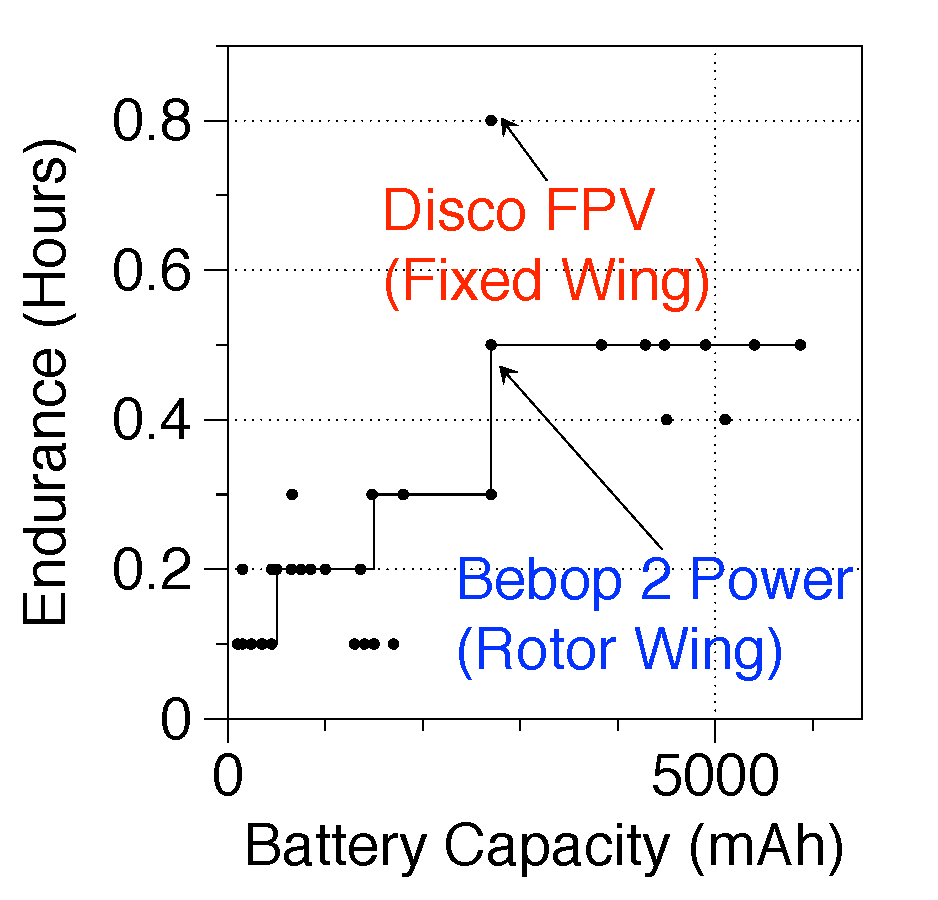
\includegraphics[trim=0 0 0 0, clip, width=0.9\columnwidth]{figs/Battery_Capacity_vs_Endurance_plot}
   \vspace{-5pt}
   \caption{Flight endurance time plotted against total battery capacity.}
    \label{fig:battery_capacity_vs_endurance}
    \end{subfigure}
    \hfill
    \begin{subfigure}{.49\columnwidth}
    \centering	
    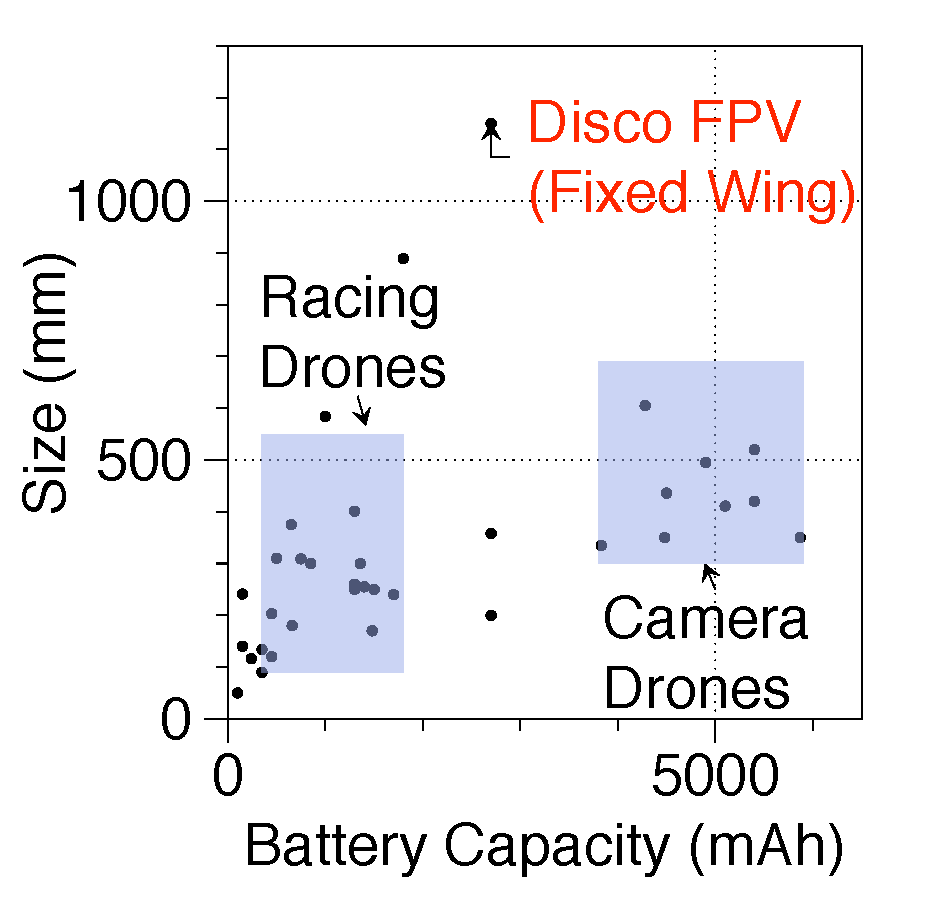
\includegraphics[trim=0 0 0 0, clip, width=0.9\columnwidth]{figs/Size_vs_Battery_Capacity}
    \vspace{-5pt}
    \caption{Drone size plotted against total battery capacity.}
    \label{fig:battery_capacity_vs_size}
    \end{subfigure}
\caption{MAVs based on battery capacity and size. Endurance is important for MAVs to be useful in the real-world. However, their small size limits the amount of on-board battery capacity.}
\label{fig:tradeoff}
\end{figure}

\begin{comment}

\subsection{rotor-based Micro Aerial Vehicles: UAV of choice}
%Among the aforementioned categories, rotor-based Micro aerial vehicle have an outburst of attention in recent years. This section elaborates how their rotor-based flight mechanism and smaller size can explain such a trend.

\textit{rotor based flight mechanism:} Using their flight mechanism, one can classify UAVs to fixed wing, flapping wing, or rotary wing. Though fixed-wings "simpler structure and more efficient aerodynamics provide the advantage of longer flight"(http://www.uavinsider.com/rotary-wing-vs-fixed-wing-uavs/),  the aircrafts with rotors are capable of "
%vertically taking off and landing, fixed-point hovering, flying
at low level altitude, and great stability and maneuverability."~\cite{Development-of-a-Micro-Aerial-Vehicle}. 

\textit{small size:} MAVS are aircrafts of size less than 15 cm length, width, or height and weigh less than 100 g. Such a small size have increased accessibility and affordibily of such systems by shortening the "development and deployment time", and reducing the cost for "prototyping and manufacturing", ~\cite{Rugged Embedded Systems 1st Edition book}. 
In addition, the combination of the small size and the hovering capability of the rotors provide these systems with the agility and  maneuverability necessary for various applications such as sports photography, indoor mapping, surveillance and etc.
\end{comment}

%Micro-Aerial Vehicles(MAV) comes in different shapes and sizes. On one end of the spectrum, MAV have fixed wing. On the other end, we have rotor based. Both these type of MAV can have electric motors or internal combustion engine as the propulsion system. The choice of propulsion system has a direct impact on the range and endurance of the MAV. There are also hybrid MAVs which uses both electric and internal combustion engine for propulsion. 

\begin{comment}
\begin{table}
\centering
\resizebox{\columnwidth}{!}{%
\caption{Drone categories.}
\label{tab:drones}
\begin{tabular}{|l|l|l|l|l|}
\hline
Category          & weight & range(km) & endurance(h) & altitude(h)     \\ \hline\hline
Micro       \textless2      &  \textless1      &           & 5-30 min     & \textless330 \\ \hline
Mini              &  \textless1 &           & 1-2          &              \\ \hline
Small             &    \textless13.5    &           &              &              \\ \hline
Light/ultra Light &     \textless242   &           &              &              \\ \hline
Normal            &   \textless4332     &           &              &              \\ \hline
Large             &     \textless4332   &           &              &              \\ \hline
\end{tabular}
}
\end{table}
\end{comment}

\begin{comment}
\subsection{Drone Platforms}
\label{ssec:drone-arch}
\begin{table}[]
\centering
\caption{Drone tiers: this table will contain high level ideas about drones from the pure functionality level, i.e. no system design perspective. e.g frame size, flight time, max speed, avg payload, max payload}

\label{my-label}
\begin{tabular}{|l|l|}
\hline
Drone Type & Frame size {[}mm{]} \\ \hline
Nano       & 80-100              \\ \hline
Micro      & 90-180 mm           \\ \hline
Mini       & 150-300             \\ \hline
\end{tabular}
\end{table}
Table~\ref{tab:drone-platforms}
\begin{table*}[t!]
\centering
\caption{Drone platform characteristics. pick a drone from different tiers and introduce the specs (from system perspective)}
\label{tab:drone-platforms}
\begin{tabular}{ |p{3cm}||p{3cm}|p{3cm}|p{3cm}|  }
 \hline
 Name     or Area Name& A nano drone name & a micro drone name & a mini drone name \\
 \hline
Power   & AF    &AFG&   004\\
Flight-time &   AX  & ALA   &248\\
Battery &AL & ALB&  008\\
FMU    &DZ & DZA&  012\\
Payload &   AS  & ASM&016\\
... & AD  & AND   &020\\
Companion computer & AO  & AGO&024\\
 \hline
\end{tabular}
\end{table*}
\end{comment}

\begin{comment}
\subsection{System Architecture old}
\label{ssec:drone-arch}

\red{in this section we explain the general architecture of a drone, since all the drones generally follow the same subsystem design. this is basically about the system architecture that is used by all the drones. explain the components within and how they interact etc.}

A typical autonomous MAV is equipped with an on-board computer, a flight controller, a collection of sensors, and a set of mechanical components including propellers and motors.

\paragraph{On-board Computer} A drone requires an on-board computer for autonomous flight. This on-board computer is responsible for high-level flight control and for computations that are not directly related to flight such as object detection or machine learning.

\paragraph{Flight controller} The flight controller is a microcontroller that handles a variety of low-level flight-related tasks. For example, it stabilizes the drone during flight, logs flight data, and controls the drone's orientation and speed to move it in the fashion specified by the on-board computer.

\paragraph{Sensors} Drones have the capability of gathering a rich set of sensory data, and the sensors they are equipped with will vary depending on the application that they are intended for. At minimum, however, a typical autonomous drone will be equipped with a sensor, such as an inertial measurement unit, that detects orientation, a sensor, such as a barometer or ultrasonic sensor, that detects altitude, and a sensor, such as a GPS receiver or optical flow camera, that detects position. There are many other possible sensors that may be attached to drones such as LIDAR sensors for 3-D mapping, cameras for photography, or even multispectral sensors for the purpose of monitoring crop health.

\paragraph{Other} In addition to sensors and processors, drones are composed of mechanical components such as motors, propellers, and frames.

\begin{figure}[h]
\centering
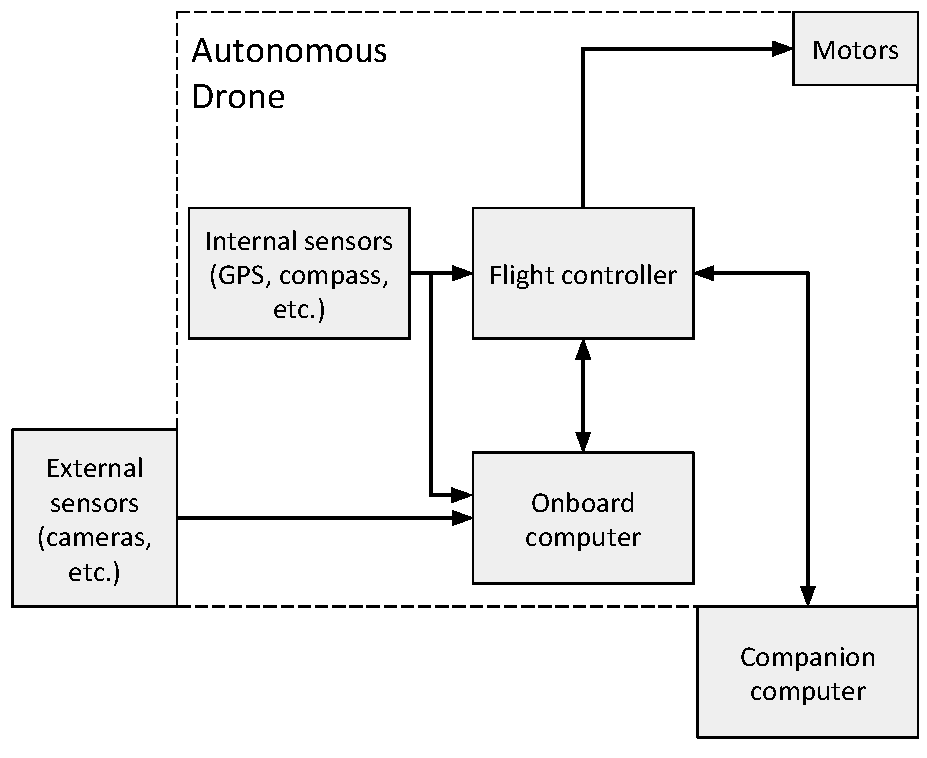
\includegraphics[width=\linewidth]{figs/drone-arch}
\caption{Architectural overview of our drone platform.}
\label{fig:dronearch}
\end{figure}
\end{comment}

\subsection{MAV Constraints}
\label{sec:constraints}

MAVs are tightly constrained on their resources. These constraints typically have to do with the limitations in the mechanical subsystems (rotors/payload size etc.) and the electrical subsystem (battery/processor etc.). For example, in package delivery, the payload size (i.e., the package) affects the mechanical subsystem, requiring more thrust from the rotors and this, in turn, affects the electrical subsystem by demanding more energy from the battery source. Comprehending these constraints is crucial to understand how to optimize the system. The biggest of the constraints as they relate to computer system design are performance and energy.

%At the high level, application (package delivery) requirements (lifting certain payload size for a certain range) turns into mechanical (rotors/motors thrust) and energy source (LIPO battery capacities) constraints. In turn, such constraints manifest themselves as performance and power constraints for architects to deal with. In this section we iterate over such constraints:

\paragraph{Performance Constraints:} MAVs are required to meet various real-time constraints. For example, a drone flying at a high speed looking for an object requires fast detection kernels. Such a task is challenging in nature for large-sized drones that are capable of carrying high-end computing systems, and they are virtually impossible on smaller sized MAVs. Hence, the stringent real-time requirements dictate the type of compute engines that can be put on these MAVs.

\paragraph{Energy Constraints:} The amount of battery capacity on board plays an important role in the type of applications MAVs can perform. Battery capacity has a direct correlation with the endurance of these vehicles. To understand this relationship, we show the most popular MAVs available in the market and compare their battery capacity to their endurance. As \Fig{fig:battery_capacity_vs_endurance} shows, higher battery capacity translates to higher endurance. We see a step function trend, i.e., for classes of MAVs that has similar battery capacity, they have similar endurance. On top of this observation, we also see that for the same battery capacity, a fixed wing has longer endurance compared to rotor based MAVs. For instance, in \Fig{fig:battery_capacity_vs_endurance}, we see that the Disco FPV (Fixed wing) has higher endurance compared to the Bebop 2 Power (Rotor wing) even though they have a similar amount of battery capacity.
Note that the size of MAV also has a correlation with battery capacity as shown in \Fig{fig:battery_capacity_vs_size}. 
%\red{I don't see how this discussion is relavant at all to architects. There should be at least one pointer we'll that connects this paragraph to architects}

\begin{comment}
\begin{figure}[t!]
\centering
\tabskip=0pt
    \begin{subfigure}{\columnwidth}
    \centering
    \vspace{0.1in}
    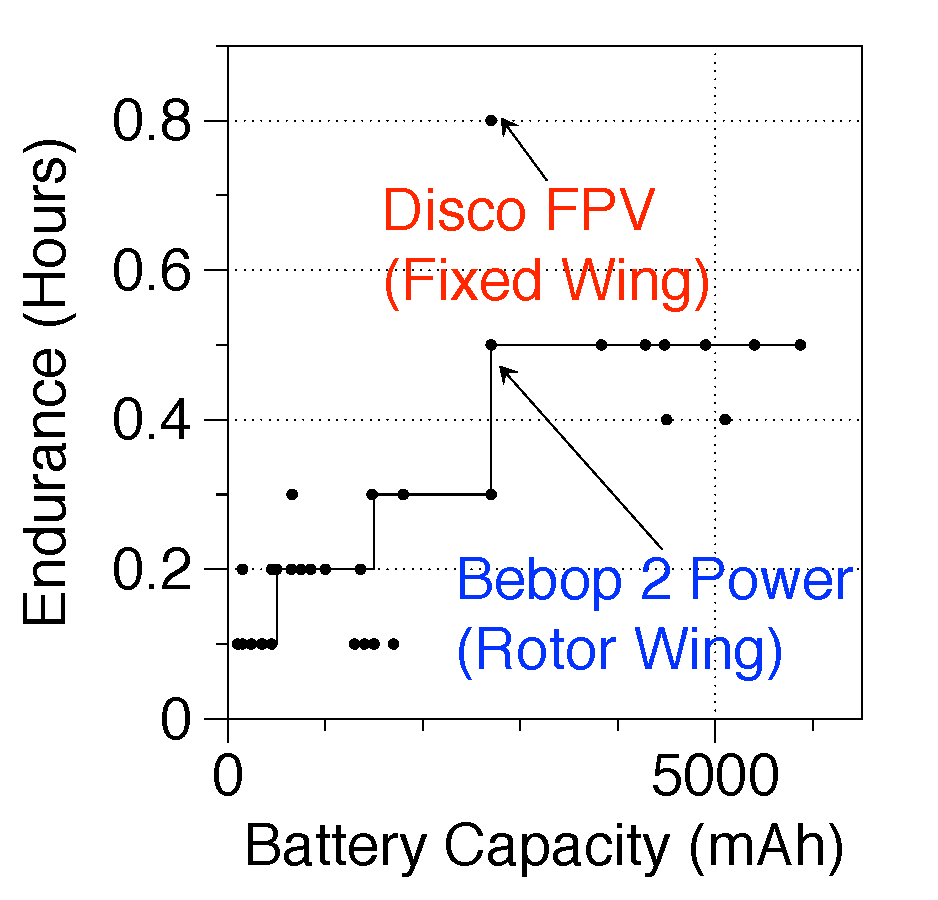
\includegraphics[trim=0 0 0 0, clip, width=.9\columnwidth]{figs/Battery_Capacity_vs_Endurance_plot}
    \caption{Endurance versus battery capacity.}
    \label{fig:battery_capacity_vs_endurance}
    \end{subfigure}
    \begin{subfigure}{\columnwidth}
    \centering
    \vspace{0.1in}
    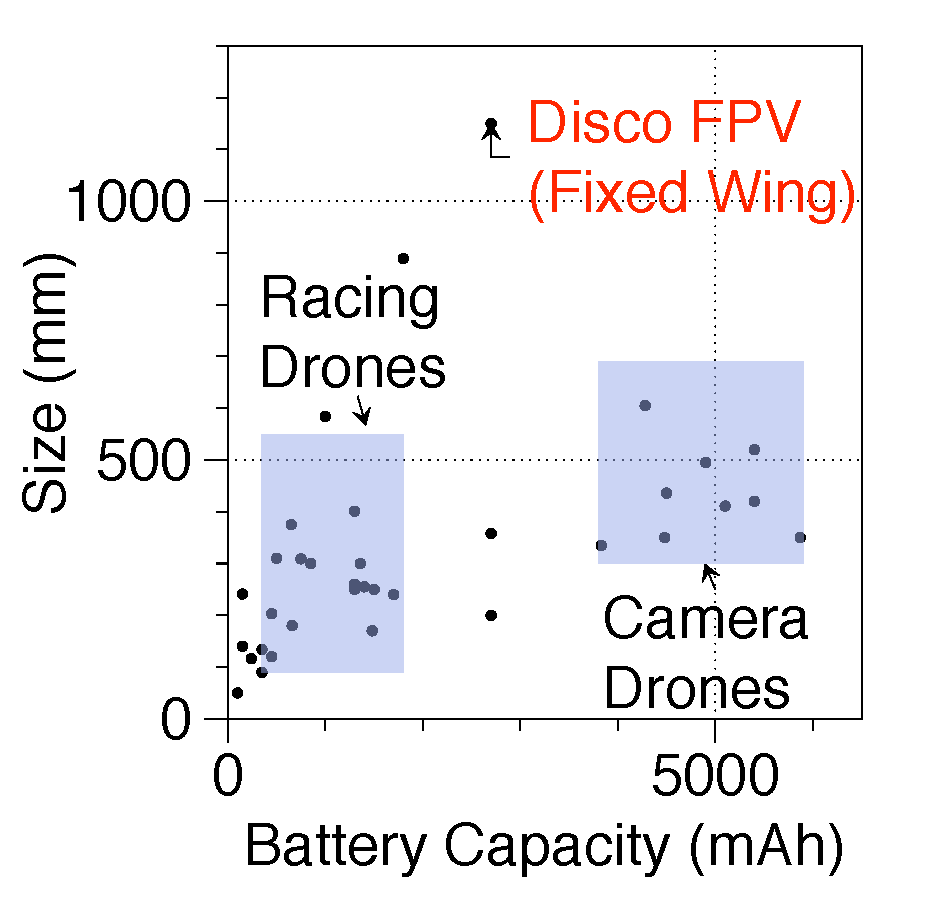
\includegraphics[trim=0 0 0 0, clip, width=.9\columnwidth]{figs/Size_vs_Battery_Capacity}
    \caption{Size versus battery capacity.}
    \label{fig:battery_capacity_vs_size}
    \end{subfigure}
\caption{MAVs based on battery capacity and size. Endurance is important for MAVs to be useful in the real-world. However, their small size limits the amount of on-board battery capacity.}
\label{fig:tradeoff}
\end{figure}
\end{comment}
%\red{I don't think we need the following two constraints. They are not relavant to architects, or if they are, it's hard to argue. also get rid of the figure that comes with it}
%\paragraph{Size:}The Size of MAV plays an important role in selection of mechanical and electrical subsystem. \Fig{fig:battery_capacity_vs_size} shows the distribution of size of MAVs and the battery capacity. MAVs deployed for aerial photography/surveying have higher battery capacity for their sizes. The racing MAVs are much smaller in size compared to camera MAVs but have more battery capacity for their size. However, racing MAVs typically have lower flight times in the order five to ten minutes because all the energy is spent generating higher thrusts.

%\red{this paragraph is confusing. where are the aerial photography/scanning drones in the figure. Are they camera drones? also it doesn't seem like we are discussing size constraints, but rather the implications of picking a size. also I think we should get rid of this or combine it with weight and imply the }

%\paragraph{Weight:} MAV weight, inclusive of its payload weight, can also have a significant impact on its endurance. Higher payload puts stress on the mechanical subsystems requiring more thrust to be generated by the rotors for hovering and maneuvering. This significantly reduces the endurance of MAVs. For instance, it has been shown that adding a payload of approximately 1.3~\si{\kilo\gram} reduces flight endurance by 4X~\cite{hasan2016sensorcloud}.


%Since most of the above-mentioned constraints either leads to performance bottlenecks in compute or energy consumption, opening up interesting avenues for research in computer architecture.\red{<- wording doesnt make sense. I also see the connection to compute architects.} To address these problems, computer architects need tools that extend beyond traditional simulators. 

%The aforementioned constraints opens up interesting avenues for research in computer architecture. To address these problems, computer architects need tools that extend beyond traditional simulators.



%Weight constraint is essential to the functioning of the aircrafts such as taking-off and stability. However, it has system implications. For example, it can throttle the system's thermal power budget since the added weight associated with introducing a fan might not be a possibility
%As was dicussed , the need to be mobile with high exploratory capacities constraints aerial agents to their amount of energy on board. (possibly cite one platform with flight time). As a result, longer flight time due to lower system performance can cause system to run out of energy and hence fail its mission. Performance improvements such as decreasing the decision making time (while drone hovers\footnote{one can think of this analogous to reduction of processor idle times}), or increasing decisions optimality (e.g. shorter paths to take while navigating) allows such systems to stay within energy budget. 

%\begin{figure}[t!]
%\centering
%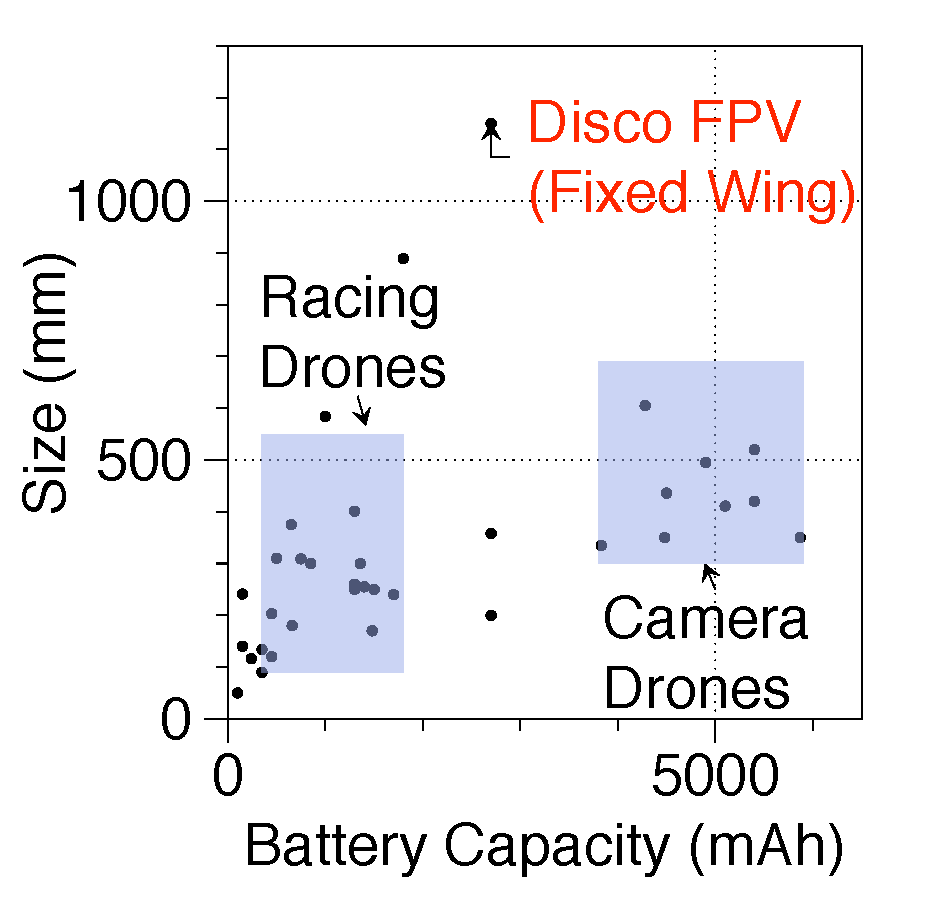
\includegraphics[width=0.5\columnwidth]{figs/Size_vs_Battery_Capacity}
%\vspace{-.4ex}
%\caption{ }
%\vspace{-3ex}
%\label{fig:1}
%\end{figure}

%\begin{figure}[t!]
%\centering
%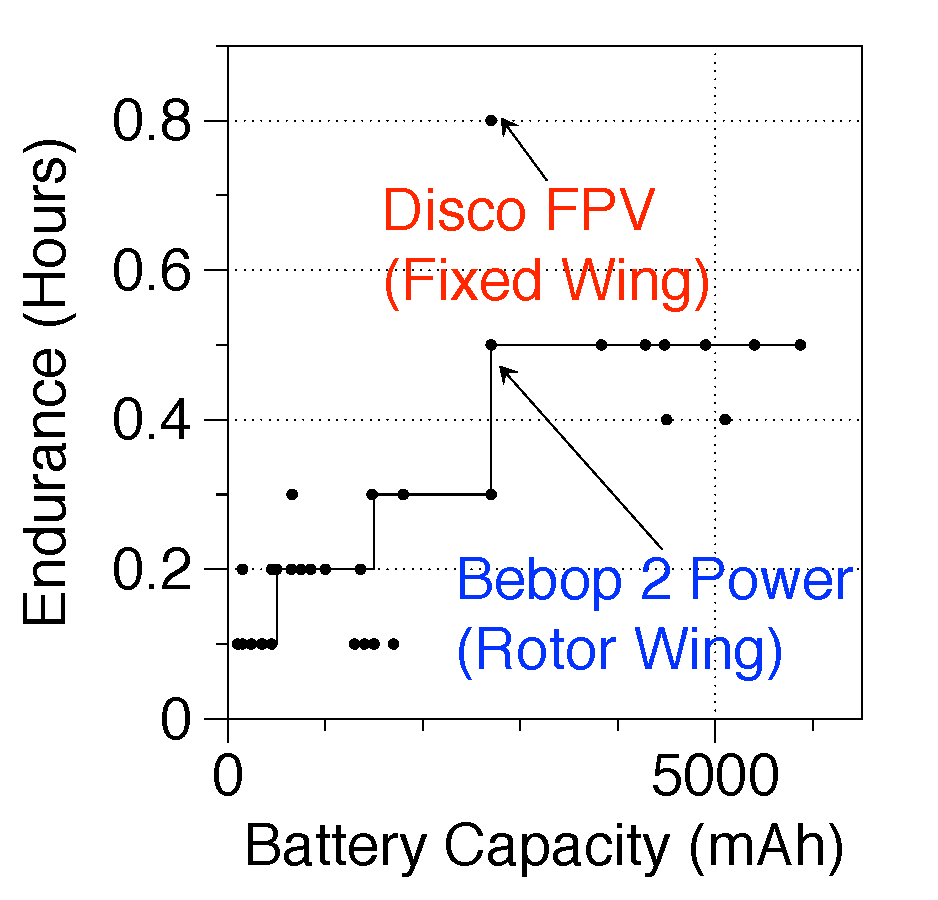
\includegraphics[width=0.5\columnwidth]{figs/Battery_Capacity_vs_Endurance_plot}
%\vspace{-.4ex}
%\caption{ }
%\vspace{-3ex}
%\label{fig:1}
%\end{figure}


\begin{comment}
\red{here we explain the power and performance characteristics of drones from the data that is presented in the table. the goal is to provide intuition about what is going on in terms of power consumption and what is the peak performance of the native platform...}

There are multiple factors that affect drone flight performance. These include energy constraints, maximum payload size, total weight, and computing capability.

\paragraph{Energy Constraints} A drone's energy constraints include its battery lifetime and the power consumption of its components. Battery lifetime is of the utmost relevance to a drone's performance because it limits a drone's maximum lifetime, which in turn restricts the maximum range to which a drone can fly. If battery lifetime is low, then package delivery drones, for example, may not be able to service rural areas that are far from flight stations. Companies may also have to build expensive recharging stations where drones can stop mid-route in order to extend their range.

\paragraph{Payload Size} Drones may be required to carry external payloads during their flights. Package delivery drones are the most obvious example, but search and rescue drones can also carry payloads in order to leave survivors they discover with food, water, and other survival materials before emergency responders can arrive. Although large payloads may be desirable, they can also be disadvantageous to a drone's flight performance. Large payloads will reduce a drone's stability, which may make it difficult for it to fly in anything other can calm weather, and they will increase a drone's weight and thus the total power consumed by motors in flight.

\paragraph{Total Weight} A drone's total weight is heavily correlated with its power consumption, which, as mentioned above, can have a dramatic effect on a drone's performance. The heaviest component of a drone is usually the battery which must be carefully selected so as to find the optimum trade-off between battery capacity and battery weight. The heavier a drone's battery, the more energy it can provide for flight, but the more power it takes be lifted off the ground.

\paragraph{Compute} For drones to be fully autonomous, they must be able to process data about their surroundings at high frame rates. For computationally intensive operations like object detection, powerful CPUs and GPUs may be required.

\paragraph{Communication} Autonomous drones may communicate with ground stations or other drones while in flight. As long as they are able to maintain communication, they can offload computations or mission tasks to off-board components which can improve their performance. In certain environments, however, communication may be unreliable and so autonomous drones must still be able to complete their tasks when they lose communication with off-board components, even if their performance drops as a result.

\paragraph{Speed} Drones that fly fast must be able to process incoming information much more quickly than those that fly more slowly in order, for example, to avoid collisions. Therefore, fast-flying drones require more powerful on-board computers to achieve safe autonomous flight. They will also require more advanced IMUs and flight controllers in order to maintain stability at high speeds.
\end{comment}
%\paragraph{Computational capability} Limits the tasks that a drone can be expected to do.

%\paragraph{Power consumption} Limits the time that a drone has to complete its tasks

%\paragraph{Others} Other factors affecting drone performance that can be quantified by our benchmarking suite or model.

%\externaldocument{./../tex/MAVBench.tex}

\section{Closed-loop Simulation}
\label{sec:simulation}
\setstcolor{red}

We discuss a closed-loop simulation environment for simulating and studying MAVs. In \Sec{sec:components}, we describe the components of a MAV, how they interact and why the intra- and inter-system interactions are important to capture. In \Sec{sec:setup}, we show how our setup captures these components and their interactions in a closed-loop setup. In \Sec{sec:energy}, we describe how the simulator models energy consumption, in addition to the functional and performance data described in the earlier section. In \Sec{sec:knobs}, we describe the knobs that our simulator supports to enable exploratory studies, and in \Sec{sec:accuracy}, we describe the limitations of our current setup and opportunities for future enhancements. 
 
\begin{figure}[t!]
\centering
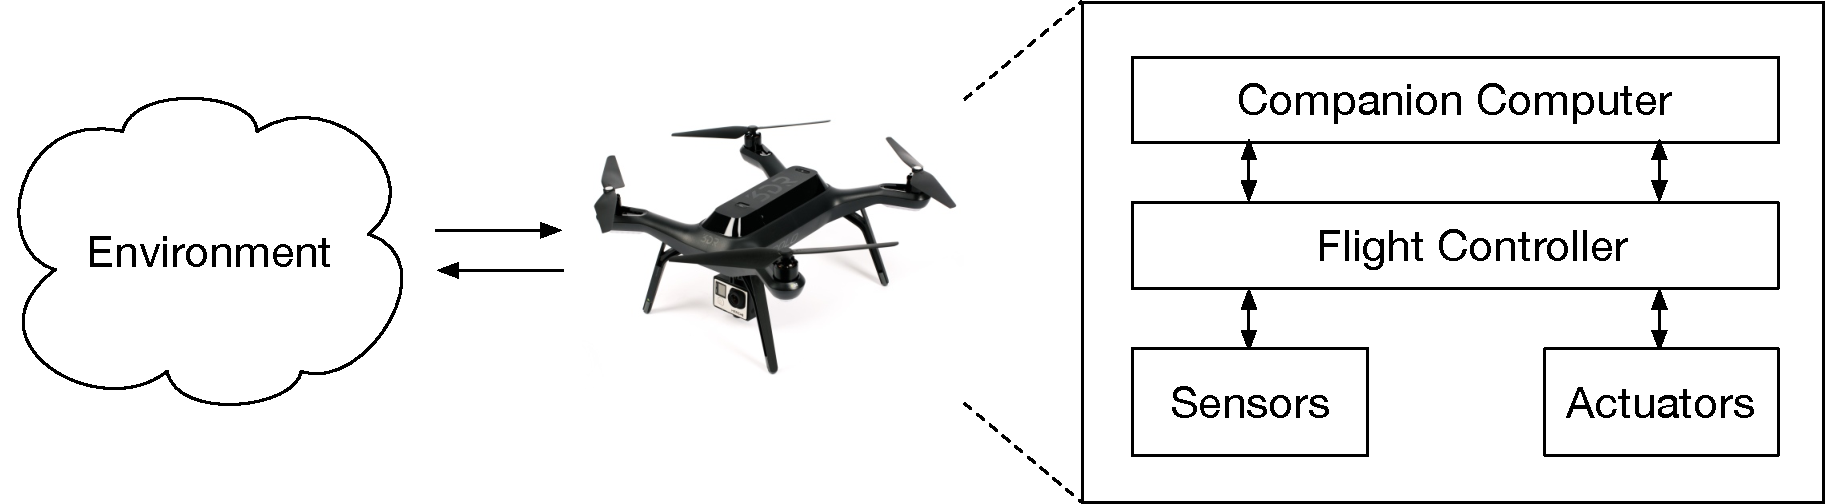
\includegraphics[trim=0 0 0 -25, clip, width=0.9\linewidth]{figs/Aerial_agent_3}
\caption{Closed-loop data flow in a MAV. Information flows from sensors collecting environment data into the MAV's compute system, down into the actuators and back to the environment.}
\label{fig:Aerial_agent_data_flow}
\end{figure}

\subsection{MAV System Components Dissected}
\label{sec:components}

Closed-loop operation is an integral component of autonomous MAVs. In such systems, the data flows in a (closed) loop, starting from the environment, going through the MAV and back to the environment as shown in \Fig{fig:Aerial_agent_data_flow}. The process involves sensing the environment (Sensors), interpreting it and making decisions (Compute), and finally navigating within or modifying the environment (Actuators) in a loop. 

\paragraph{Sensors:} Sensors are responsible for capturing the state associated with the agent and its surrounding environment. 
To enable intelligent flights, MAVs must be equipped with a rich set of sensors capable of gathering various forms of data such as depth, position, and orientation. For example, \mbox{RGB-D} cameras can be utilized for determining obstacle distances and positions. The number and the type of sensors are highly dependent on the workload requirements and the compute capability of on board processors for their interpretations.


%\textbf{Perception/Control:} A flight controller and a companion computer provide the compute power for high-level and low-level functions such as object detection and rotor controls. 
\paragraph{Flight Controller (Compute):} The flight controller (FC) is an autopilot system responsible for the MAV's stabilization and conversion of high-level to low-level actuation commands. 
While they themselves come with basic sensors, such as gyroscopes and accelerometers, they are also used as a hub for incoming data from other sensors such as GPS, sonar, etc. For command conversions, FCs take high-level flight commands such as``take-off" and lower them to a series of instructions understandable by actuators such as rotors. FCs use light-weight processors such as the ARM Cortex-M3 32-bit RISC core for the aforementioned tasks.    
 
\paragraph{Companion Computer (Compute):} The companion computer is a powerful compute unit (compared to the FC) that is responsible for the processing of the high level, computationally intensive tasks such as vision processing. Not all MAVs come equipped with companion computers, rather these are typically an add-on option for more processing. NVIDIA's TX2 is a representative example with significantly more compute capability than an FC.

{\paragraph{Actuators:} Actuators allow agents to react to their surroundings and further modify them. They range anywhere from rather simple rotors to robotic arms capable of grasping and lifting objects. Similar to sensors, their type and number is a function of the workload and processing power on board.

\begin{comment}
\subsection{Simulator requirements}
As the system architecture in section III reveals, data flows in a loop for robotic applications, i.e. starting from environment and its sensing to perception, from perception to actuation and back to the environment where its ready to be sensed again. Aerial computing architectural analysis/synthesis demands fast end-to-end simulator, capable of mimicking this closed-loop flow and capturing the interactions across layers. In this section 
%, such features ensure problem identification and solution verification feasibility, and hence allowing simulators to fulfill their role (refer to the other paper).
we discuss how absence/presence of these conditions have architectural ripples. Since simulator design is a never ending battle between accuracy and speed, we analyze the space using these two lenses.


\textit{system/env interactions (Accuracy Impact):} Lacking end-to-end simulation capabilities deprives researcher of design opportunities system/environment interaction consideration provides. In addition, forgoing these interactions can also lead to bottleneck misidentification ,and hence over optimizations. 

(possibly studying the affect of obstacle density on motion planning processing time (and frequency) and deciding whether an accelerator is necessary or not (depending on the env)

\textit{Intra system interactions (Accuracy Impact):} 
Lacking end-to-end inspection can mean having to study application kernels in isolation and hence overlooking the necessary analysis of inter kernels interactions and a design synthesis around it.
examples: 
(1)running slam and object detection and slower than both. But, we gpu zero sharing (for images), we might be able to improve performance.
(2) impact of having bigger caches on delivery last phase (when detection is running. We might be able to model this by lowering the octomap resolution so it'll take less space in the caches)
(3) cache pollution, branch prediction interference.  
//the example need to be 
environment independent, but rather application dependent
   
\textit{speed Impact:}
Wanting to capture above interactions, and given the long mission times (throw some numbers) and irregularity of the environment causing application phases changes, fast simulators are necessary. pure cycle accurate simulators are inviable since it takes ... time to .... 

We believe that a hybrid solution where real embedded-systems, placed in the loop (HIL style) for bottle-neck identification, augmented with an fpga or cycle accurate simulator for testing new ideas is winner solution. 
\end{comment}


\subsection{Simulation Setup}
\label{sec:setup}

We present how our setup, shown in \Fig{fig:end-to-end}, maps to the various components corresponding to a MAV's operation.

\begin{figure}[t!]
\centering
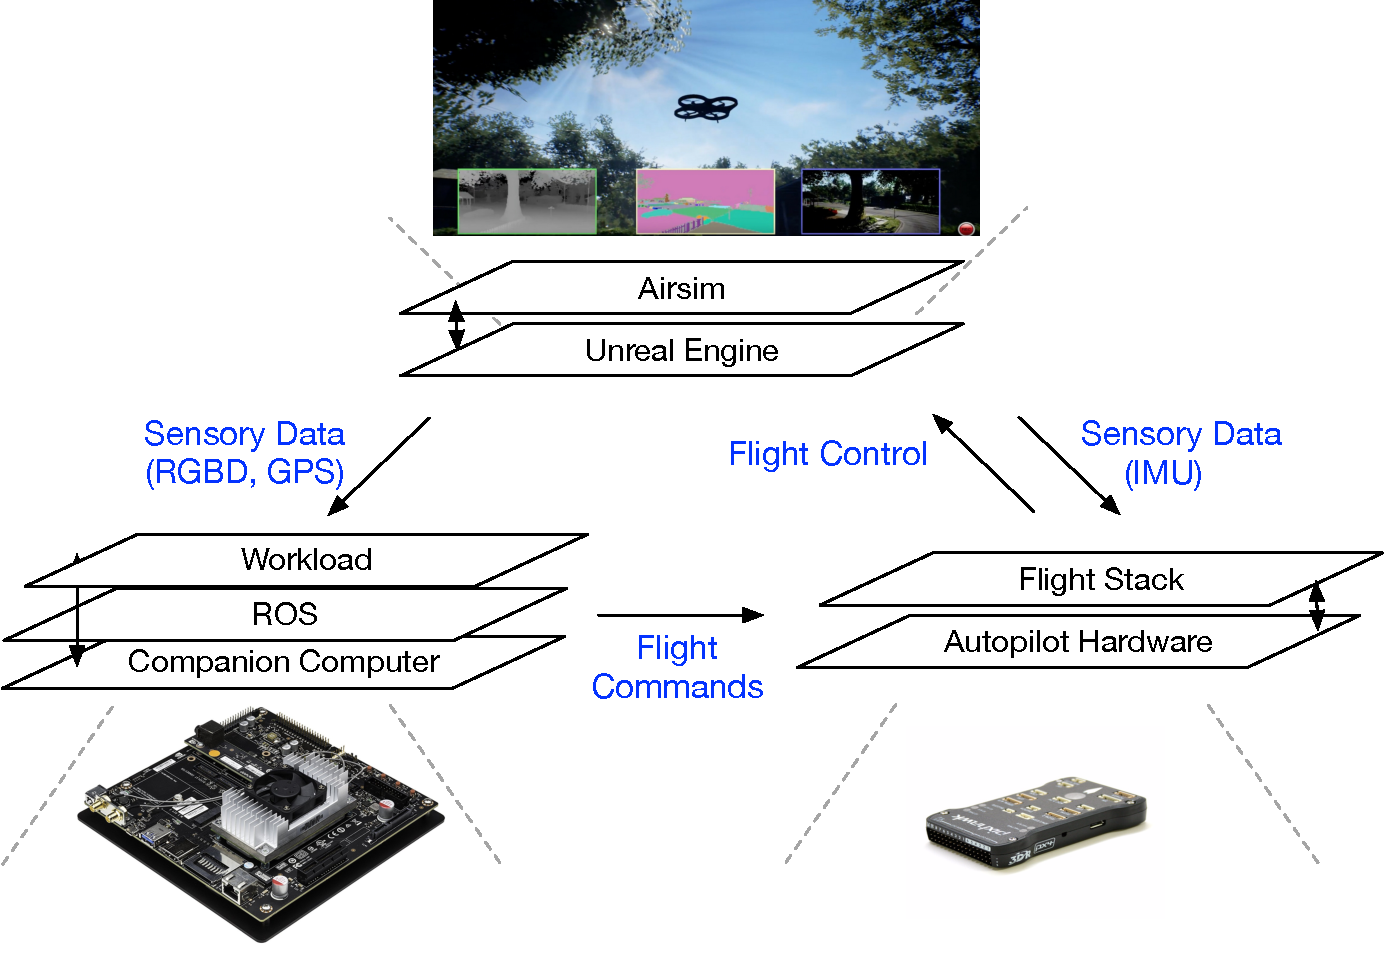
\includegraphics[trim= 10 10 10 10, clip, width=0.75\columnwidth]{figs/end-to-end-simulation}
\caption{Architectural overview of our closed-loop simulation. 
%\red{change airsim to UNREAL + Airsim: possibly annotate them with env and MAV (maybe even sensors/actuators)}}
}
\label{fig:end-to-end}
\end{figure}

\paragraph{Environments, Sensors and Actuators:} Environments, sensors and actuators are simulated with the help of a game engine called Unreal~\cite{GameEngi70:online}. With a physics engine at its heart, it ``provides the ability to perform accurate collision detection as well as simulate physical interactions between objects within the world''~\cite{PhysicsS8:online}. Unreal provides a rich set of environments such as mountains, jungles, urban setups, etc. to simulate.

To capture a MAV's dynamics and kinematics through its actuators' behavior and its sensory modules, we used AirSim, an open-source Unreal based plug-in from Microsoft~\cite{Airsim:online}. We limit our sensors and actuators to the ones realistically deployable by MAVs, such as \mbox{RGB-D} cameras and IMUs. Unreal and Airsim run on a powerful computer (host) capable of physical simulation and rendering. Our setup uses an Intel Core i7 CPU and a high-end NVIDIA GTX 1080 Ti GPU.  

\paragraph{Flight Controller:} AirSim supports various flight controllers that can be either hardware-in-the-loop or completely software-simulated. For our experiments, we chose the default software-simulated flight controller provided by AirSim. However, AirSim also supports other FCs, such as the Pixhawk~\cite{Pixhawk:online}, shown in black in \Fig{fig:end-to-end} which runs the PX4~\cite{PX4Archi7:online} software stack. AirSim supports any FC which can communicate using MAVLINK, a widely used micro aerial vehicle message marshaling library~\cite{mavlinkm68:online}. %MAVLINK is supported as the communication protocol by an extensive number of autopilot systems.
%\red{we should somehow here or later mention that we actually are using the airsim's simple FC instead of pixhawk}


\paragraph{Companion Computer:} We used an NVIDIA Jetson TX2~\cite{TX2}, a high-end embedded platform from Nvidia with 256 Pacal CUDA cores GPU and a Quad ARM CPU; however, the flexibility of our setup allows for swapping this embedded board with others such as x86 based Intel Joule~\cite{joule:online}. TX2 communicates with Airsim and also FC via Ethernet.

\paragraph{ROS:} Our setup uses the popular Robot Operating System (ROS) for various purposes such as low-level device control and inter-process communication~\cite{ROSorgPo80:online}.
Robotic applications typically consist of many concurrently-running processes that are known as ``nodes.'' For example one node might be responsible for navigation, another for localizing the agent and a third for object detection. ROS provides peer-to-peer communication between nodes, either through blocking ``service'' calls, or through non-blocking FIFOs (known as the Publisher/Subscriber paradigm). % A Master node registers all other nodes in a table allowing the communication to take place. 

\paragraph{Workloads:} Our workloads runs within the ROS runtime on TX2. They are extensively discussed in \Sec{sec:benchmarks}.

\paragraph{Putting It All Together:} To understand the flow of data, we walk the reader through a simple workload where the MAV is tasked to detect an object and fly toward it. The object (e.g. a person) and its environment (e.g. urban) are modeled in the Unreal Engine. As can be seen in \Fig{fig:end-to-end}, the MAV's sensors (e.g. accelerometer and \mbox{RGB-D} Camera), modeled in Airsim, feed their data to the flight controller (e.g. physics data to PX4) and the companion computer (e.g. visual and depth to TX2) using MAVLink protocol. The kernel (e.g. object detection), running within the ROS runtime environment on the companion computer, is continuously invoked until the object is detected. Once so, flight commands (e.g. move forward) are sent back to flight controller, where they get converted to a low level rotor instruction stream flying the MAV closer to the person. 

\subsection{Energy Simulation and Battery Model}
\label{sec:energy}

We extended the AirSim simulation environment with an energy and a battery model. Our energy model is a function of the velocity and acceleration of the MAV~\cite{energyaware}. The higher the velocity or acceleration, the higher the amount of energy consumption. Velocity and acceleration values are sampled continuously, their associated power calculated and integrated for capturing the total energy consumed by the agent.

\newcommand{\norm}[1]{\left\lVert#1\right\rVert}

We used a parametric power estimation model proposed in \cite{3DR-energy-model}. The formula for estimating power $P$ is described below:%
\begin{equation}
\begin{aligned}
P = \begin{bmatrix}
		\beta_{1} \\
		\beta_{2} \\
		\beta_{3}
	\end{bmatrix}^{T}
    \begin{bmatrix}
		\norm{\vec{v}_{xy}} \\
		\norm{\vec{a}_{xy}} \\
		\norm{\vec{v}_{xy}}\norm{\vec{a}_{xy}}
	\end{bmatrix}
    +
    \begin{bmatrix}
		\beta_{4} \\
		\beta_{5} \\
		\beta_{6}
	\end{bmatrix}^{T}
    \begin{bmatrix}
		\norm{\vec{v}_{z}} \\
		\norm{\vec{a}_{z}} \\
		\norm{\vec{v}_{z}}\norm{\vec{a}_{z}}
	\end{bmatrix}
    \\
    +
    \begin{bmatrix}
		\beta_{7} \\
		\beta_{8} \\
		\beta_{9}
	\end{bmatrix}^{T}
    \begin{bmatrix}
		m \\
		\vec{v}_{xy} \cdot \vec{w}_{xy} \\
		1
	\end{bmatrix}
\end{aligned}
\label{eqn:power}
\end{equation}

In the Equation~\ref{eqn:power}, $\beta_{1}$, ..., $\beta_{9}$ are constant coefficients determined based on the simulated drone. $\vec{v}_{xy}$ and $\vec{a}_{xy}$ are the horizontal speed and acceleration vectors whereas  $\vec{v}_{z}$ and $\vec{a}_{z}$ are the corresponding vertical values. $m$ is the mass and $\vec{w}_{xy}$  is the vector of wind movement. 

We have a battery model that implements a coulomb counter approach~\cite{coulomb-counter}. The simulator calculates how many coulombs (product of current and time) have passed  through the drone's battery over every cycle. This is done by calculating the power and the voltage associated with the battery. The real-time voltage is modeled as a function of the percentage of the remaining coulomb in the battery as described in ~\cite{battery-model}.

\subsection{Simulation Knobs and Extensions}
\label{sec:knobs}

With the help of Unreal and AirSim, our setup exposes a wide set of knobs. Such knobs enable the study of agents with different characteristics targeted for a range of workloads and conditions. For different environments, the Unreal market provides a set of maps free or ready for purchase. Furthermore, by using Unreal programming, we introduce new environmental knobs, such as (static) obstacle density, (dynamic) obstacle speed, and so on. In addition, Unreal and AirSim allow for the MAV and its sensors to be customized. For example, the cameras' resolution, their type, number and positions all can be tuned according to the workloads' need.   

Our simulation environment can be extended. For the compute on the edge, the TX2 can be replaced with other embedded systems or even micro-architectural simulators, such as gem5. Sensors and actuators can also be extended, and various noise models can be introduced allowing for reliability studies. 

\subsection{Simulation Fidelity and Limitations}
\label{sec:accuracy}

The fidelity of our end-to-end simulation platform is subject to different sources of error, as it is with any simulation setup. The major obstacle is the \textit{reality gap}---i.e., the difference between the simulated experience and the real world. This has always posed a challenge for robotic systems. The discrepancy results in difficulties where the system developed via simulation does not function identically in the real world. 

To address the reality gap, we iterate upon our simulation components and discuss their fidelity and limitations. Specifically, this involves (1) simulating the environment, (2) modeling the drone's sensors and flight mechanics, and last but not least (3) evaluating the compute subsystem itself.

First, the Unreal engine provides a high fidelity environment. By providing a rich toolset for lighting, shading, and rendering, photo-realistic virtual worlds can be created. In prior work~\cite{unrealcv}, authors examine photorealism by running a Faster-RCNN model trained on PASCAL in an Unreal generated map. The authors show that object detection precision can vary between 1 and 0.1 depending on the elevation and the angle of the camera. Also, since Unreal is open-sourced, we pro grammatically emulate a range of real-world scenarios. For example, we can set the number of static obstacles and vary the speed of the dynamic ones to fit the use case.   

Second, AirSim provides high fidelity models for the MAV, its sensors and actuators. Embedding these models into the environment in a real-time fashion, it deploys a physics engine running with 1000~\si{\hertz}.  As the authors discuss in~\cite{Airsim_paper}, the high precision associated with the sensors, actuators and their MAV model, allows them to simulate a Flamewheel quadrotor frame equipped with a Pixhawk~v2 with little error. 

Flying a square-shaped trajectory with sides of length 5~\si{\meter} and a circle with a radius of 10~\si{\meter},  AirSim achieves  0.65~\si{\meter} and 1.47~\si{\meter} error, respectively. Although they achieve high precision, the sensor models, such as the ``camera lens models,'' ``degradation of GPS signal due to obstacles,'' ``oddities in camera,'' etc. can benefit from further improvements. %\red{somewhere we should mention that we extended airsim to use DJI Matrice}

Third, as for the compute subsystem itself, our hardware has high fidelity since we use off-the-shelf embedded platforms for both the companion computer and the flight controller. As for the software, it is crucial to note ROS is widely used and adopted as the \textit{de facto} OS in the robotics research community.

%The details of the simulation environment components' precisions resulting in the aforementioned error is further discussed in~\cite{Airsim_paper}.

%\subsection{Simulation Limitations}
%\label{sec:limits}

%\paragraph{Network Bottleneck:} As was previously mentioned, our companion computer and Airsim are connected through Ethernet. Hence, transferring multiple high resolution images can be throttled by the cable's bandwidth. 

\begin{comment}
Using such data, one can define  various metrics for the applications of interest. For example, using time to delivery over the amount of energy spent, one can define an efficiency metric for a package delivery application. Metrics are extensively discussed in the section \ref{MAVBench characterization}.
\end{comment}
\begin{comment}
\begin{figure*}[h]
\centering
\includegraphics[width=.3\linewidth]{figs/blank}
\includegraphics[width=.3\linewidth]{figs/blank}
\includegraphics[width=.3\linewidth]{figs/blank}
\caption{Show a picture of what AirSim is doing and what the "MAV" is seeing.}
\label{fig:end-to-end}
\end{figure*}
\end{comment}

\begin{comment}

\subsection{Workloads} \label{ssec:benchmarks}

\red{here we explain the workloads we are using for our study, going into the details of each and perhaps even explaining what computational kernels they are exercising. the table of the workloads should discuss the internal details of th apps.}

Our workloads are organized into a full benchmark suite that tests a MAV's ability to perform the tasks required for popular MAV applications today as well as MAV applications that are expected to become significant in the near-future.

Our benchmark suite is divided into two categories: a set of micro-benchmarks that test narrow MAV capabilities and a set of macro-benchmarks that test full MAV applications.

\subsubsection{Micro-benchmarks} \label{sssec:micro}

Our micro-benchmarks test a MAV's ability to execute tasks that would be part of a full MAV application, such as computational kernels or simple flight maneuvers. The micro-benchmarks themselves, however, do not represent complete MAV applications.

The micro-benchmarks primarily stress a MAV's computer vision, SLAM, and pathfinding capabilities. A few of the micro-benchmarks do not test any computational capabilities at all, but are instead meant to characterize a MAV's power consumption during flight. Our micro-benchmarks are listed in full in Table~\ref{tab:micro}.




\subsubsection{Macro-benchmarks} \label{sssec:macro}

Our macro-benchmarks, described in Table~\ref{tab:macro} are complete MAV applications that characterize a MAV's performance and power consumption when performing typical MAV applications. The macro-benchmarks are made up the smaller kernels that are tested by the micro-benchmarks described in Sec.~\ref{sssec:micro}.

\begin{table*}[h!]
\begin{tabular*}{\textwidth}{l@{\extracolsep{\fill}}lllll}
\hline
Benchmark & Use Case & Kernel(s)\\\hline
\texttt{outdoor\_track} & Target tracking (sports photography) & Computer vision; object detection \\
\texttt{indoor\_track} & Target tracking (indoors) & Computer vision; object detection \\
\texttt{deliver} & Package delivery & Pathfinding; SLAM; computer vision \\
\texttt{search} & Search and rescue & Computer vision; object detection; SLAM \\
\texttt{survey} & Land surveying & \fxnote{nothing really} \\
\texttt{map} & Mapping a building & Computer vision; image stitching \\
\texttt{data\_coverage} & Wireless data coverage & \fxnote{?} \\
\texttt{driving} & Autonomous navigation & Machine learning \\
\texttt{take\_picture} & Go to target address, take picture, and return & Path planning \\
\hline
\end{tabular*}
\caption{Macro-benchmarks.}
\label{tab:macro}
\end{table*}

\subsection{Platforms} \label{ssec:MAVs}

\red{here we provide the specific platforms we have evaluated, and for the most part these will be the architectural capabilities of the compute boards that corresponds to our different MAV platforms.}

% Description of our MAV platforms, including a table giving details on each one's weight, flight controller, etc.

We characterize a variety of MAV processors and MAV platforms, both physical and simulated, using our benchmark suite. Our power characterizations are based primarily upon our physical MAVs, described in Table~\ref{tab:MAV-platforms}. Our performance characterizations are primarily based upon workloads run on a simulated MAV known as Microsoft AirSim~\cite{}, rather than on physical MAV platforms.

\paragraph{Processors} We run our computational workloads on a variety of embedded processors, described in Table~\ref{}, that are targeted towards MAVs and robotics applications. These range from state-of-the-art embedded systems with powerful CPUs and hundreds of GPU cores all the way to smartphone-level processors such as the i.MX6 with much lower performance capabilities.

\begin{table*}[t!]
\centering
\caption{Companion computer characteristics.}
\label{tab:cc-platforms}
\begin{tabular}{ l | c c c c c }
 \hline \noalign{\vskip 0.5mm}
 & Intel Aero & Jetson TX1 & Intel Joule & i.MX6 Solo & ODroid  \\
 \hline \noalign{\vskip 0.5mm}
 % SOC    	& Intel Atom 7-Z8750 & \\
 CPU    	& Intel Atom 7-Z8750 & ARM Cortex-A57 & Intel Atom T5700 & ARM Cortex A9 \\
\ \ Frequency	& 1.60 GHz & \fxnote{Unpublished} & 1.7 GHz & 1 GHz \\
\ \ L1 \$ (I/D) & 226 KiB & 80 KB & \fxnote{Unknown}  & 64 KB \\
\ \ L2 \$ (I/D) & 2 MiB & 2 MB  & 2x2 MB & 512 KB \\
\ \ Cores 	& 4 & 4 & 4 & 1 \\
 GPU    	& Intel HD Graphics 405 & 256-core Maxwell GPU & Intel HD Graphics & Two integrated 3D and 2D GPUs\\
 RAM    	& 4 GB LPDDR3 & 4 GB LPDDR4 & 4 GB LPDDR4 & 512 MB \\
 OS     	& Yocto 2.1 (Linux 4.4.3) & Ubuntu 16.04 & Ubuntu 16.04 & 3DR Poky (based on Yocto) \\
 \hline
\end{tabular}
\end{table*}

\paragraph{Physical MAVs} We characterized the power consumption of MAVs ranging from X to Y lbs in weight. We investigated MAVs of different weights because a MAV's weight strongly affects its power consumption and is also correlated to its maximum payload which determines the weight of the components that can be placed upon it. 

% \paragraph{Microsoft AirSim} A simulated MAV with realistic video data. The setup is illustrated in Fig.~\ref{fig:end-to-end}.

\paragraph{Microsoft AirSim} AirSim is an HIL simulator of a micro-aerial vehicle that was developed to allow machine learning applications to easily and safely generate training data for their MAVs. AirSim runs on the Unreal engine and is thus capable of generating realistic video data for our MAV applications. Thus, AirSim allow us to develop realistic environments for our macro-benchmarks so that our characterizations can be easily run on MAV processors in a safe and repeatable fashion. The interfacing between our workloads, MAV processors, and AirSim itself in illustrated in Fig.~\ref{fig:end-to-end}.

\end{comment}
\section{Benchmark Suite} 
\label{sec:mavbench}

\begin{figure*}[t]
\centering
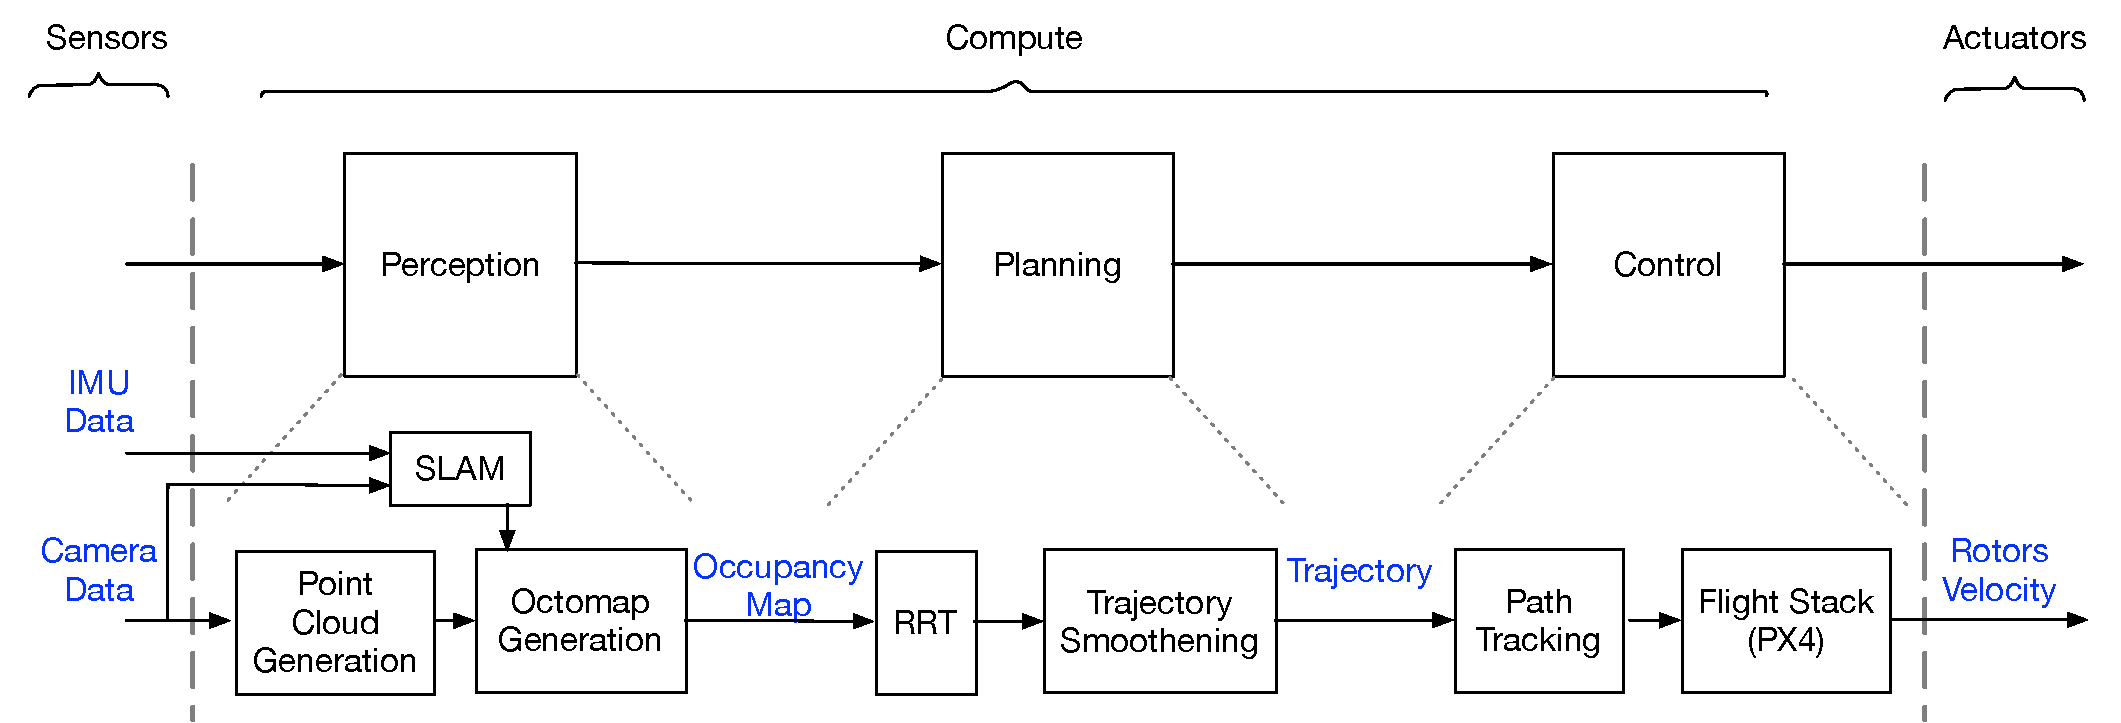
\includegraphics[height=1.65in, keepaspectratio]{figs/software_pipeline}
\caption{High-level application pipeline for a typical MAV application. The upper row presents a universal pipeline that all our MAVBench applications follow, which involves \emph{perception}, \emph{planning} and \emph{control}. The lower row presents how a specific workload in MAVBench (e.g. package delivery) maps to the universal high-level application pipeline.}
\label{fig:software_pipeline}
\end{figure*}


To quantify the power and performance demands of typical MAV applications, we created a set of workloads that we compiled into a benchmark suite. Our benchmarks run on top of our closed-loop simulation environment. The suite aims to cover a wide range of representative applications. Each workload is an \textit{end-to-end} application that allows us to study the kernels' impact on the whole application as well as to investigate the interactions and dependencies between kernel. 

By providing holistic end-to-end applications instead of only focusing on individual kernels, MAVBench allows for the examination of kernels' impacts and their optimization at the application level. This is a lesson learned from Amdahl's law, which recognizes that the true impact of a component's improvement needs to be evaluated globally rather than locally.

In \Sec{sec:sw_pipeline}, we present a high level software pipeline associated (though not exclusive) to our workloads. In \Sec{sec:benchmarks}, we present functional summaries of the workloads in MAVBench, their use cases, and mappings from each workload to the high level software pipeline. In \Sec{sec:kernels}, we describe in details of the prominent computational kernels that are incorporated into our workloads, and finally in \Sec{sec:QoF} we provide a short discussion regarding the Quality-of-Flight (QoF) metrics to evaluate MAV applications.

The MAVBench workloads have different computational kernels, as shown in Table~\ref{kernel_makeup}. MAVBench aims at being comprehensive by (1) selecting applications that target different robotic domains (robotics in hazardous areas, construction, etc.) and (2) choosing kernels (e.g. point cloud, RRT) common across a range of applications, not limited to our benchmark-suite. The computational kernels (OctoMaps, RTT, etc.) that we use in the benchmarks are the building blocks of many robotics applications and hence they are platform agnostic. 

% Our insights carry over to rotorcraft UAVs and AUVs (Autonomous underwater vehicles), since in both cases constant power is required to maintain the position. Furthermore, ground mobile robots under high energy constraints can also exploit principles presented.


% Application architecture section
% Add low-level details like which kernels we use
% Mention that we have flexibility
% Add small details like SLAM-backtracking, Octomap, ROS
% Add new paragraphs after every benchmark
% Some analysis of benchmarks (length of runtime, number of ROS nodes)
% Literature survey (PARSEC, BioBench, WHISPER)
% Add annotated graphics to system architecture showing sensors
% Draw an end-to-end diagram or a table
% Talk about core kernels to foreshadow future characterization


\subsection{Application Dataflow} \label{sec:sw_pipeline}

\begin{figure*}[t]
	\centering
	\begin{subfigure}[t]{1.385in}
		\centering
		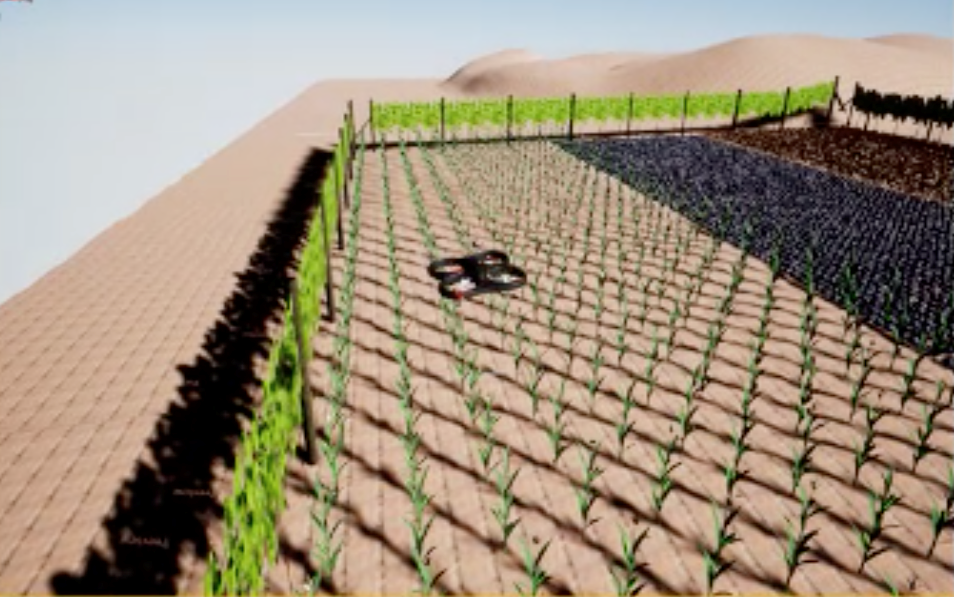
\includegraphics[width=\textwidth, height=1in]{figs/benchmarks/scanning}
		\caption{Scanning.}\label{fig:benchmarks:scanning}
	\end{subfigure}
	\hfill
	\begin{subfigure}[t]{1.385in}
		\centering
		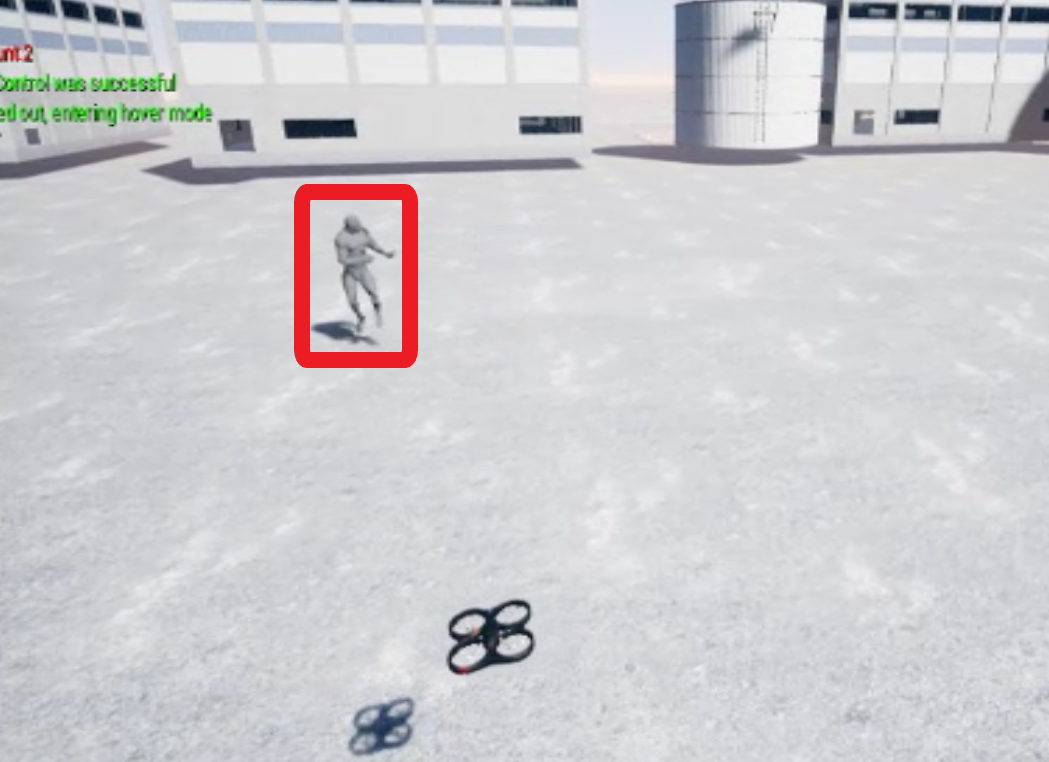
\includegraphics[width=\textwidth, height=1in]{figs/benchmarks/aerial-photo}
		\caption{Aerial Photography.}\label{fig:benchmarks:aerial-photo}
	\end{subfigure}
	\hfill
    \begin{subfigure}[t]{1.385in}
		\centering
		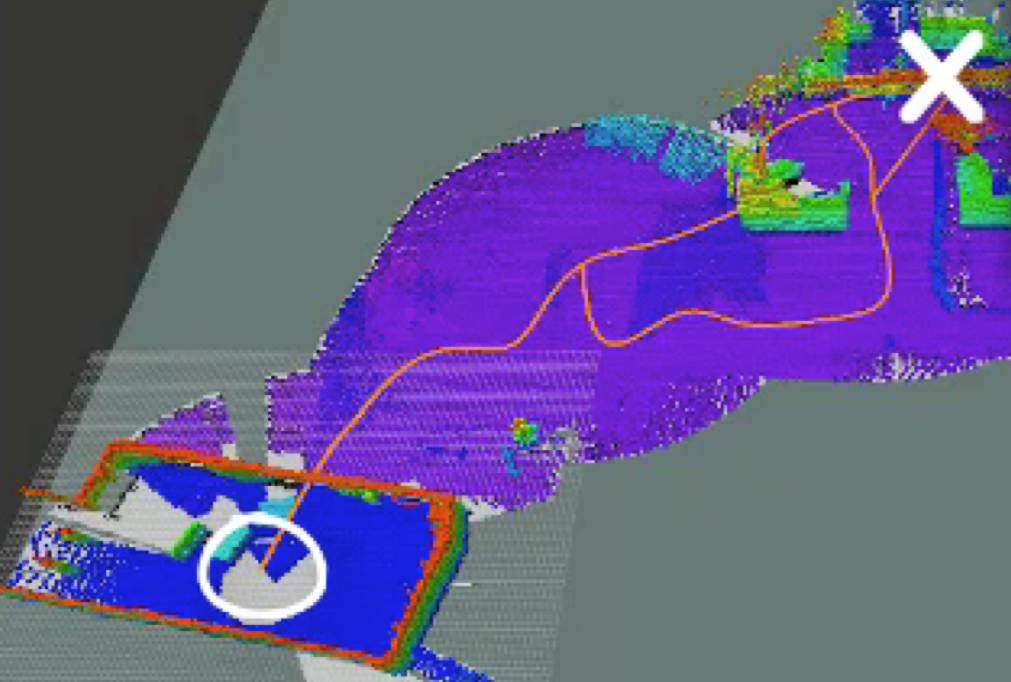
\includegraphics[width=\textwidth, height=1in]{figs/benchmarks/package-delivery}
		\caption{Package Delivery.}\label{fig:benchmarks:package-delivery}
	\end{subfigure}
	\hfill
    \begin{subfigure}[t]{1.385in}
		\centering
		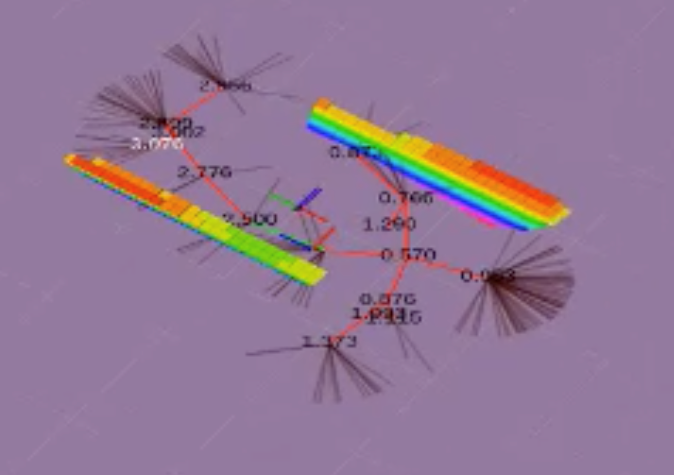
\includegraphics[width=\textwidth, height=1in]{figs/benchmarks/3d-mapping}
		\caption{3D Mapping.}\label{fig:benchmarks:3D-mapping}
	\end{subfigure}
	\hfill
    \begin{subfigure}[t]{1.385in}
		\centering
		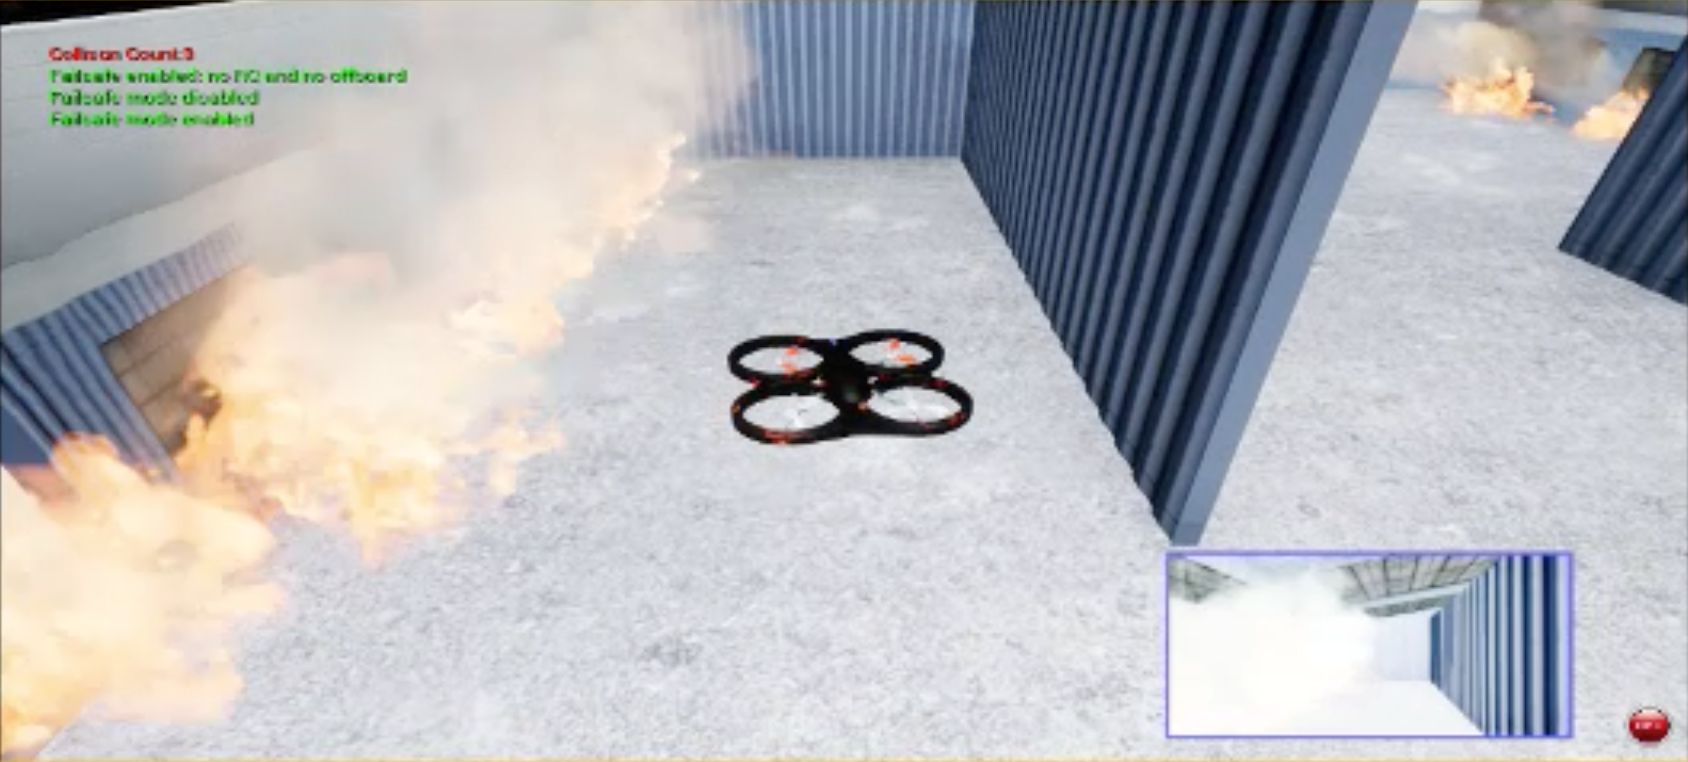
\includegraphics[width=\textwidth, height=1in]{figs/benchmarks/search-and-rescue}
        \caption{Search and Rescue.}\label{fig:benchmarks:search-and-rescue}
	\end{subfigure}
    \vspace{-5pt}
    \caption{MAVBench workloads. Each workload is an end-to-end application targeting both industry and research use cases. All figures are screenshots of a MAV executing a workload within its simulated environment. Fig.~\ref{fig:benchmarks:package-delivery} shows a MAV planning a trajectory to deliver a package. Fig.~\ref{fig:benchmarks:3D-mapping} shows a MAV sampling its environment in search of unexplored areas to map.}
    \label{fig:bench_screenshot}
\end{figure*}

\begin{figure}[t!]
	\centering
	\begin{subfigure}[t]{\columnwidth}
		\centering
        \vspace{-5pt}
		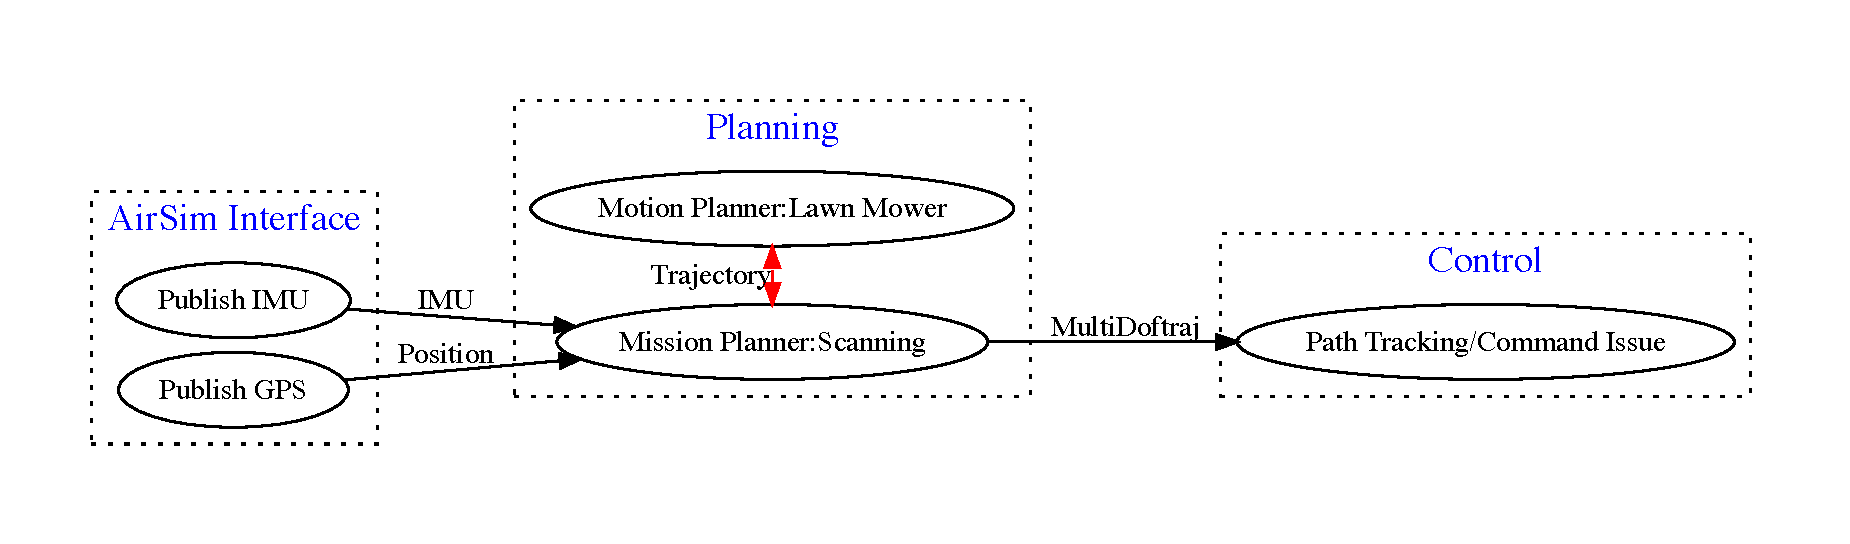
\includegraphics[width=\columnwidth]{figs/data_flow/scanning}
        \vspace{-20pt}
\caption{Scanning.}\label{fig:benchmarks:data-flow:scanning}
	\end{subfigure}
    %\vspace{-10pt}
    \begin{subfigure}[t]{\columnwidth}
		\centering
		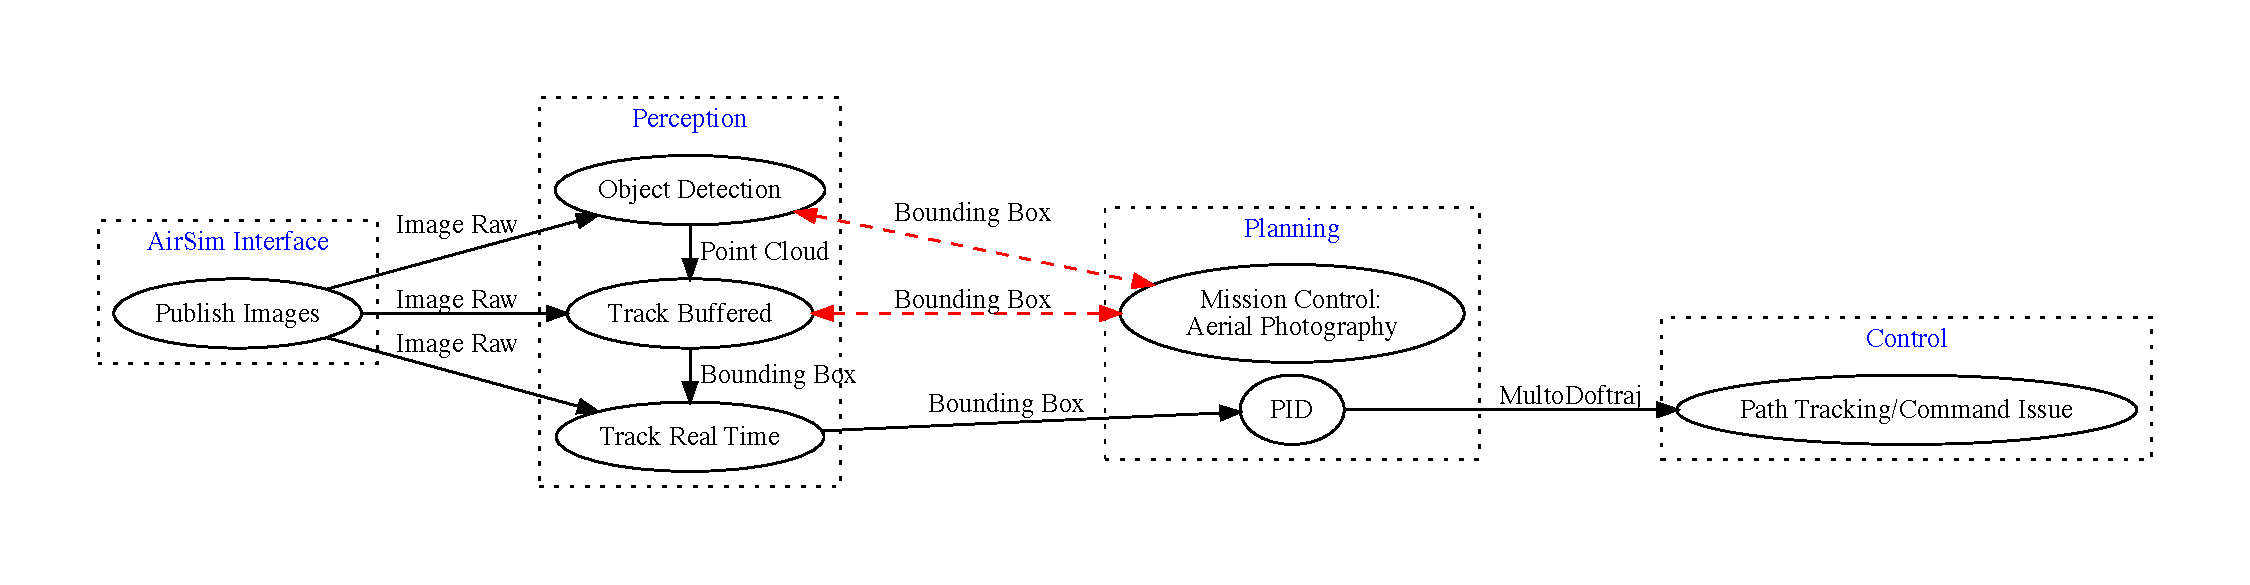
\includegraphics[width=\columnwidth]{figs/data_flow/aerial_photography}
        \vspace{-20pt}
		\caption{Aerial Photography.}\label{fig:benchmarks:data-flow:aerial_photography}
	\end{subfigure}
    %\vspace{-10pt}
	\begin{subfigure}[t]{\columnwidth}
		\centering
		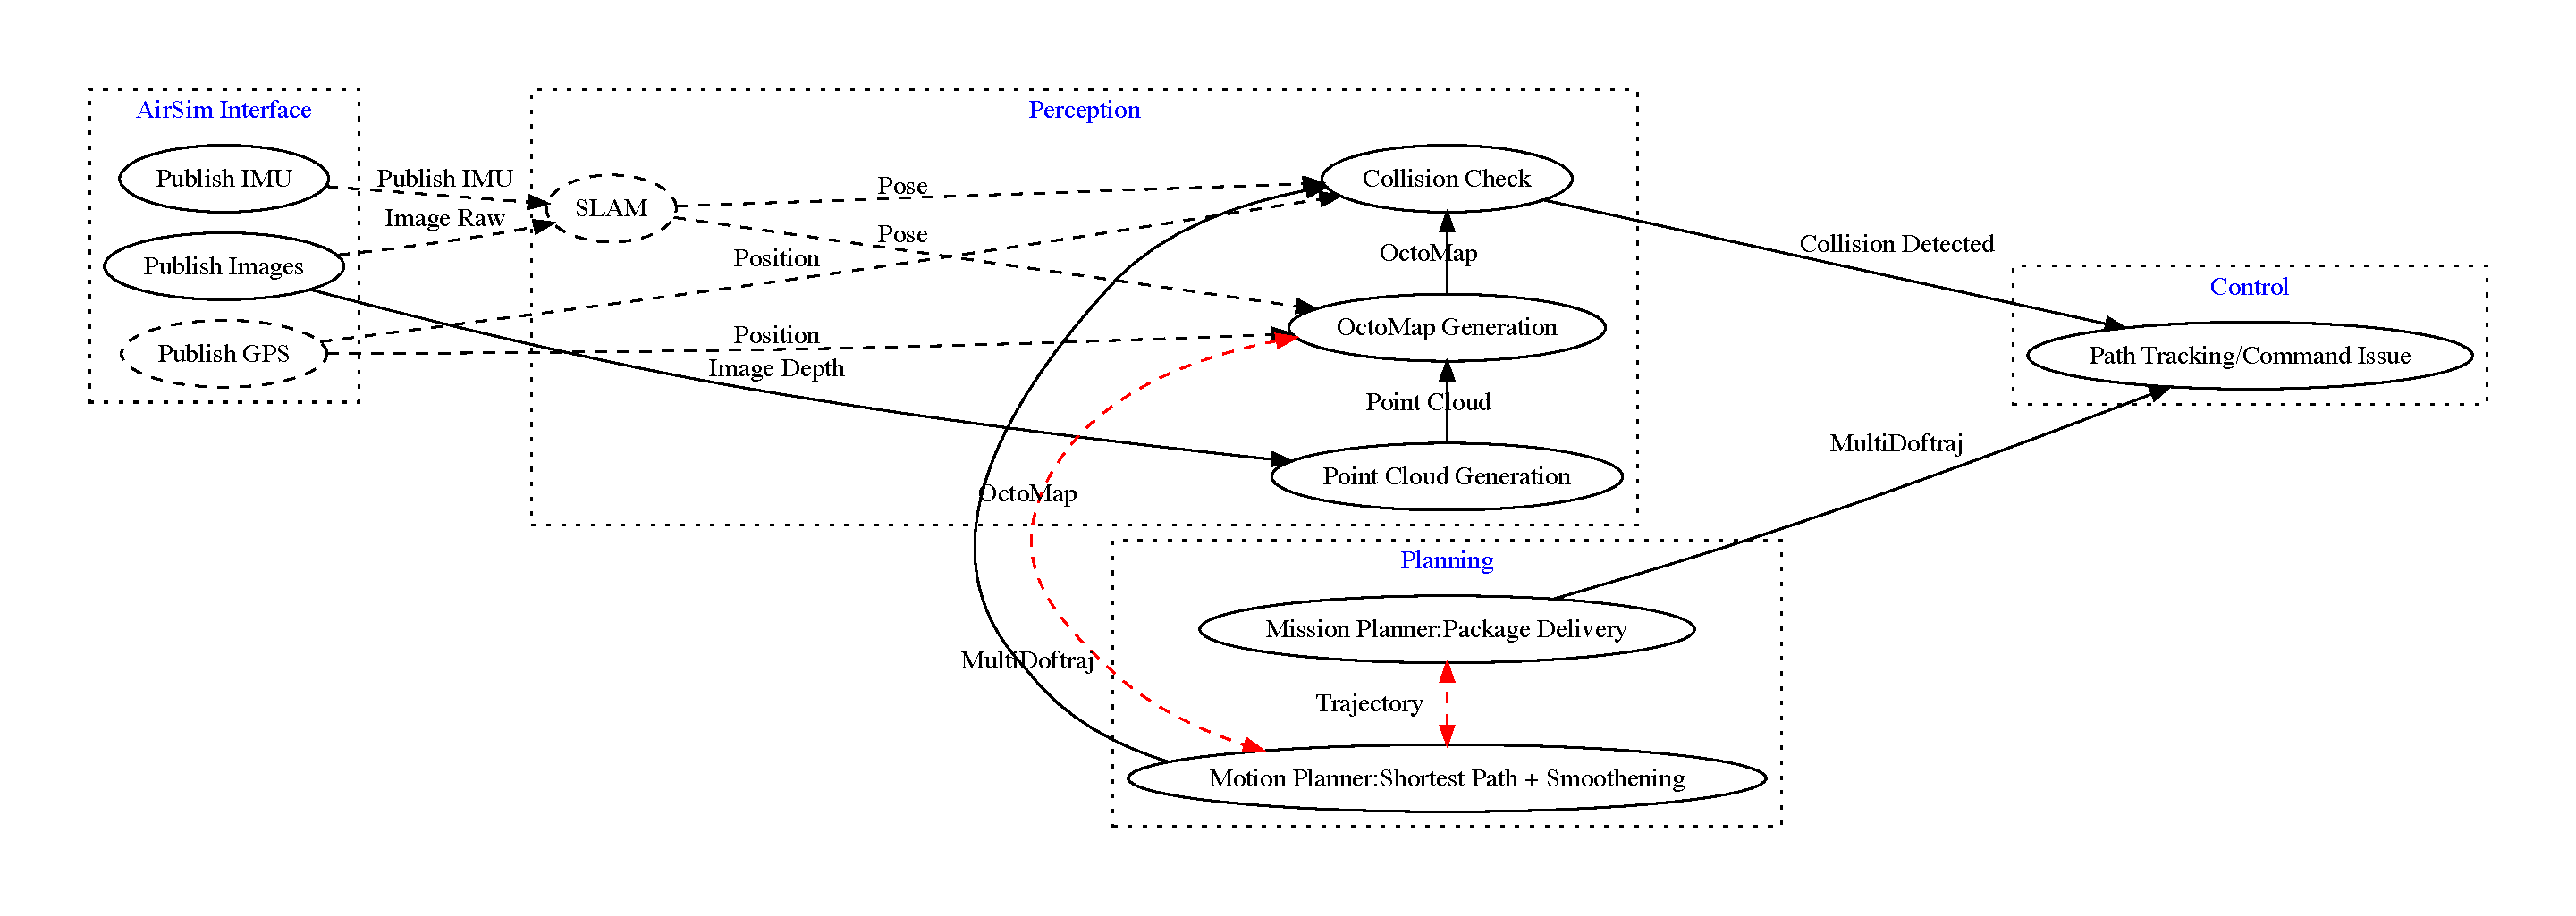
\includegraphics[width=\columnwidth] {figs/data_flow/package_delivery}
        \vspace{-20pt}
		\caption{Package Delivery.}\label{fig:benchmarks:data-flow:package_deilvery}
	\end{subfigure}
    %\vspace{-10pt}
    \begin{subfigure}[t]{\columnwidth}
		\centering
		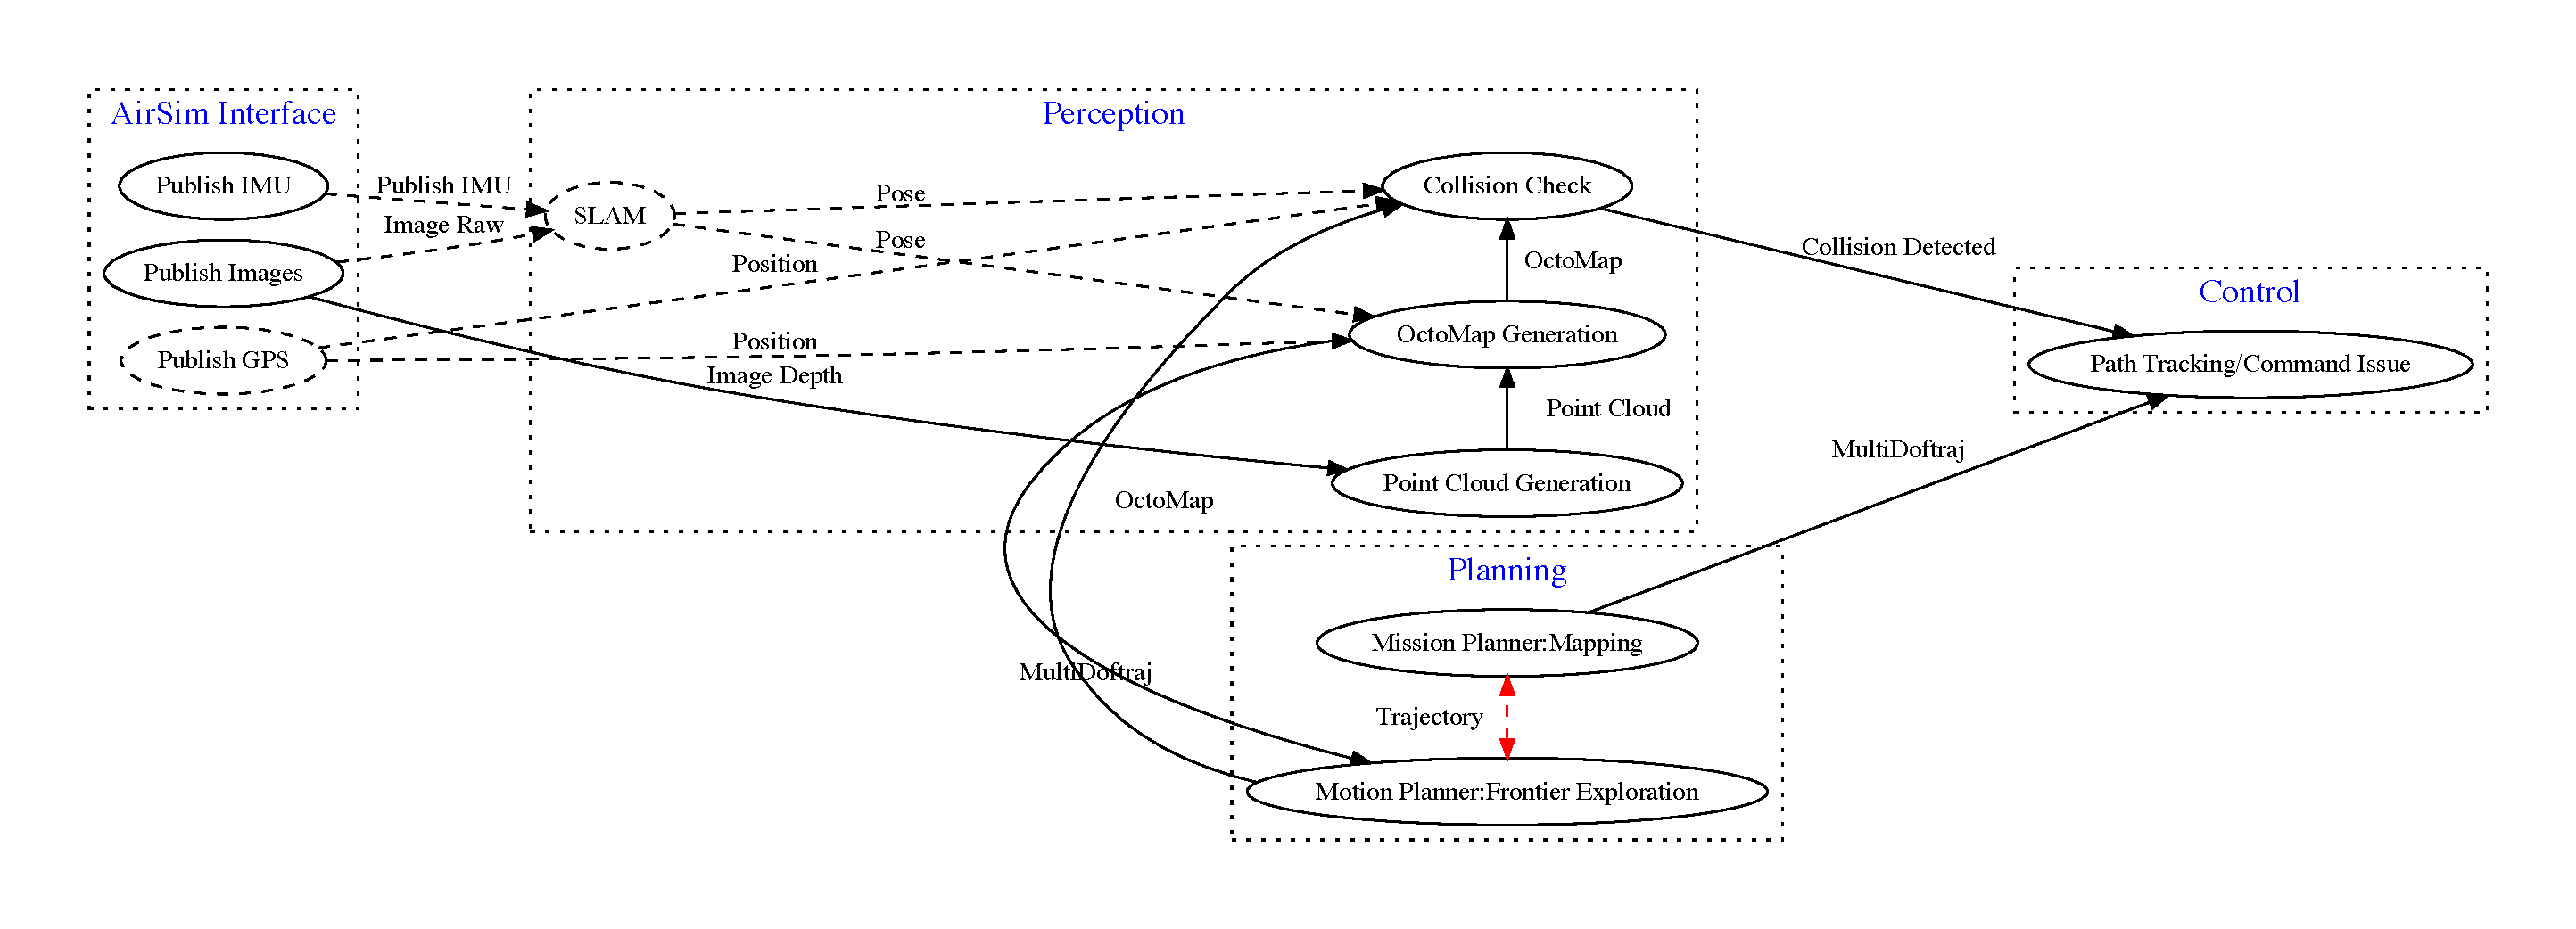
\includegraphics[width=\columnwidth]{figs/data_flow/mapping}
        \vspace{-20pt}
		\caption{3D Mapping.}\label{fig:benchmarks:data-flow:mapping}
	\end{subfigure}
    %\vspace{-10pt}
    \begin{subfigure}[t]{\columnwidth}
		\centering
		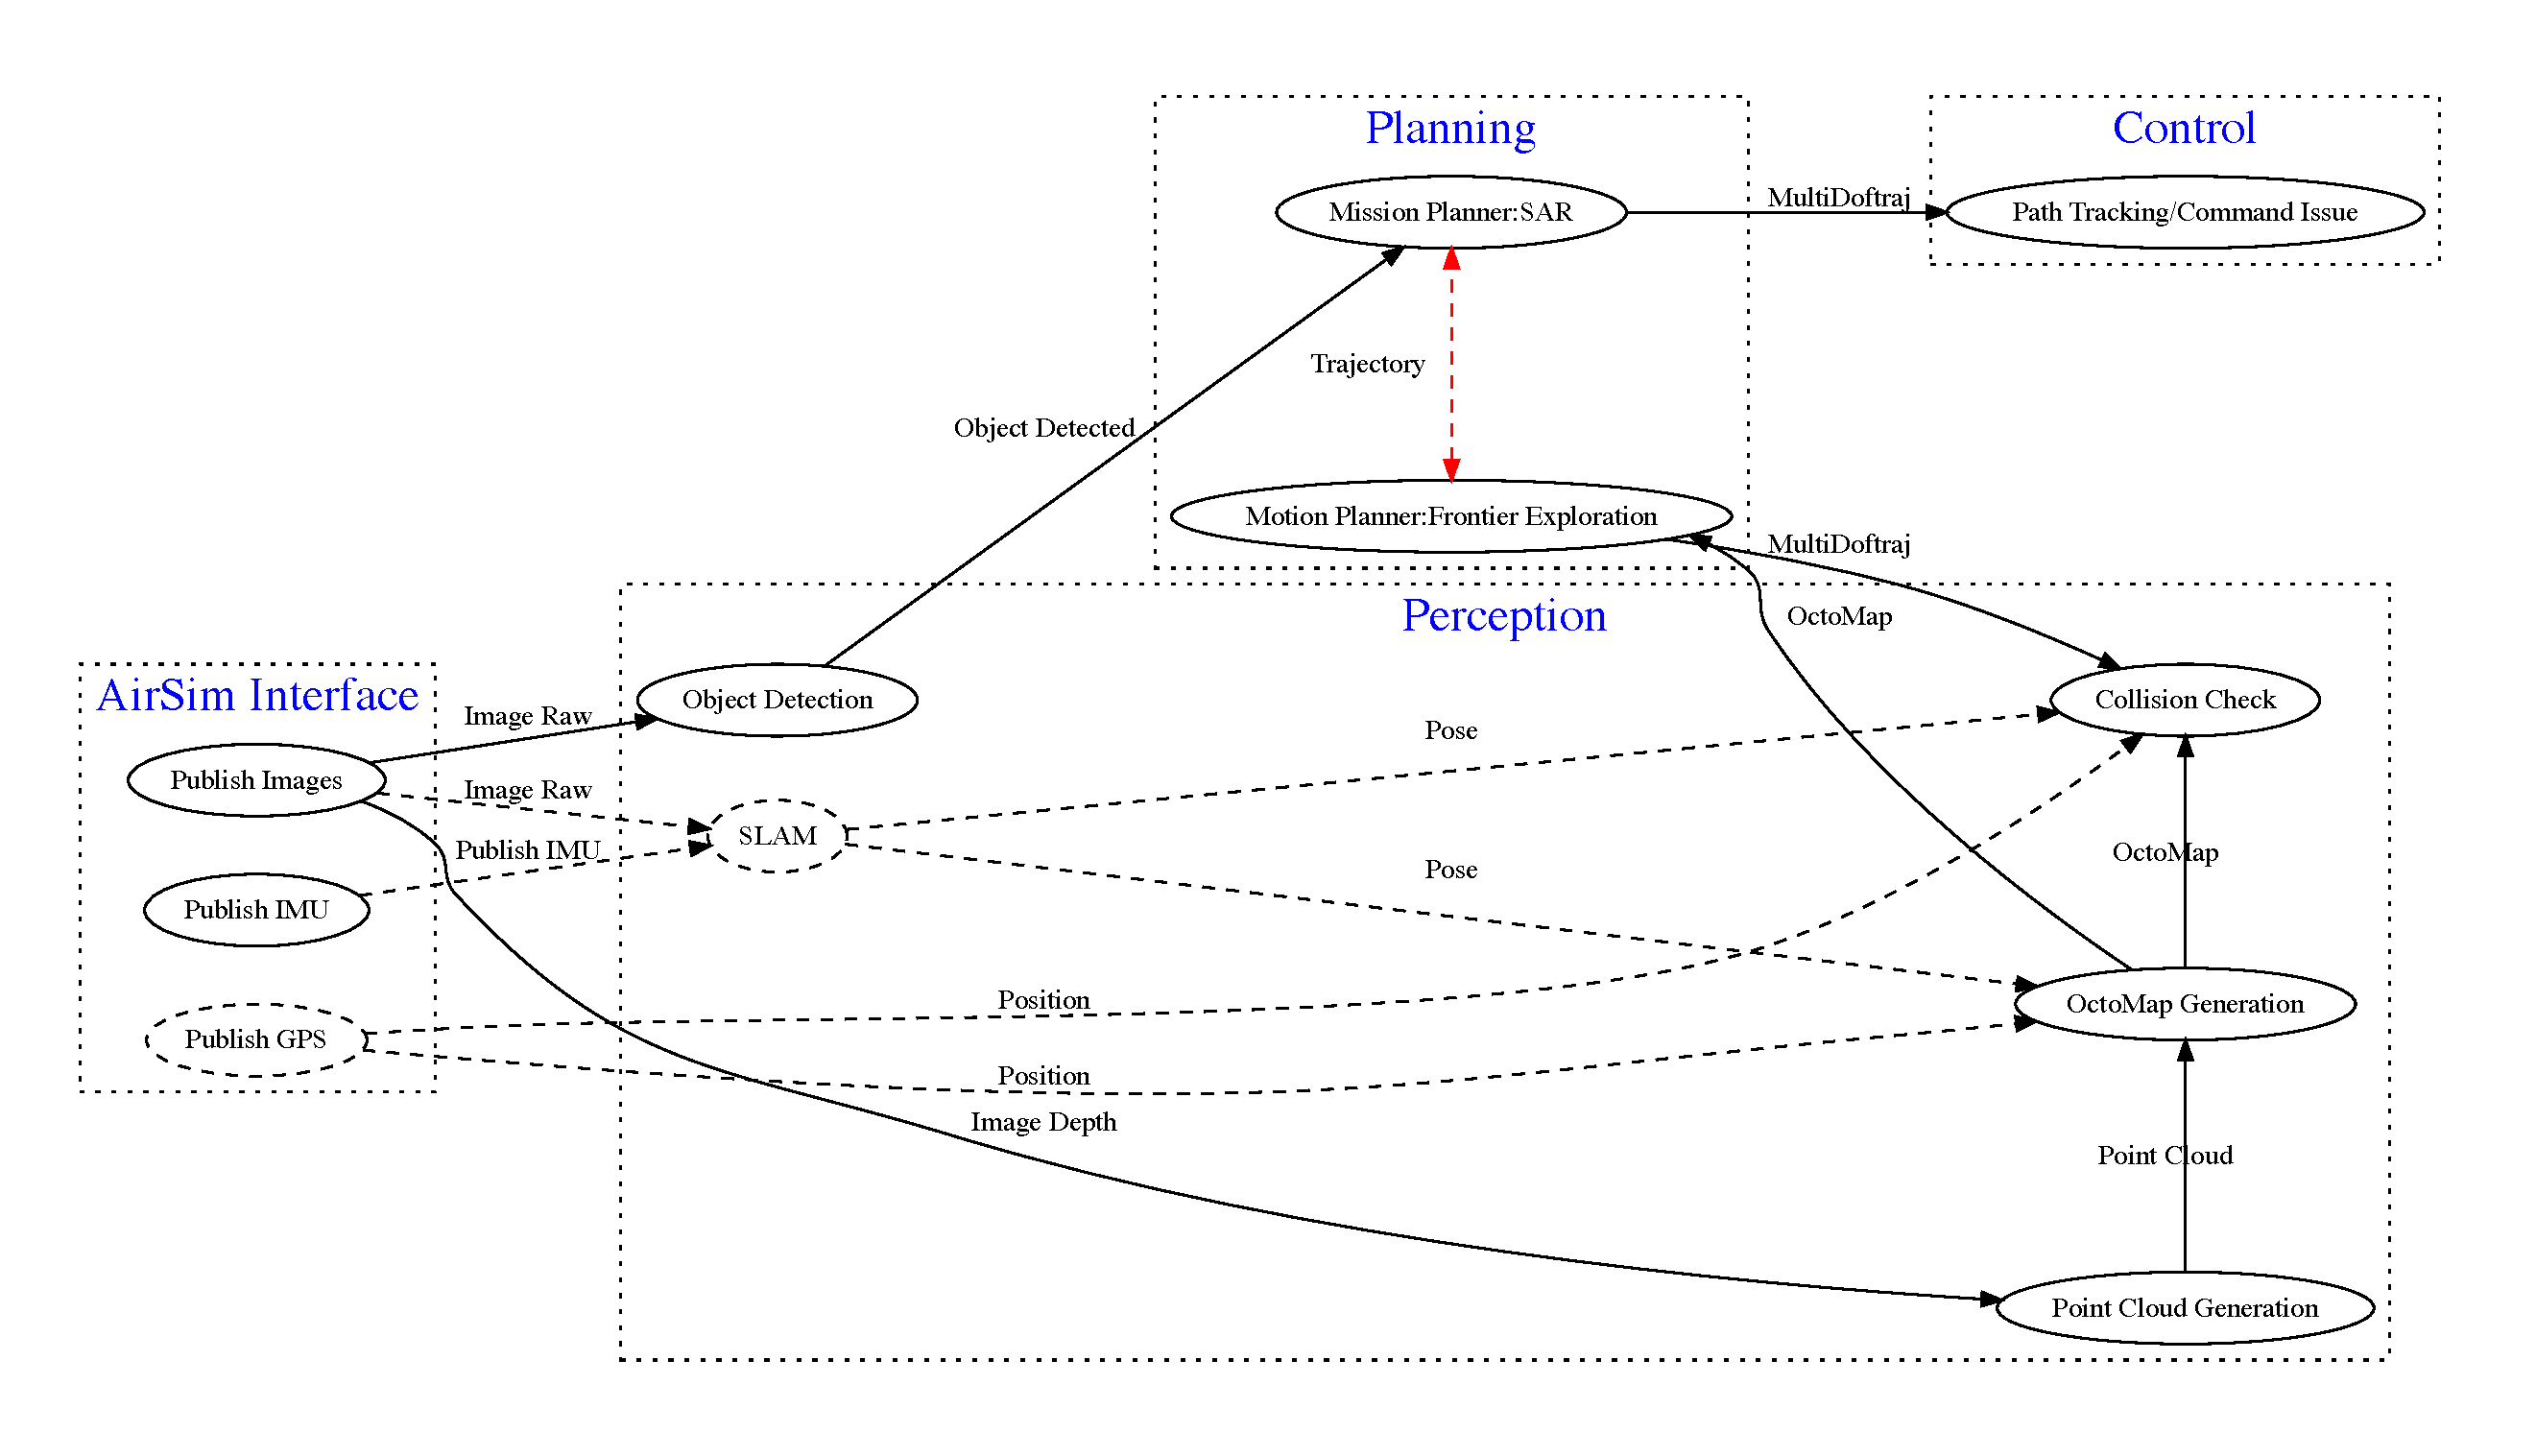
\includegraphics[width=\columnwidth]{figs/data_flow/sar}
        %\vspace{-20pt}
		\caption{Search and Rescue.}\label{fig:benchmarks:data-flow:sar}
	\end{subfigure}
    \caption{Application dataflows. Nodes are denoted with a circle and communication between the nodes is captured with an arrow. If the communication paradigm between the nodes is of a subscriber/publisher kind, the arrows are filled and black, whereas in the case of the client/server paradigm, they are dotted and red. Nodes with a subscriber/publisher communication paradigm or without any at all run in parallel. Dotted lines denote various localization techniques.}
    \label{fig:benchmarks_data_flow}
\end{figure}

There are three fundamental processing stages in each application: \emph{Perception}, \emph{Planning} and \emph{Control}. In the perception stage, the sensory data is processed to extract relevant states from the environment and the drone. This information is fed into the next two stages (i.e., planning and control). Planning ``plans'' flight motions and forwards them to the actuators in the control subsystem. \Fig{fig:software_pipeline} summarizes this high-level software pipeline, which each of our workloads embody.

\textbf{Perception:}
It is defined as ``the task-oriented interpretation of sensor data''~\cite{Handbook_robotic}. Inputs to this stage, such as sensory data from cameras or depth sensors, are fused to develop an elaborate model in order to extract the MAV's and its environment's relevant states (e.g. the positions of obstacles around the MAV). This stage may include tasks such as Simultaneous Localization and Mapping (SLAM) that enables the MAV to infer its position in the absence of GPS data.

\textbf{Planning:}
 Planning generally involves generating a \textit{collision-free} path to a target using the output of the perception (e.g. a occupancy map of obstacles in the environment). In short, this step involves first generating a set of possible paths to the target, such as by using the probabilistic roadmap (PRM) algorithm, and then choosing an optimal one among them using a path-planning algorithm, such as A*.

\textbf{Control:}
This stage is about following a desired path, which is absorbed from the previous stage, while providing a set of guarantees such as feasibility, stability and robustness~\cite{tech_problem}. In this stage, the MAV's kinematics and  dynamics are considered, such as by smoothening paths to avoid high-acceleration turns, and then, finally, the flight commands are generated (e.g. by flight controllers such as the PX4) while ensuring the aforementioned guarantees are still respected.

\subsection{Benchmarks} \label{sec:benchmarks}
The MAVBench benchmark suite consists of five workloads, each equipped with the flexibility to configure its computational kernel composition (described later in \Sec{sec:kernels}).
%\red{Although only containing 5 end-to-end applications, MAVBench has 13 computationally intensive kernels (table blah). MAVBench aims at being comprehensive by 1.selecting applications carefully such that each targets a different robotic's domain (e.g. Robotics in Hazardous Applications, Construction, ...) 2. selecting kernels (e.g. point cloud, RRT, ...) common across a wide range of applications and not limited to our benchmark-suite.  
%We also believe that by providing end-to-end applications instead individual kernels (cite paper blah and blah), MAVBench allows for examination of  kernels' impacts and their optimization at the application level. This is a lesson learned from  Amdahl's law, which recognizes that the true impact of a component's improvement needs to be evaluated globally rather than locally.} 
The following section sheds light on their functional summary. In addition, the inner workings of these workloads are explained in terms of the three-stage high-level application pipeline. \Fig{fig:bench_screenshot} presents screenshots of these different workloads. The application dataflows are shown in \Fig{fig:benchmarks_data_flow}.

\textbf{Scanning:} In this simple though popular use case, a MAV scans an area specified by its width and length while collecting sensory information about conditions on the ground. It is a common agricultural use case. For example, a MAV may fly above a farm to monitor the health of the crops below. To do so, the MAV first uses GPS sensors to determine its location (Perception). Then, it plans an energy efficient ``lawnmower path'' over the desired coverage area, starting from its initial position (Planning). Finally, it closely follows the planned path (Control). While in-flight, the MAV can collect data on ground conditions using on-board sensors, such as cameras or LIDAR. 


%This workloads QOS can be defined as both the mission time and the energy consumption of the mission.

\textbf{Aerial Photography:} Drone aerial photography is an increasingly popular use of MAVs for entertainment, as well as businesses. In this workload, we design the MAV to follow a moving target with the help of computer vision algorithms. The MAV uses a combination of object detection and tracking algorithms to identify its relative distance from a target (Perception). Using a PID controller, it then plans motions to keep the target near the center of the MAV's camera frame (Planning), before executing the planned motions (Control).
%The workload's QOS can be defined as average distance of the target from the center of camera frame. 

\textbf{Package Delivery:} In this workload, a MAV navigates through an obstacle-filled environment to reach some arbitrary destination, deliver a package and come back to its origin. Using a variety of sensors such as RGBD cameras or GPS, the MAV creates an occupancy map of its surroundings (Perception). Given this map and its desired destination coordinate, it plans an efficient collision-free path. To accommodate for the feasibility of maneuvering, the path is further smoothened to avoid high-acceleration movements (Planning), before finally being followed by the MAV (Control). While flying, the MAV continuously updates its internal map of its surroundings to check for new obstacles, and re-plans its path if any such obstacles obstruct its planned trajectory.
%QOS for this workload can consider both energy and mission time. 
%Additionally, the MAV is responsible for accurately localizing itself at all times, to determine its distance from its destination. If the MAV is outdoors, then this localization can easily be done using GPS, but in a GPS-denied environment, the MAV must instead rely upon SLAM algorithms such as ORB-SLAM2, which uses stereo or RGBD cameras, or VINS-MONO~\cite{vins-mono}, which uses a monocular camera paired with IMU data.

\textbf{3D Mapping:} With use cases in mining, architecture, and other industries, this workload instructs a MAV to build a 3D map of an unknown polygonal environment specified by its boundaries. To do so, as in package delivery, the MAV builds and continuously updates an internal map of the environment with both ``known'' and ``unknown'' regions (Perception). Then, to maximize the highest area coverage in the shortest time, the map is sampled and a heuristic is used to select an energy efficient (i.e. short) path with a high exploratory promise (i.e. with many unknown areas along the edges) (Planning). Finally, the MAV closely follows this path (Control), until the entire area has been mapped.

%Note that if the MAV is in a GPS-denied environment, it will also have to simultaneously run SLAM algorithms to localize itself and its surrounding obstacles.
%QOS for this workload can be defined as a function of energy and mission time.
%The success of the application is determined by the time in which it can completely map its surroundings and the accuracy of the 3D map it builds.

\textbf{Search and Rescue:} MAVs are promising vehicles for search-and-rescue scenarios where victims must be found in the aftermath of a natural disaster. For example, in a collapsed building due to an earthquake, they can accelerate the search since they are capable of navigating difficult paths by flying over and around obstacles. In this workload, a MAV is required to explore an unknown area while looking for a target such as a human.  For this workload, the \textit{3D Mapping} application is augmented with an object detection machine-learning-based algorithm in the perception stage to constantly explore and monitor its environment, until a human target is detected.

\subsection{Benchmark Kernels} \label{sec:kernels}

The MAVBench workloads incorporate numerous computational kernels that can be grouped under the three pipeline stages described earlier in Section~\ref{sec:sw_pipeline}. Table~\ref{kernel_makeup} shows the kernel make up of MAVBench's workloads and their corresponding time profile (measured at 2.2 GHz, 4 cores enabled mode of Jetson TX2). MAVBench is equipped with multiple implementations of each computational kernel. For example, MAVBench comes equipped with both YOLO and HOG detectors that can be used interchangeably in workloads with object detection. The user can determine which implementations to use by setting the appropriate parameters. Furthermore, our workloads are designed with a ``plug-and-play'' architecture that maximizes flexibility and modularity, so the computational kernels described below can easily be replaced with newer implementations designed by researchers in the future.

%\begin{Export}
\renewcommand{\arraystretch}{1.15}
\begin{table*}[]
\centering
\caption{MAVBench applications and their kernel make up time profile in $ms$. The application suite, as a whole, exercises a variety of different computational kernels across the perception, planning and control stages, depending on their use case. Furthermore, within each of the kernel computational domain, applications have the flexibility to choose between different kernel implementations.}
\label{kernel_makeup}
\resizebox{\columnwidth}{!}{
\begin{tabular}{c|c|c|c|c|c|c|c|c|c|c|c|c|c|}
\cline{2-14}
\multirow{3}{*}{}                                                                           & \multicolumn{8}{c|}{\textbf{Perception}}                                                                                                                                                                                                                                                                                                                                                                                                                                                                      & \multicolumn{4}{c|}{\textbf{Planning}}                                                                                                                                                                                                                                                                    & \textbf{Control}                                                                                 \\ \cline{2-14} 
                                                                                            & \multirow{2}{*}{\textit{\begin{tabular}[c]{@{}c@{}}Point Cloud\\ Generation\end{tabular}}} & \multirow{2}{*}{\textit{\begin{tabular}[c]{@{}c@{}}Occupancy Map\\ Generation\end{tabular}}} & \multirow{2}{*}{\textit{\begin{tabular}[c]{@{}c@{}}Collision\\ Check\end{tabular}}} & \multirow{2}{*}{\textit{\begin{tabular}[c]{@{}c@{}}Object\\ Detection\end{tabular}}} & \multicolumn{2}{c|}{\textit{\begin{tabular}[c]{@{}c@{}}Object\\ Tracking\end{tabular}}} & \multicolumn{2}{c|}{\textit{Localization}} & \multirow{2}{*}{\textit{PID}} & \multirow{2}{*}{\textit{\begin{tabular}[c]{@{}c@{}}Smoothened\\ Shortest Path\end{tabular}}} & \multirow{2}{*}{\textit{\begin{tabular}[c]{@{}c@{}}Frontier\\ Exploration\end{tabular}}} & \multirow{2}{*}{\textit{\begin{tabular}[c]{@{}c@{}}Smoothened \\Lawn Mowing\end{tabular}}} & \multirow{2}{*}{\textit{\begin{tabular}[c]{@{}c@{}}Path Tracking/\\ Command Issue\end{tabular}}} \\ \cline{6-9}
                                                                                            &                                                                                            &                                                                                              &                                                                                     &                                                                                      & \textit{Buffered}                          & \textit{Real Time}                         & \textit{GPS}        & \textit{SLAM}        &                               &                                                                                              &                                                                                          &                                                                                 &                                                                                                  \\ \hline
\multicolumn{1}{|c|}{\textbf{Scanning}}                                                     &                                                                                            &                                                                                              &                                                                                     &                                                                                      &                                            &                                            &                     &                      &                               &                                                                                              &                                                                                          & 89                                                                              & 1                                                                                                \\ \hline
\multicolumn{1}{|c|}{\textbf{\begin{tabular}[c]{@{}c@{}}Aerial\\ Photography\end{tabular}}} &                                                                                            &                                                                                              &                                                                                     & 307                                                                                  & 80                                         & 18                                         & 0                   &                      & 0                             &                                                                                              &                                                                                          &                                                                                 & 1                                                                                                \\ \hline
\multicolumn{1}{|c|}{\textbf{\begin{tabular}[c]{@{}c@{}}Package\\ Delivery\end{tabular}}}   & 2                                                                                          & 630                                                                                          & 1                                                                                   &                                                                                      &                                            &                                            & 0                   & 55                   &                               & 182                                                                                          &                                                                                          &                                                                                 & 1                                                                                                \\ \hline
\multicolumn{1}{|c|}{\textbf{\begin{tabular}[c]{@{}c@{}}3D\\ Mapping\end{tabular}}}         & 2                                                                                          & 482                                                                                          & 1                                                                                   &                                                                                      &                                            &                                            &              0       & 46                   &                               &                                                                                              & 2647                                                                                     &                                                                                 & 1                                                                                                \\ \hline
\multicolumn{1}{|c|}{\textbf{\begin{tabular}[c]{@{}c@{}}Search and\\ Rescue\end{tabular}}}  & 2                                                                                          & 427                                                                                          & 1                                                                                   & 271                                                                                  &                                            &                                            &               0      & 45                   &                               &                                                                                              & 2693                                                                                     &                                                                                 & 1                                                                                                \\ \hline
\end{tabular}
}
\end{table*}
\renewcommand{\arraystretch}{1}

%\end{Export}
%\begin{table*}[t!]
%\centering
%\footnotesize
%\caption{MAVBench applications and their kernel make up time profile in $ms$. The application suite, as a whole, exercises a variety of different computational kernels across the perception, planning and control stages, depending on their use case. Furthermore, within each of the kernel computational domain, applications have the flexibility to choose between different kernel implementations.}
%\label{kernel_makeup}
%% Please add the following required packages to your document preamble:
%% \usepackage{multirow}
%\resizebox{1.01\columnwidth}{!}{
%\setlength{\extrarowheight}{9pt}
%\begin{tabular}{|l||c|c|c|c|c|l|c|c||l|c|c|c||c|}
%\hline
%\multirow{3}{*}{} & \multicolumn{8}{c||}{\textbf{Perception}} & \multicolumn{4}{c||}{\textbf{Planning}} & \textbf{Control} \\ \cline{2-14} 
% & \multirow{2}{*}{\begin{tabular}[c]{@{}c@{}}\textbf{Point Cloud Generation}\end{tabular}} & \multirow{2}{*}{\begin{tabular}[c]{@{}c@{}}\textbf{Occupancy Map Generation}\end{tabular}} & \multirow{2}{*}{\begin{tabular}[c]{@{}c@{}}\textbf{Collision Check}\end{tabular}} & \multirow{2}{*}{\begin{tabular}[c]{@{}c@{}}\textbf{Object Detection}\end{tabular}} & \multicolumn{2}{c|}{\begin{tabular}[c]{@{}c@{}}\textbf{Object} \\\textbf{Tracking}\end{tabular}} & \multicolumn{2}{c||}{\textbf{Localization}} & \multirow{2}{*}{\textbf{PID}} & \multirow{2}{*}{\textbf{Smoothened Shortest Path}} & \multirow{2}{*}{\begin{tabular}[c]{@{}c@{}}\textbf{Frontier Exploration}\end{tabular}} & \multirow{2}{*}{\textbf{Lawn Mowing}} & \multirow{2}{*}{\begin{tabular}[c]{@{}c@{}}\textbf{Path Tracking/Command} \textbf{Issue} \end{tabular}} \\ \hline\hline
% \cline{6-9}
% &  &  &  &  & \multicolumn{1}{l|}{\textbf{Buffered}} & \textbf{Real Time} & \textbf{GPS} & 
%\textbf{SLAM} &  &  &  &  &  \\ \hline
%\textbf{Scanning} &  &  &  &  &  &  & 0 &  &  &  &  & 89 & 1 \\ \hline
%\begin{tabular}[c]{@{}l@{}}\textbf{Package Delivery}\end{tabular} & 2 & 630 & 1 &  &  &  & 0 & 55 &  & 182 &  &  & 1 \\ \hline
%\textbf{Mapping} & 2 & 482 & 1 &  &  &  & 0 & 46 &  &  & 2647 &  & 1 \\ \hline
%\textbf{Search and Rescue} & 2 & 427 & 1 & 271 &  &  & 0 & 45 &  &  & 2693 &  & 1 \\ \hline
%\textbf{Aerial Photography} &  &  &  & 307 & 80 & 18 & 0 &  & \multicolumn{1}{c|}{0} &  &  &  & 1 \\ \hline
%\end{tabular}
%}
%\end{table*}
%




\begin{comment}

\resizebox{\columnwidth}{!}{
\begin{tabular}{|l|c|c|c|c|c|l|c|c||l|c|c|c||c|}
\hline
 & \multicolumn{8}{c||}{Perception} & \multicolumn{4}{c||}{Planning} & Control \\ \hline
 & \begin{tabular}[c]{@{}c@{}}Point Cloud\\  Generation\end{tabular} & \begin{tabular}[c]{@{}c@{}}Occupancy\\ Map\\ Generation\end{tabular} & \begin{tabular}[c]{@{}c@{}}Collision\\ Check\end{tabular} & \begin{tabular}[c]{@{}c@{}}Object\\  Detection\end{tabular} & \multicolumn{2}{c|}{\begin{tabular}[c]{@{}c@{}}Object\\ Tracking\end{tabular}} & \multicolumn{2}{c||}{Localization} & PID & Smoothened Shortest Path & \begin{tabular}[c]{@{}c@{}}Frontier\\ Exploration\end{tabular} & Lawn Mowing & \begin{tabular}[c]{@{}c@{}}Path Tracking/Command \\ Issue\end{tabular} \\ \hline
 & \multicolumn{1}{l|}{} & \multicolumn{1}{l|}{} & \multicolumn{1}{l|}{} & \multicolumn{1}{l|}{} & \multicolumn{1}{l|}{Buffered} & Real Time & GPS & SLAM &  & \multicolumn{1}{l|}{} & \multicolumn{1}{l|}{} & \multicolumn{1}{l||}{} & \multicolumn{1}{l|}{} \\ \hline
Scanning &  &  &  &  &  &  & 0 &  &  &  &  & 89 & 1 \\ \hline
\begin{tabular}[c]{@{}l@{}}Package \\ Delivery\end{tabular} & 2 & 630 & 1 &  &  &  & 0 & X &  & 182 &  &  & 1 \\ \hline
Mapping & 2 & 482 & 1 &  &  &  & 0 & X &  &  & 2647 &  & 1 \\ \hline
Search and Rescue & 2 & 427 & 1 & 271 &  &  & 0 & X &  &  & 2693 &  & 1 \\ \hline
Aerial Photography &  &  &  & 307 & 80 & 18 & 0 &  & \multicolumn{1}{c|}{0} &  &  &  & 1 \\ \hline
\end{tabular}
}
\end{table*}
\end{comment}
\paragraph{Perception Kernels:} These are the computational kernels that allow a MAV application to interpret its surroundings.

\textit{Object Detection:} Detecting objects is an important kernel in numerous intelligent robotics applications. So, it is part of two MAVBench workloads: \textit{Aerial Photography} and \textit{Search and Rescue}. MAVBench comes pre-packaged with the YOLO~\cite{yolo16} object detector, and the standard OpenCV implementations of the HOG~\cite{hog} and Haar people detectors.

\textit{Tracking:}
%While object detectors attempt to identify all objects of a particular class within an image, 
It attempts to follow an instance of an object as it moves across a scene. 
%Tracking allows the MAV to follow a particular person in a crowd of other people. 
This kernel is used in the \textit{Aerial Photography} workload. MAVBench comes pre-packaged with a C++ implementation~\cite{kcf-c++} of a KCF~\cite{kcf} tracker.

\textit{Localization:} MAVs require a method of determining their position. There are many ways that have been devised to enable localization, using a variety of different sensors, hardware, and algorithmic techniques. MAVBench comes pre-packaged with multiple localization solutions that can be used interchangeably for benchmark applications. Examples include a simulated GPS, visual odometry algorithms such as ORB-SLAM2~\cite{orbslam2}, and VINS-Mono~\cite{vins-mono} and these are accompanied with ground-truth data that can be used when a MAVBench user wants to test an application with perfect localization data.

%Localization may sometimes fail, such as when a SLAM algorithm fails to calculate a MAV's position correctly. To account for such cases, in MAVBench applications we include several SLAM recovery methods. If a SLAM algorithm fails during flight, the MAV will attempt to slowly backtrack over its previous trajectory, until it reaches an area that its SLAM algorithm will recognize. If backtracking is unsuccessful, then the application will simply reset its SLAM map, in a last attempt to regain its localization capabilities. If after a reset, the application is unable to successfully re-initialize its SLAM capabilities, then the application run will end in failure.

\textit{Occupancy Map Generation:} Several MAVBench workloads, like many other robotics applications, model their environments using internal 3D occupancy maps that divide a drone's surroundings into occupied and unoccupied space. Noisy sensors are accounted for by assigning probabilistic values to each unit of space.
%are often noisy and imprecise, MAVBench's occupancy maps also incorporate uncertainty readings to build probabilistic 3D maps that enable them to model surrounding obstacles. 
In MAVBench we use OctoMap~\cite{octomap} as our occupancy map generator since it provides updatable, flexible and compact 3D maps.
%OctoMap also has the advantage of modeling known and unknown space, in addition to occupied and unoccupied space, which makes it suitable for the \textit{Exploration} and \textit{Search and Rescue} workloads.

\paragraph{Planning Kernels} Our workloads comprise several motion-planning techniques, from simple ``lawnmower" path planning to more sophisticated sampling-based path-planners, such as RRT~\cite{rrt} or PRM~\cite{prm} paired with the A*~\cite{astar} algorithm. We divide MAVBench's path-planning kernels into three categories: \textit{shortest-path planners}, \textit{frontier-exploration planners}, and \textit{lawnmower path planners}. The planned paths are further smoothened using the \textit{path smoothening} kernel. 

%Here, we describe two computationally-significant types of motion planners that are utilized in MAVBench: \textit{collision-free planners} and \textit{lawnmower path planners}.
% Motion-planning is an extremely broad, but extremely important kernel of MAV applications, as a MAV's main utility comes from its ability to fly through environments.

\textit{Shortest Path:} Shortest-path planners attempt to find collision-free flight trajectories that minimize the MAV's traveling distance. MAVBench comes pre-packaged with OMPL~\cite{ompl}, the Open Motion Planning Library, consisting of many state-of-the-art sampling-based motion planning algorithms. These algorithms provide collision-free paths from an arbitrary start location to an arbitrary destination. %Our PRM can be paired with either Dijkstra's algorithm or A*, based on user-defined parameters.

\textit{Frontier Exploration:} 
Some applications in MAVBench incorporate collision-free motion-planners that aim to efficiently ``explore'' all accessible regions in an environment, rather than simply moving from a single start location to a single destination as quickly as possible.
For these applications, MAVBench comes equipped with the official implementation of the exploration-based ``next best view planner''~\cite{nbvplanner}.

\textit{Lawnmower:} Some applications do not require complex, collision-checking path planners. For example, agricultural MAVs are frequently tasked with flying over farms in a simple, lawnmower pattern, where the high-altitude of the MAV means that obstacles can be assumed to be nonexistent. For such applications, MAVBench comes with a simple path-planner that computes a regular pattern for covering rectangular areas.

\textit{Path Smoothening:} The motion planners discussed earlier return piecewise trajectories that are composed of straight lines with sharp turns. However, sharp turns require high accelerations from a MAV, consuming high amounts of energy (i.e., battery capacity). Thus, we use this kernel to convert these piecewise paths to smooth, polynomial trajectories that are more efficient for a MAV to follow.

\paragraph{Control Kernels} The control stage of the pipeline enables the MAV to closely follow its planned motion trajectories in an energy-efficient, stable manner. 

\textit{Path Tracking:} MAVBench applications produce trajectories that have specific positions, velocities, and accelerations for the MAV to occupy at any particular point in time. However, due to mechanical constraints, the MAV may drift from its location as it follows a trajectory, due to small but accumulated errors. So, MAVBench includes a computational kernel that guides MAVs to follow trajectories while repeatedly checking and correcting the error in the MAV's position.

\subsection{Quality-of-Flight (QoF) Metrics}
\label{sec:QoF}

Various figures of merits can be used to measure a drone's mission quality. While some of these metrics are universally applicable across applications, others are specific to the application under inquiry. On the one hand, for example, a mission's overall time and energy consumption are almost universally of concern. On the other hand, the discrepancy between a collected and ground truth map or the distance between the target's image and the frame center are specialized metrics for 3D mapping and aerial photography respectively. MAVBench platform collects statistics of both sorts; however, this paper mainly focuses on time and energy due to their universality. 
%As shown in \Tbl{tab:benchmarks}, MAVBench consists of five different applications: scanning, aerial photography, package delivery, exploration, and search and rescue. In the following paragraphs, we describe each of these applications and present each of the applications in order of increasing complexity.
\begin{comment}
\begin{table*}[t]
\centering
\caption{Benchmark suite}
\label{tab:benchmarks}
\begin{tabular}{|l|l|l|}
\hline
\textbf{Benchmarks } & \textbf{Kernels} & \textbf{Evaluation Metrics} \\ \hline \hline
Scanning & lawnmower path planning & Fuel consumption, mission time \\ \hline
Sports photography & object detection, tracking & ``Target-centering'' \\ \hline
Package delivery & \begin{tabular}[c]{@{}l@{}}collision-free planning, obstacle avoidance,\\ localization \end{tabular} & \begin{tabular}[c]{@{}l@{}} Fuel consumption, mission time, \\ final location accuracy \end{tabular} \\ \hline
Exploration & \begin{tabular}[c]{@{}l@{}}collision-free planning (frontier exploration), \\ obstacle avoidance, localization\end{tabular} & \begin{tabular}[c]{@{}l@{}}mission time, fuel consumption, \\ map accuracy\end{tabular} \\ \hline
Search and rescue  & \begin{tabular}[c]{@{}l@{}}collision-free planning (frontier exploration), \\ obstacle avoidance, object detection, localization\end{tabular} & Time to find target \\ \hline
\end{tabular}
\end{table*}
\end{comment}
\begin{comment}
\begin{figure}[h]
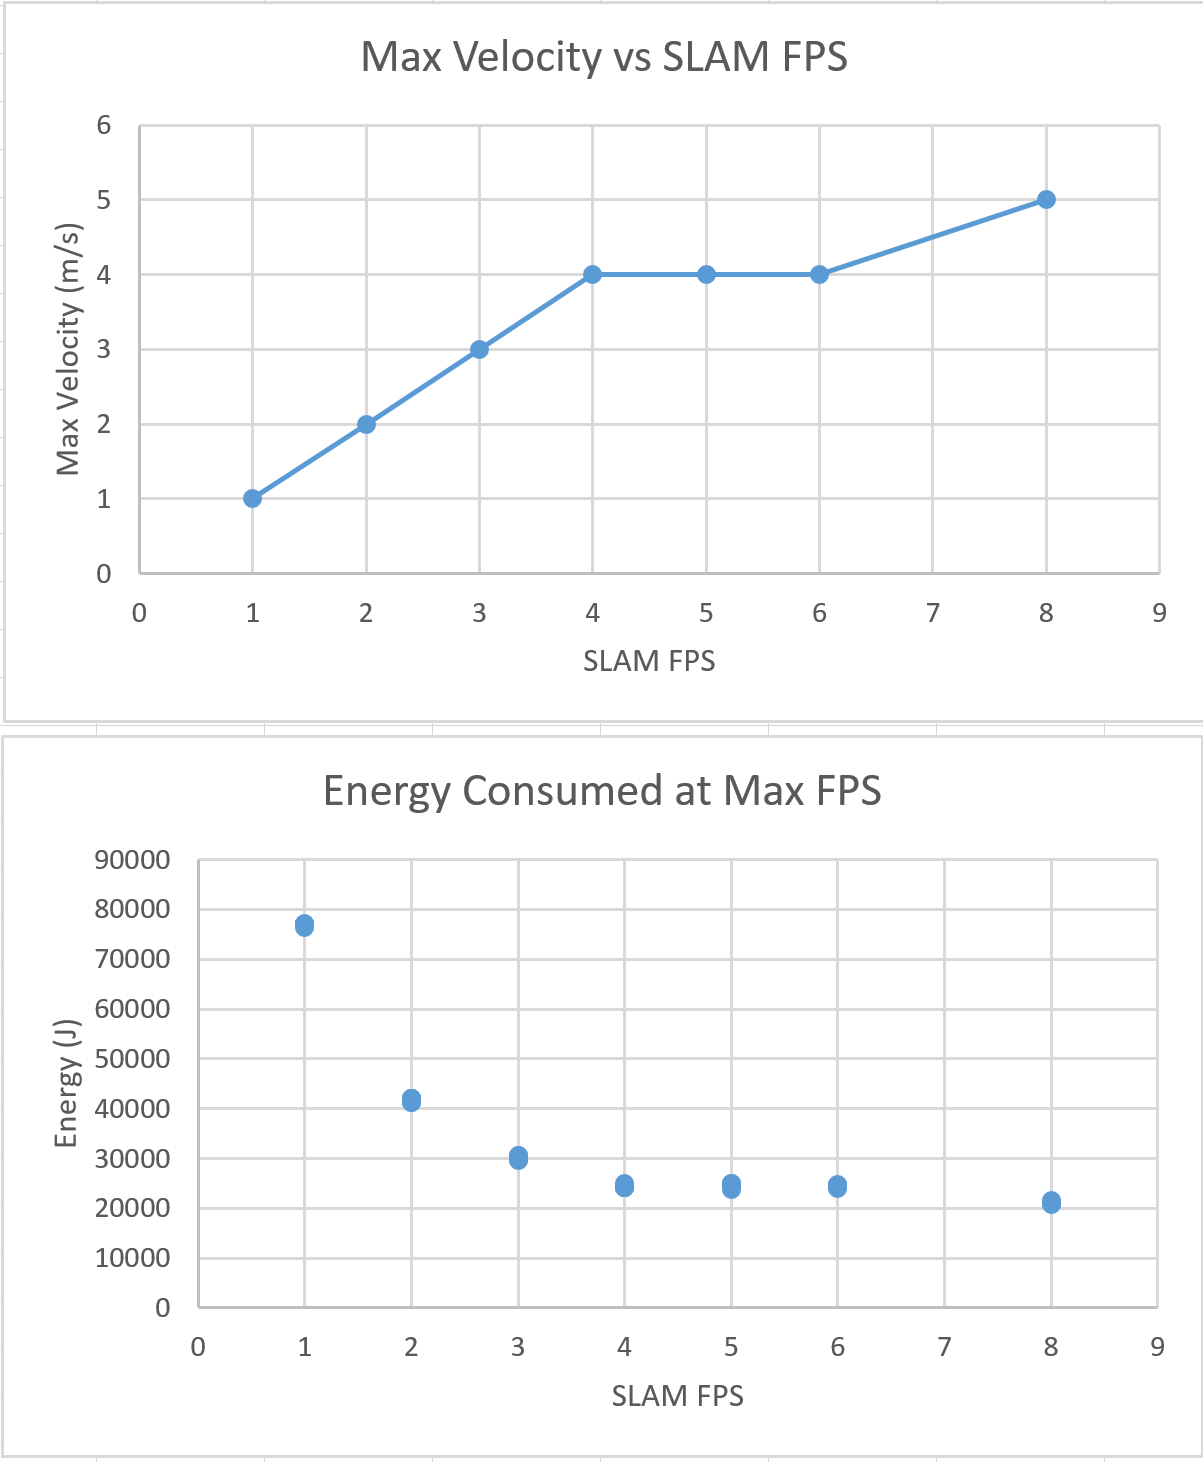
\includegraphics[width=\columnwidth]{figs/slam-speed-energy.png}
\caption{relationship between drone's speed compute power}
\label{sec:powerbreakdown}
\end{figure}
\end{comment}
\begin{comment}
\begin{figure}[h]
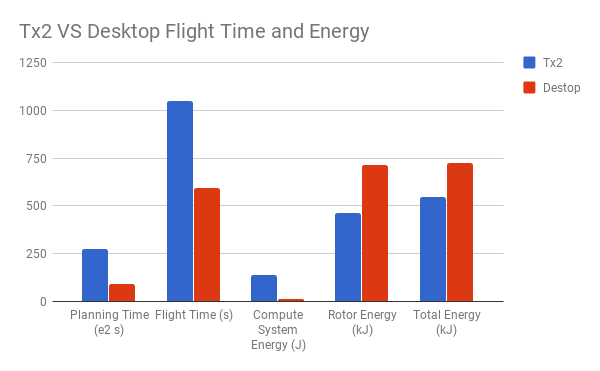
\includegraphics[width=\columnwidth]{figs/desktop_vs_tx2_mapping.png}
\caption{relationship between motion planning performance and compute power}
\label{microbenchmark_1}
\end{figure}
\end{comment}
\section{The Role of Compute in MAVs}
\label{sec:char}

In this section, we discuss how compute affects MAV systems. At the high level, compute plays a crucial role both in the overall mission time and total energy consumption of such systems. First, we discuss each effect by providing relevant  theoretical background and supplement the discussion with a microbenchmark. Then, we analyze MAVBench as a set of representative applications in which such effects can manifest.   %Figure~\ref{fig:benchmarks_data_flow} and our benchmark suits and  discuss the high level insights into aerial agents bottlenecks and their corresponding implications. 


%thout the loss of generality we use our benchmark suit to conduct studies. The results and the flow presented in section blah to explain the corresponding  the by a discussion of  total system, i.e. locomotion and compute energy consumption, and its distribution. Then, we provide case studies showing that more compute can result in an improvement in the overall system's energy consumption. Finally we delve into our application benchmark suit to discuss how such a role can effect them.

%\subsection{Compute and Accuracy Relationship}
%explain slam and present the microbenchmark

\subsection{Compute and Flight Time Relationship}

Compute can play an important role in reducing the drone's mission time by increasing the mission's average velocity. Concretely, we identify that the reduction in hover time and the increase in maximum allowed velocity are the two major ways with which more compute can contribute to a higher average velocity. Here, we shed light on these different ways.

\paragraph{Hover Time Reduction:} Hover time and the average velocity have an inverse relationship, namely, the more drone spends time on hovering, the lower its average velocity. Similar to an idling CPU, a hovering drone is unfavorable since it is not working toward its mission, but yet wasting its limited energy. A hovering drone typically is waiting for its mission planning stage to make a decision (e.g. deciding on a path to follow). \emph{More compute power can help reduce hovering (e.g by reducing the decision making time),} hence decreasing the negative effect hovering has on the average velocity. 
\begin{figure}[t!]
\centering
    \begin{subfigure}{.49\columnwidth}
    \centering
    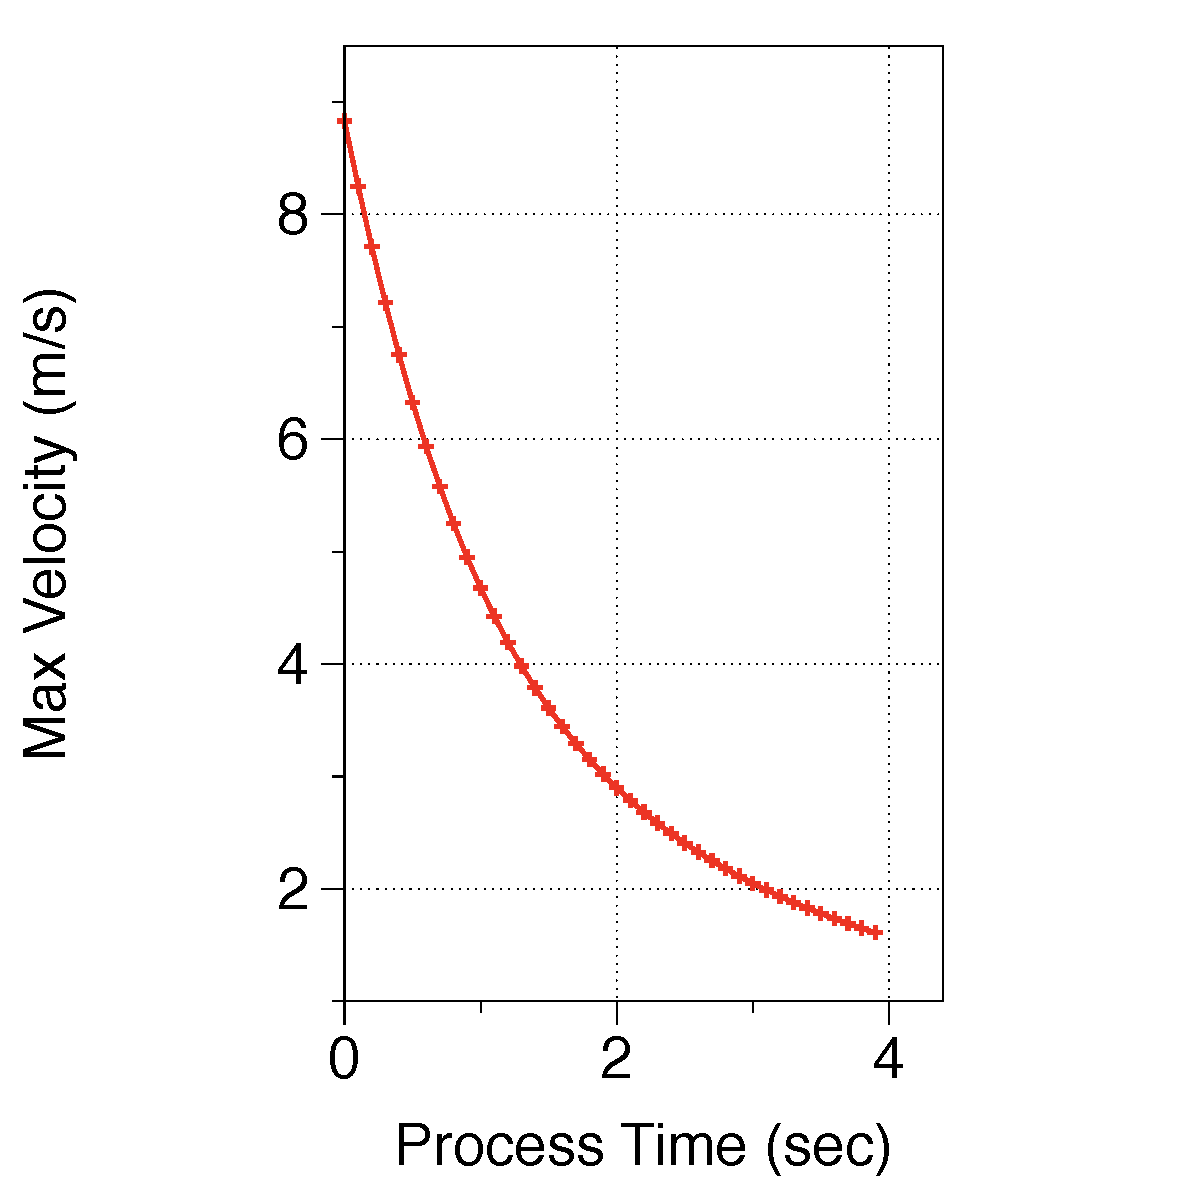
\includegraphics[trim=0 0 0 0, clip, width=1.0\columnwidth]{figs/fig_13}
    \caption{Theoretical max velocity.}
    \label{fig:process-time-velocity}
    \end{subfigure}
    \begin{subfigure}{.49\columnwidth}
    \centering
   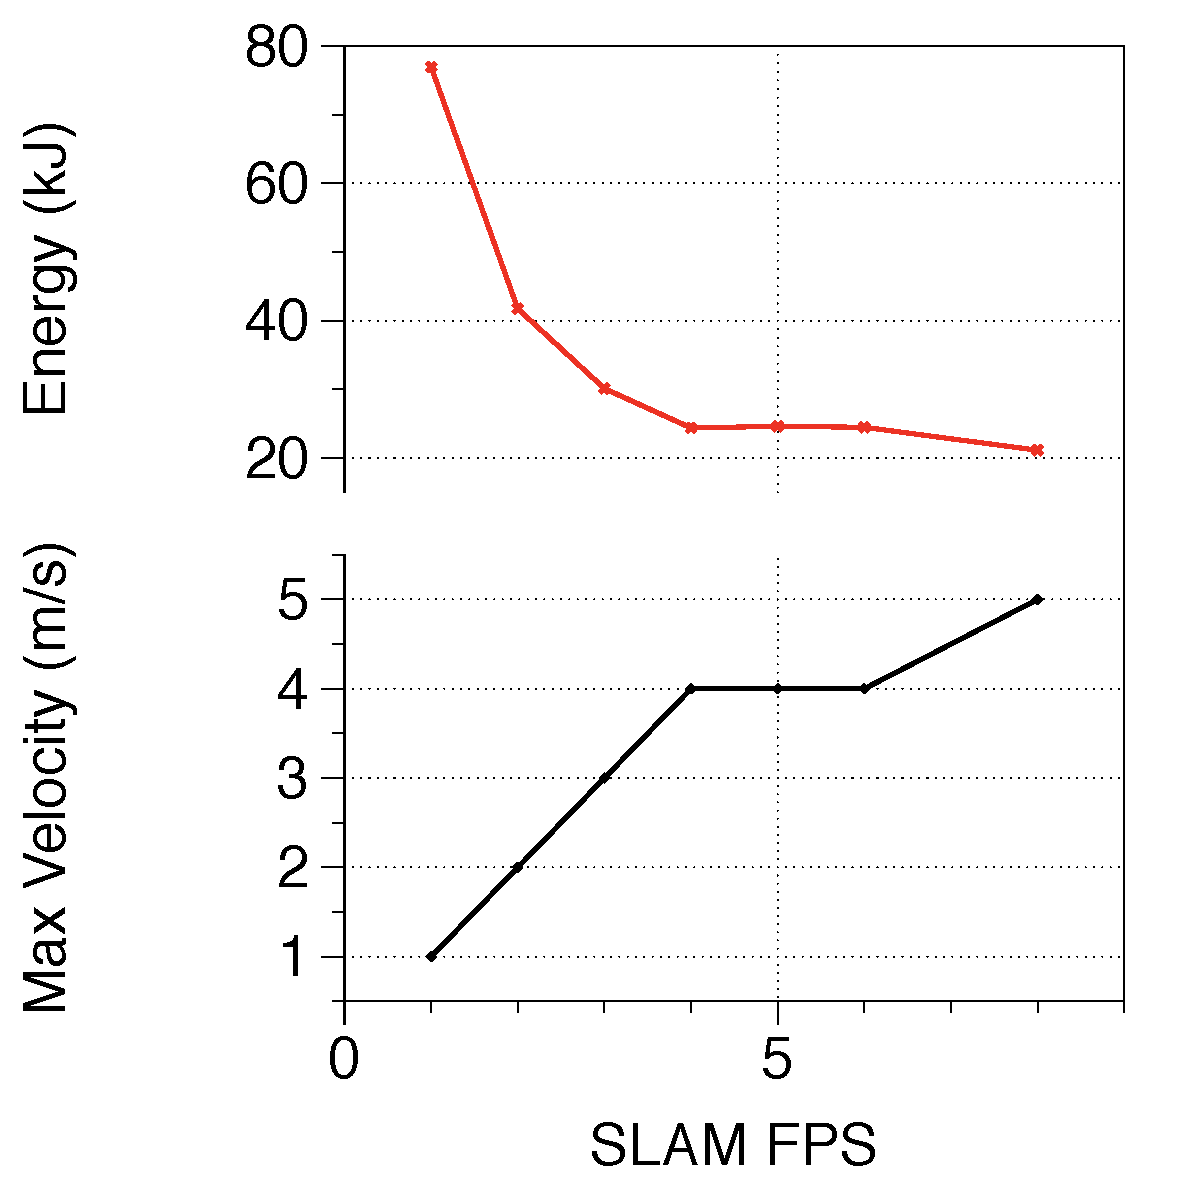
\includegraphics[trim=0 0 0 0, clip, width=1.0\columnwidth]{figs/slam_fps_velocity_energy}
    \caption{Measured max velocity.}
    \label{fig:slam-velocity-energy}
    \end{subfigure}
\vspace{-5pt}
%\setlength{\belowcaptionskip}{-4ex}
\caption{\emph{(a)} Theoretical relationship between processing time and maximum velocity. \emph{(b}) Relationship between SLAM throughput (FPS) and maximum velocity and energy of UAVs.}
%\label{SOLO_power_breakdown}
\end{figure}

\paragraph{Max Velocity Increase, Collision Avoidance Effect:} The maximum velocity of the drone is not only mechanically bounded, but also compute bounded. For a given flight velocity, a collision-free flight is only possible if the drone can process its surrounding fast enough to react to it. Therefore, \emph{a higher velocity requires a faster processing capability}. The collision avoidance task can be rather compute intensive exercising various stages of the pipeline starting from the pixel processing in the perception stage and ending with the command issue in control. In order to guarantee collision avoidance, a  drone's maximum velocity is determined based on the aforementioned pixel to response time. Equation~\ref{eq:runtime-compute-bound} specifies the components involved in setting this velocity where $\delta_{t}$, d, $a_{max}$ and v denote process time, required stopping distance, maximum acceleration limit of the drone and maximum velocity~\cite{high-speed-nav}. As \Fig{fig:process-time-velocity} shows, our simulated drone, in theory, is bounded by the max velocity anywhere between 8.83 to 1.57 m/s given a pixel to response time of the range 0 to 4~seconds. 

\begin{comment}
\begin{figure}[t]
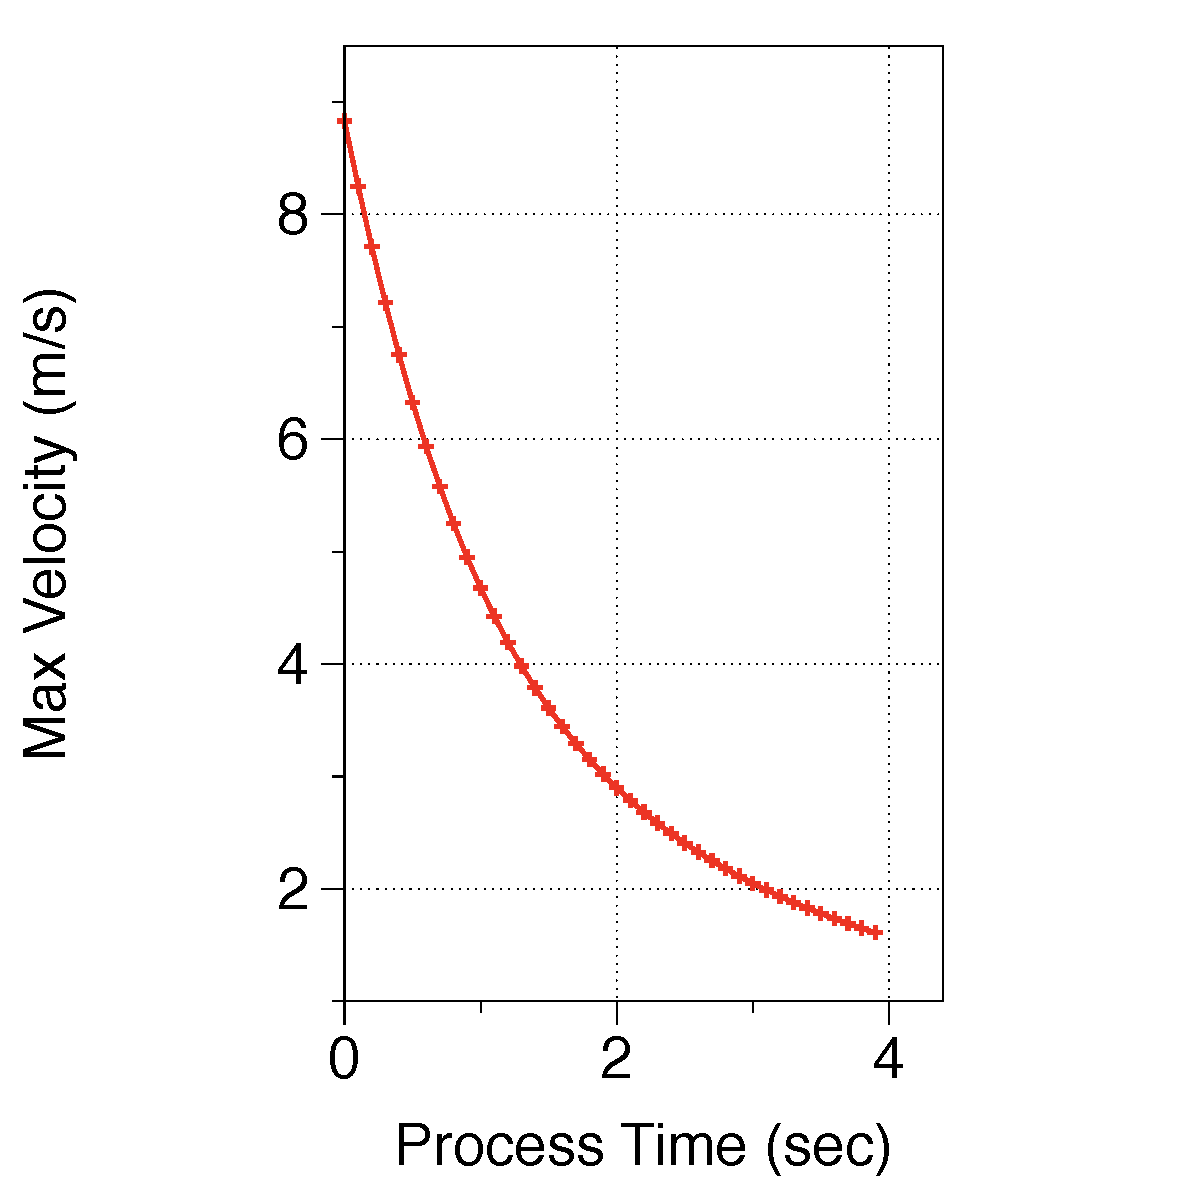
\includegraphics[width=\columnwidth]{figs/fig_13}
\caption{Theoretical relationship between process time and max velocity}
\label{sec:vel_proc_relationship_figure}
\end{figure}
\end{comment}

\begin{equation}
\label{eq:runtime-compute-bound}
v_{max} = a_{max}(~\sqrt[]{\delta{t}^2 + 2\frac{d}{a_{max}}} - \delta{t})
\end{equation}
\setlength{\belowcaptionskip}{-1ex}

\paragraph{Max Velocity Increase, Localization Failure Effect:} The faster the speed of the drone, the higher the likelihood of its localization failure because the environment changes rapidly around a fast drone. Kernels such as SLAM which help localize the drone by tracking a set of points/features through successive camera frames struggle to keep up with the rate of these changes. It is important to note that localization failures can have catastrophic effects such as permanent loss or spending of extra time (for example by backtracking) for re-localization. 

Minimizing or avoiding localization related failure scenarios is highly favorable, if not necessary. To examine the relationship between the compute, maximum velocity and localization failure, we devised a micro-benchmark in which the drone was tasked to follow a predetermined circular path of the radius 25~meters. For the localization kernel, we used ORB-SLAM2 and to emulate different compute powers, we inserted a sleep in the kernel. We swept different velocities and sleep times and bounded the failure rate to 20\%. As \Fig{fig:slam-velocity-energy} shows, higher FPS values, i.e. more compute, allows for a higher maximum velocity for a bounded failure rate. 

%\begin{figure}[h]
%\includegraphics[]{figs/blank.pdf}
%\caption{Measurement set up to collect power data for 3DR Solo.}
%\label{sec:powerbreakdown}
%\end{figure}
\begin{figure}[!t]
\centering
    \begin{subfigure}{.49\columnwidth}
    \centering
    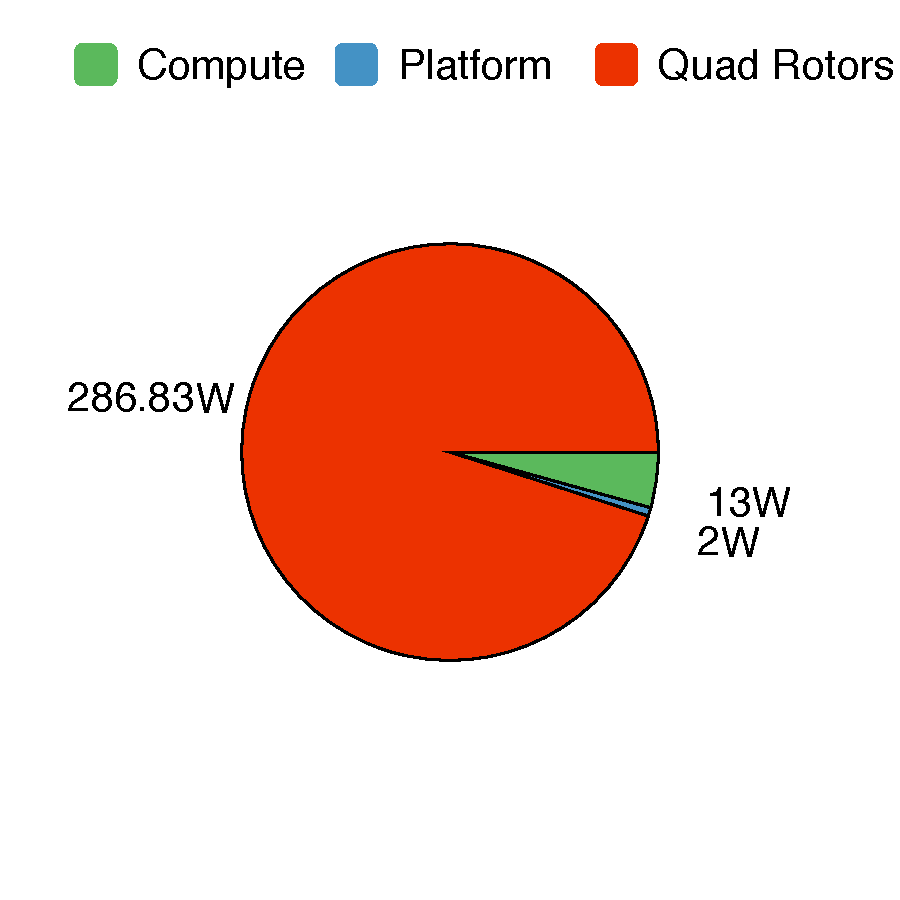
\includegraphics[trim=0 0 0 0, clip, width=1.0\columnwidth]{figs/power_break_down_tx2}
    \caption{Measured power breakdown.}
    \label{fig:SOLO-power-breakdown}
    \end{subfigure}
    \begin{subfigure}{.49\columnwidth}
    \centering
    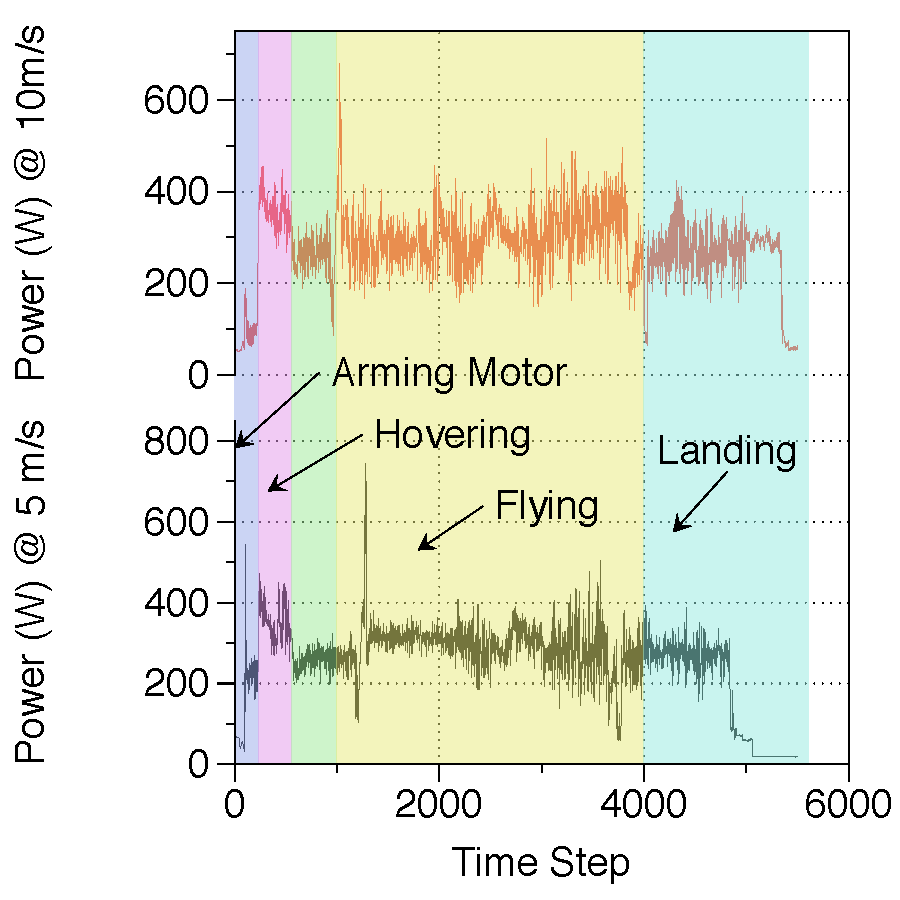
\includegraphics[trim=0 0 0 0, clip, width=1.0\columnwidth]{figs/drone-power-time-series}
    \caption{Measured mission power.}
    \label{fig:drone-power-time-series}
    \end{subfigure}
\caption{\emph{(a)} Measured power consumption of a flying 3DR Solo. \emph{(b)} Total measured power consumption while the drone is "Flying" at two different steady-state velocities. The power consumption is severely dominated by the quad rotors by 20X.}
\label{SOLO_power_breakdown}
\end{figure}
\subsection{Compute and Energy Relationship}
The compute subsystem can also have a significant role in reducing total MAV energy consumption. To understand this, first we present the power distribution associated with \solo~\cite{solo3DR}, a popular off-the-shelf MAV. To measure power, we attach a wattmeter known as Eagle~Tree Systems eLogger~V4~\cite{eLoggerV4} to the \solo's battery during flight. The wattmeter allows us to collect data over time at 50~Hz while the drone flies. We command the drone to fly for fifty seconds and pull the data off of the wattmeter after the drone lands.

% The wattmeter gave us the total power consumed by the drone, without a deeper breakdown. To estimate the portion of the instantaneous power that would typically be consumed by a MAV's processor, we subtracted the idle power consumption of the \solo's default on-board computer and added to it the power consumed by the TX2 during typical workloads.

As \Fig{SOLO_power_breakdown} shows, the majority of the power consumption is dedicated to rotors (locomotion) and the compute only occupies a small portion of the entire pie and its role seemingly trivial. Although small in quantity, compute can have a grand effect on the system's power. This is because by reducing the mission time (as explained in the previous section), more compute power can, in fact, reduce the bigger portion of the pie, namely rotors energy consumption (due to a shorter flight). Note that although more compute can lead to more energy consumption of the compute subsystem, the reduction in rotor's energy can easily outweigh such an increase.  
% \setlength{\belowcaptionskip}{-2ex}


We profiled the mission time and the energy associated with the aforementioned microbenchmark. As the bottom plot in \Fig{fig:slam-velocity-energy} shows, higher compute capability results in increased SLAM FPS and hence a reduction in mission time by allowing for faster velocity. The reduced mission results in reduced total system energy, as the top plot in \Fig{fig:slam-velocity-energy} shows. By increasing processing speed by 5X, we were able to reduce the drone's energy consumption by close to 4X.

\subsection{MAVBench Workloads Compute vs. Flight Time vs. Energy}
\label{sec:operating-spoints}
We use our benchmark suite as a representative set of applications to examine the effect of compute on MAV systems. To analyze this effect, we conducted sensitivity analysis to core and frequency scaling of the TX2 board. TX2 has two sets of cores, namely a \textit{HMP Dual Denver cores} and a \textit{Quad ARM A57}. We turned off the Denver cores so that the indeterminism caused by process to core mapping variations across runs would not affect our results.
Average velocity, mission, and energy values of various operating points are profiled and presented as heat maps (\Fig{fig:benchmarks:OPA:scanning}---\Fig{fig:benchmarks:OPA:ap}) for a DJI Matrice 100 drone. \emph{In general, compute can improve mission time and lower energy consumption by as much as 5X.}

\paragraph{Scanning:}
We observe trivial differences for velocity, endurance and energy across all three operating points (\Fig{fig:benchmarks:OPA:scanning:velocity}, \Fig{fig:benchmarks:OPA:scanning:time}, and \Fig{fig:benchmarks:OPA:scanning:energy}). This is despite seeing a 3X boost in the motion planning kernel, i.e. lawn mower planning, which is its bottleneck (\Fig{fig:kernel-breakdown}). The trivial effect of compute on this application is because planning is done once at the beginning of the mission and its overhead is amortized over the rest of the mission time. For example the overhead of planning for a 5 minute flight is less than .001\%.  
%\vspace{2pt}

%We present our understanding and takeaways regarding the computational bottlenecks and the effect of compute on them.


%Each application and its associated nodes are time profiled (table~\ref{kernel_makeup}).  We use this table along with the data flow presented in figure    \label{fig:benchmarks} to dissect and understand various compute bottlenecks. 

%At the high level, each application contains a node called mission planner responsible for high level decision making and arbitrating flight command issuance. When needed, this nodes place a service call to the motion planning kernel, setting out drones next set of moves. Some of our applications have the collision avoidance capability. This node exercises all stages of the pipeline starting from the perception stage, i.e. point cloud generation, OctoMap, collision check, to planning, mission planner/motion planner and ending with control, i.e. path tracking/command issue. 

 
%and their kernel makeup is provided. This will help us to understand the bottle-necks and opportunities for improvements.

%It would be wise to note that this application is intentionally design minimally without an involved perception and planning because ~\red{ask vijay. He knows very well how to justify this}.

\paragraph{Package Delivery}:  As compute scales with the number of cores and/or frequency values, we observe a reduction of up to 84\% and 82\% for the mission time and energy consumption, respectively (\Fig{fig:benchmarks:OPA:pd:time}, and \Fig{fig:benchmarks:OPA:pd:energy}). The sequential bottlenecks i.e. motion planning and OctoMap generation kernel are sped up by frequency scaling to enable the observed improvements. There does not seem to be a clear trend with core scaling, concretely between 3 and 4 cores. We conducted investigation and determine that such anomalies are caused by the non-real-time aspects of ROS, AirSim and the TCP/IP protocol used for the communication between the companion computer and the host. We achieve up to 2.9X improvement in OctoMap generation and that leads to maximum velocity improvement. It is important to note that although we also gain up to 9.2X improvements for the motion planning kernel, the low number of re-plannings and its short computation time relative to the entire mission time render its impact trivial. Overall the aforementioned improvements translate to up to 4.8X improvement in the average velocity. Therefore, mission time and the MAV's total energy consumption are reduced.

%OctoMap generation is a major computationally intensive kernel in this application. This kernels performance OctoMap is of utmost importance since it is on the collision avoidance path. As shown in the data flow, this path starts with depth images and flows through point cloud generation, OctoMap generation, collision check and finally ends in the control.  OctoMap is responsible for 99\% of the pixel to response time determined by this path. Figure blah shows how OctoMap kernel scales with different number of cores and frequencies. 

%Motion planner is another computationally intensive kernel for this application. Although at first glance, its optimization can improve the mission time, the low number of re-plannings and its short computation time relative to the entire mission time render its impact trivial. For example, if we re-plan 20 times during the coarse of 5 minutes of the mission time, planning time would only consume .01\% of the entire flight.  
 
\begin{comment}
\begin{figure}[h]
\includegraphics[width=\columnwidth]{figs/velocity_process_time_relationship}
\caption{Theoretical relationship between process time and max velocity}
\label{sec:vel_proc_relationship}
\end{figure}
\end{comment}

%lowering the process time, results in a higher velocity and in turn, lowering the mission time and energy. 
%Explain collision avoidance path and policty and then discuss how octomap and planning comprise most of the it and the rest is ros runtime overhead. 
%Our pixel to response time is equal to 1.2 seconds most of which is dedicated to octomap and planning as is showing in the table.   

%As opposed to the surveying benchmark, package delivery's trajectory is determined at the mission time.  perception of the obstacles surrounding the drone at any moment and also on the way to the destination is required. To do so, a map of once visible and visited environment is created and maintained within an octomap structure \ref{blah}. Arriving at such a map requires converting image depth information to point clouds (point cloud generation node) and integrating them to the map (octomap server). It is important to note the dynamic obstacles are intentional not captured within the octomap. Motion planner, attempts to find the shortest path to the destination with the knowledge of such map and only remap on demand. 
  
%As the drone follow its trajectory, new trajectory can be demanded due to environmental triggers. These environmental triggers can be static obstacles unaccounted for at the time of planning (since they were not in the sensor's visibility range). Dynamic obstacles not present at the time of planning can also trigger replannings. 

%These triggers are identified using the panic and the future collision node. The future collision node identifies whether an obstacle (mainly static ones) is on the trajectory planned and alarm the mission planner node to request a re-plan. Since future collision operates on octomap, dynamic obstacles can not be spotted to be reacted to. This is an intentional decision since dynamic obstacles can move out of the path.
%Panic node, alarms the drone of any obstacles that enters a virtual halo surrounding the drone by processing the point cloud. By equipping the drone with a forward and backward camera, we can avoid most obstacles\footnote{since each camera only has a FOV of 120 degree, there are blind spots for our drone. To fix this, more sensors are required. We address this issue in the limitation section}  This node is our solution to dynamic obstacles. In addition to dynamic obstacles, this node can save the drone from crashing in any obstacle if the control node (follow trajectory) allows for a drift from it's supposed trajectory. 

%Due to small number of replannings, the hover time associated with the planning stage has a minor affect on the mission time. In addition, small time associated with real time threads such as panic and future collision does not demand more attention. Hence, compute's role on this application is minor.

{
\begin{figure}[t!]
    	\centering
    	\begin{subfigure}[t!]{.3\columnwidth}
    	\centering
    		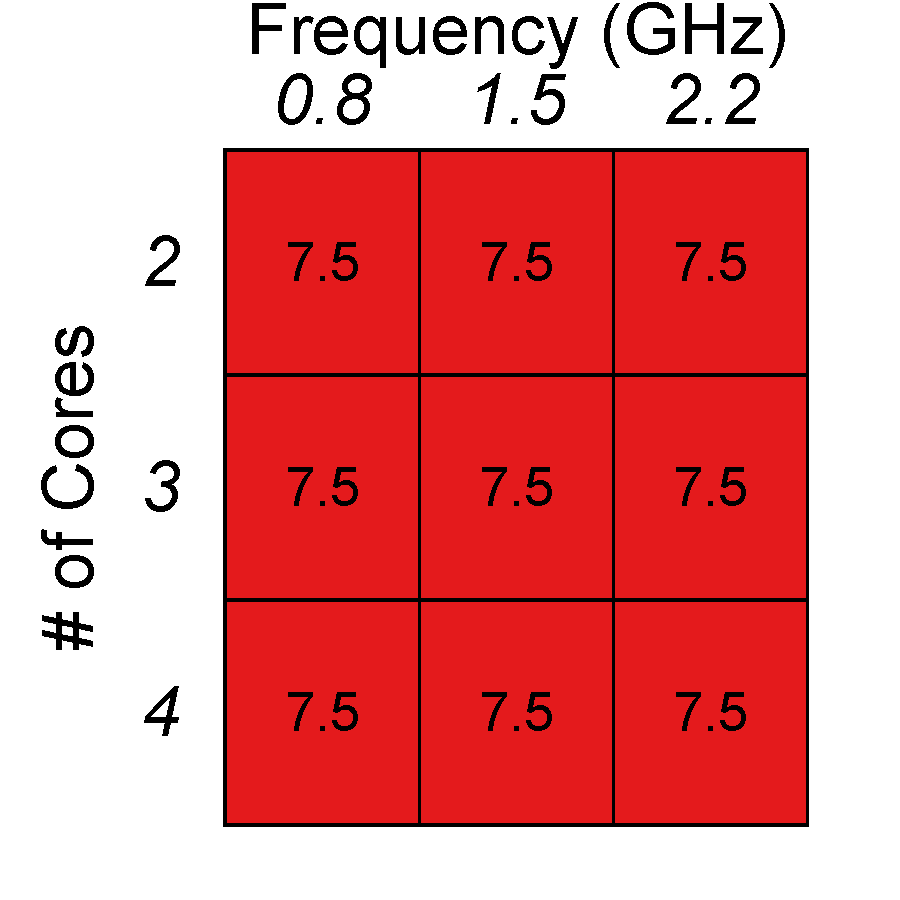
\includegraphics[width=\columnwidth]{figs/scanning_velocity_operating_point}
    		\caption{Velocity (m/s)}
            \label{fig:benchmarks:OPA:scanning:velocity}
    	\end{subfigure}
        \begin{subfigure}[t!]{.3\columnwidth}
    	\centering 
    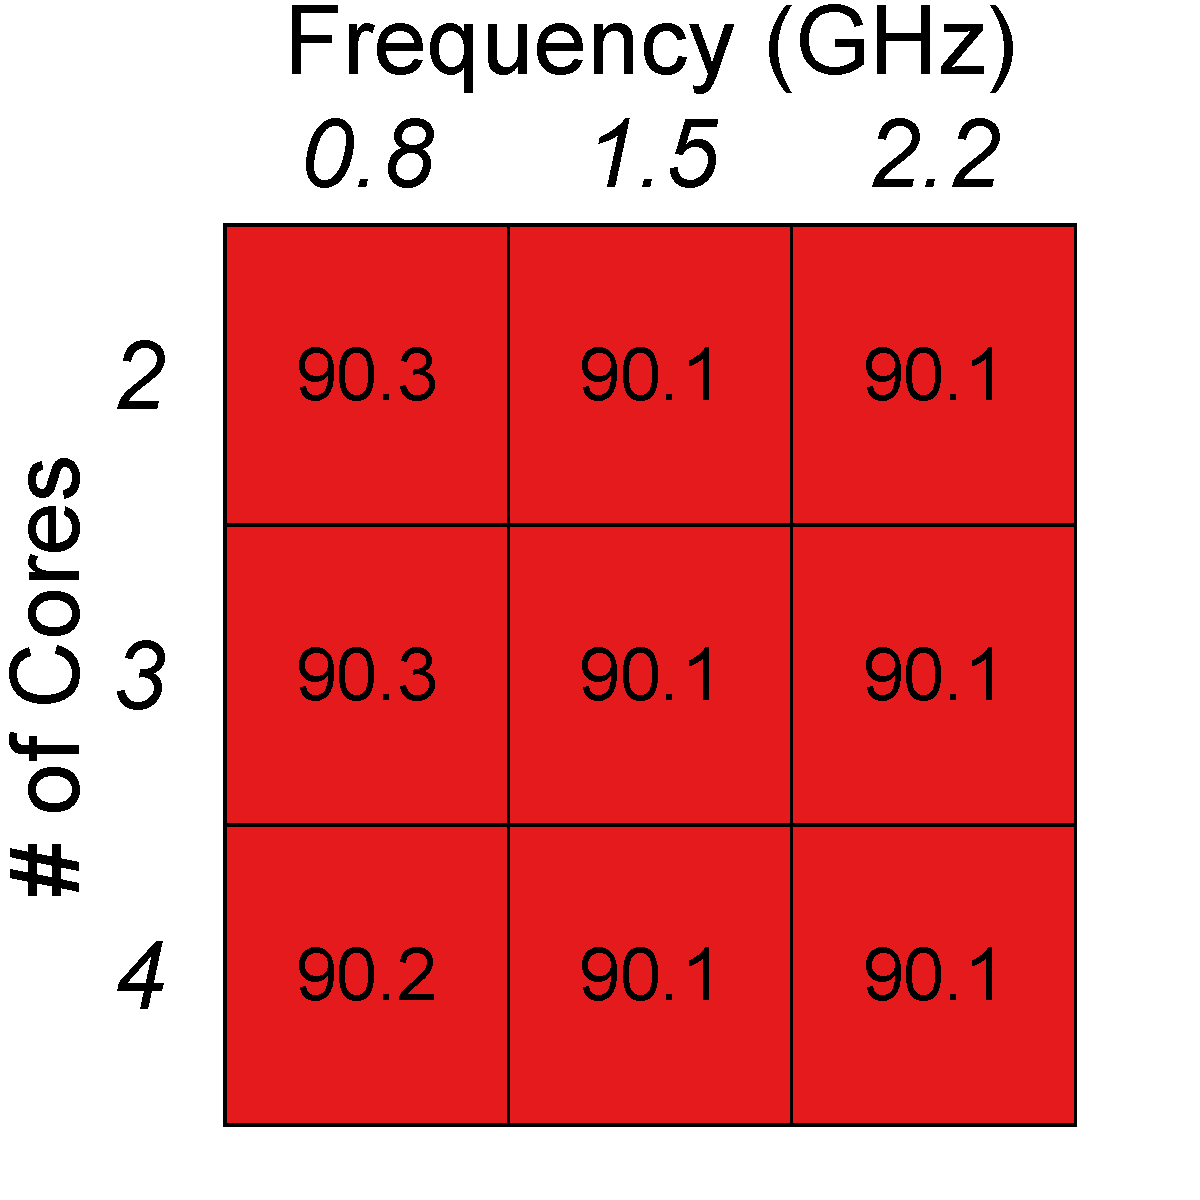
\includegraphics[width=\columnwidth]{figs/scanning_flight_time_operating_point}
    \caption{Mission Time (s)}
    \label{fig:benchmarks:OPA:scanning:time}
    \end{subfigure}
    \begin{subfigure}[t!]{.3\columnwidth}
    \centering
    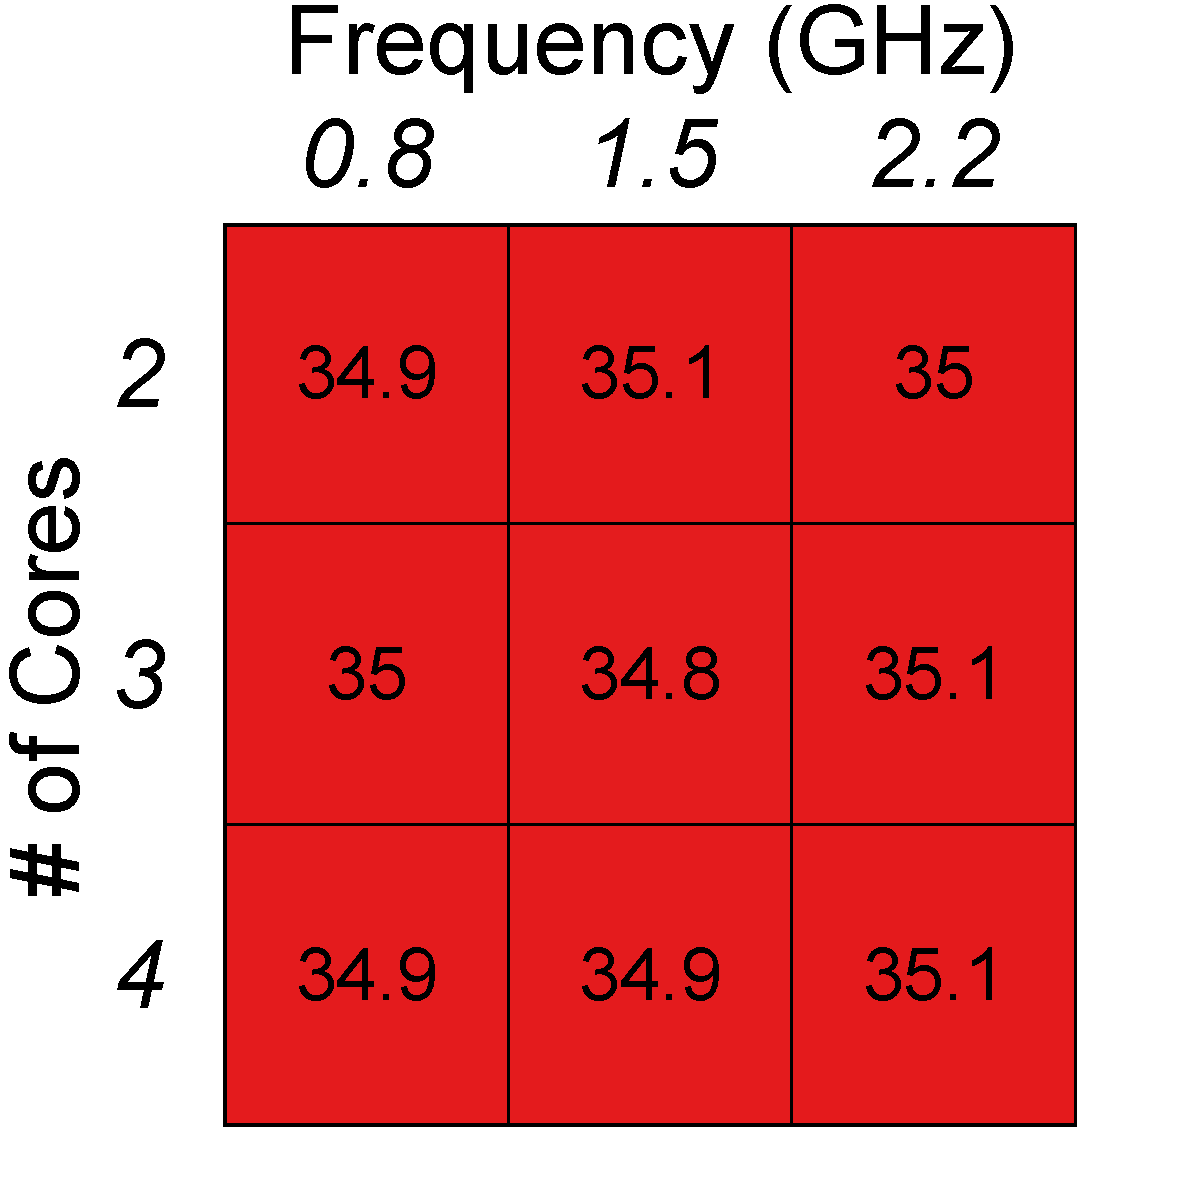
\includegraphics[width=\columnwidth] {figs/scanning_energy_operating_point}
    \caption{Energy (kJ)}
    \label{fig:benchmarks:OPA:scanning:energy}
    \end{subfigure}
    \caption{Scanning.}
    \label{fig:benchmarks:OPA:scanning}
    \end{figure}%
   \begin{figure}[t!]
    \centering
    \begin{subfigure}[t!]{.3\columnwidth}
    \centering
    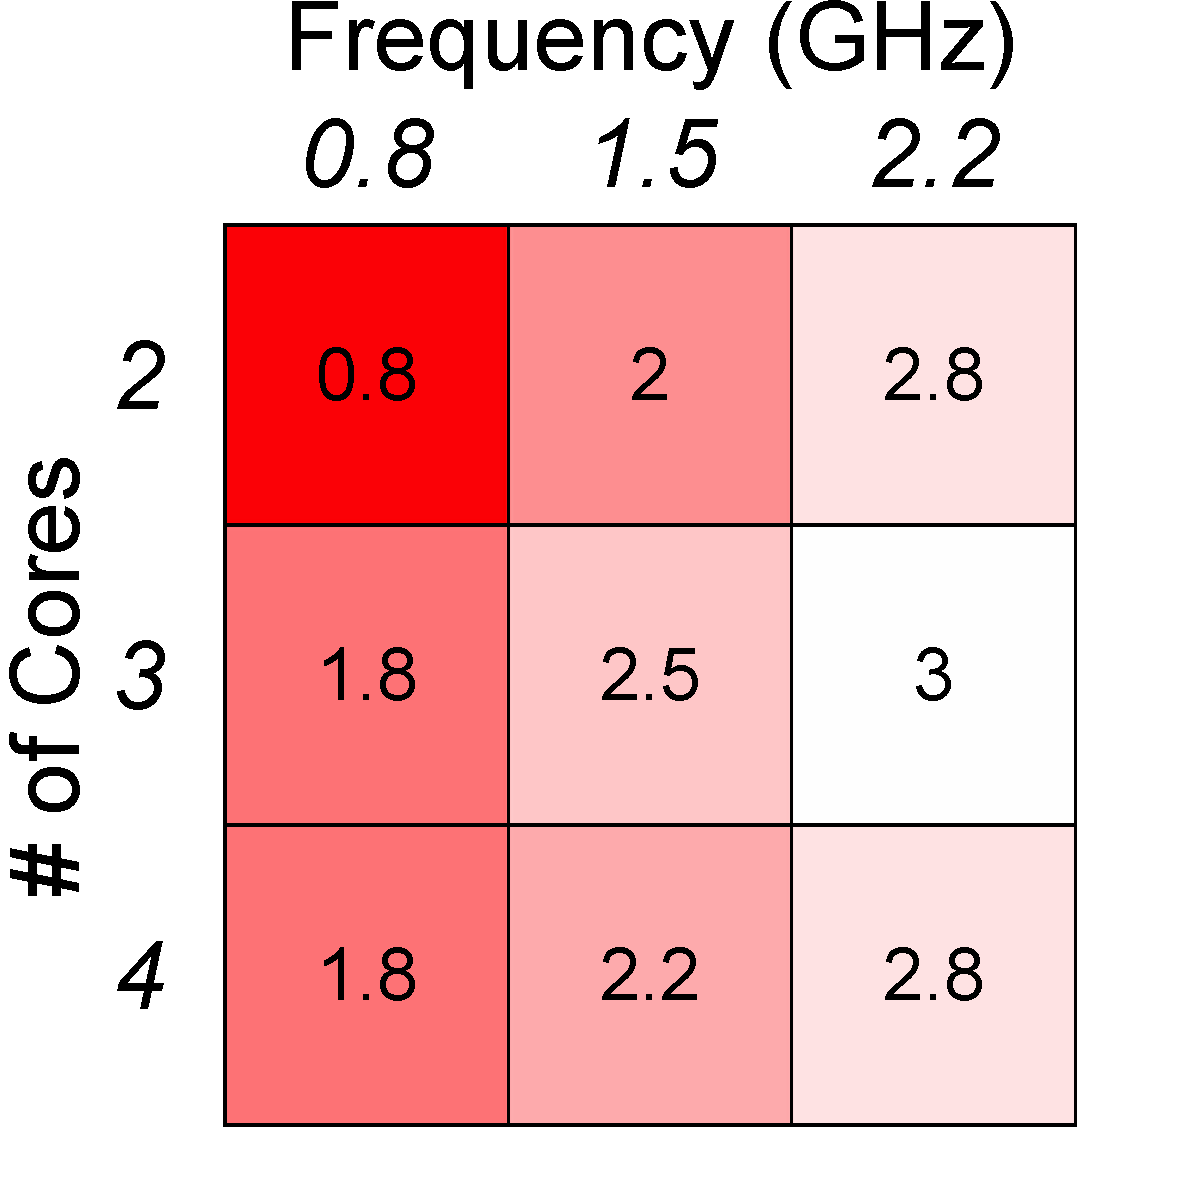
\includegraphics[width=\columnwidth]{figs/pd_velocity_operating_point}
    \caption{Velocity (m/s)}
     \label{fig:benchmarks:OPA:pd:velocity}
    \end{subfigure}
    \begin{subfigure}[t!]{.3\columnwidth}
    \centering
    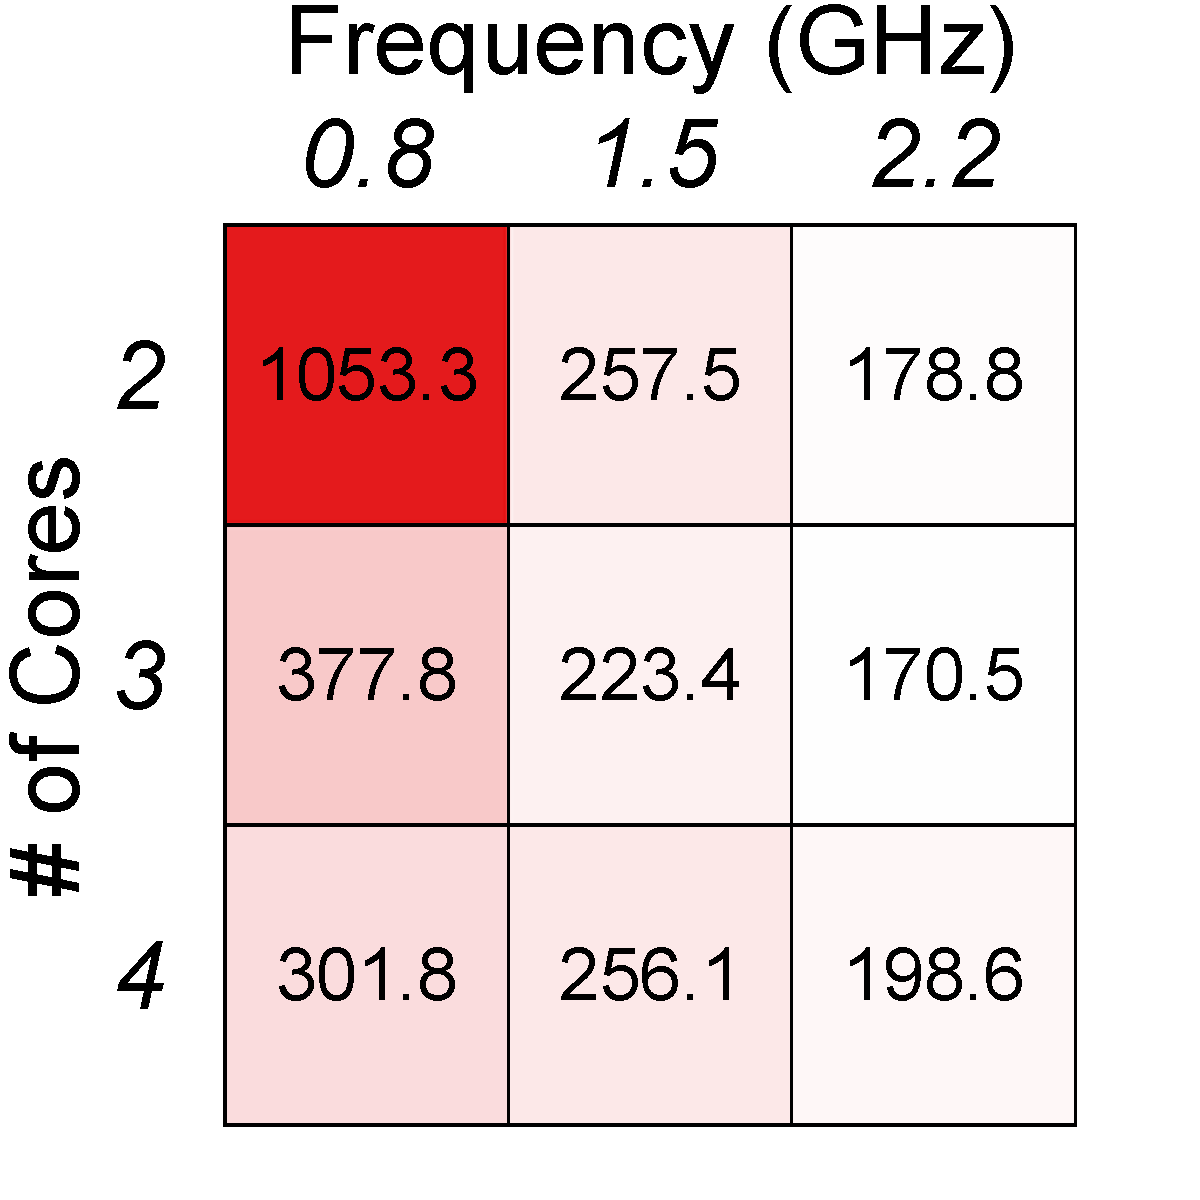
\includegraphics[width=\columnwidth]{figs/pd_flight_time_operating_point}
    \caption{Mission Time (s)}
    \label{fig:benchmarks:OPA:pd:time}
    \end{subfigure}
    \begin{subfigure}[t!]{.3\columnwidth}
    \centering
    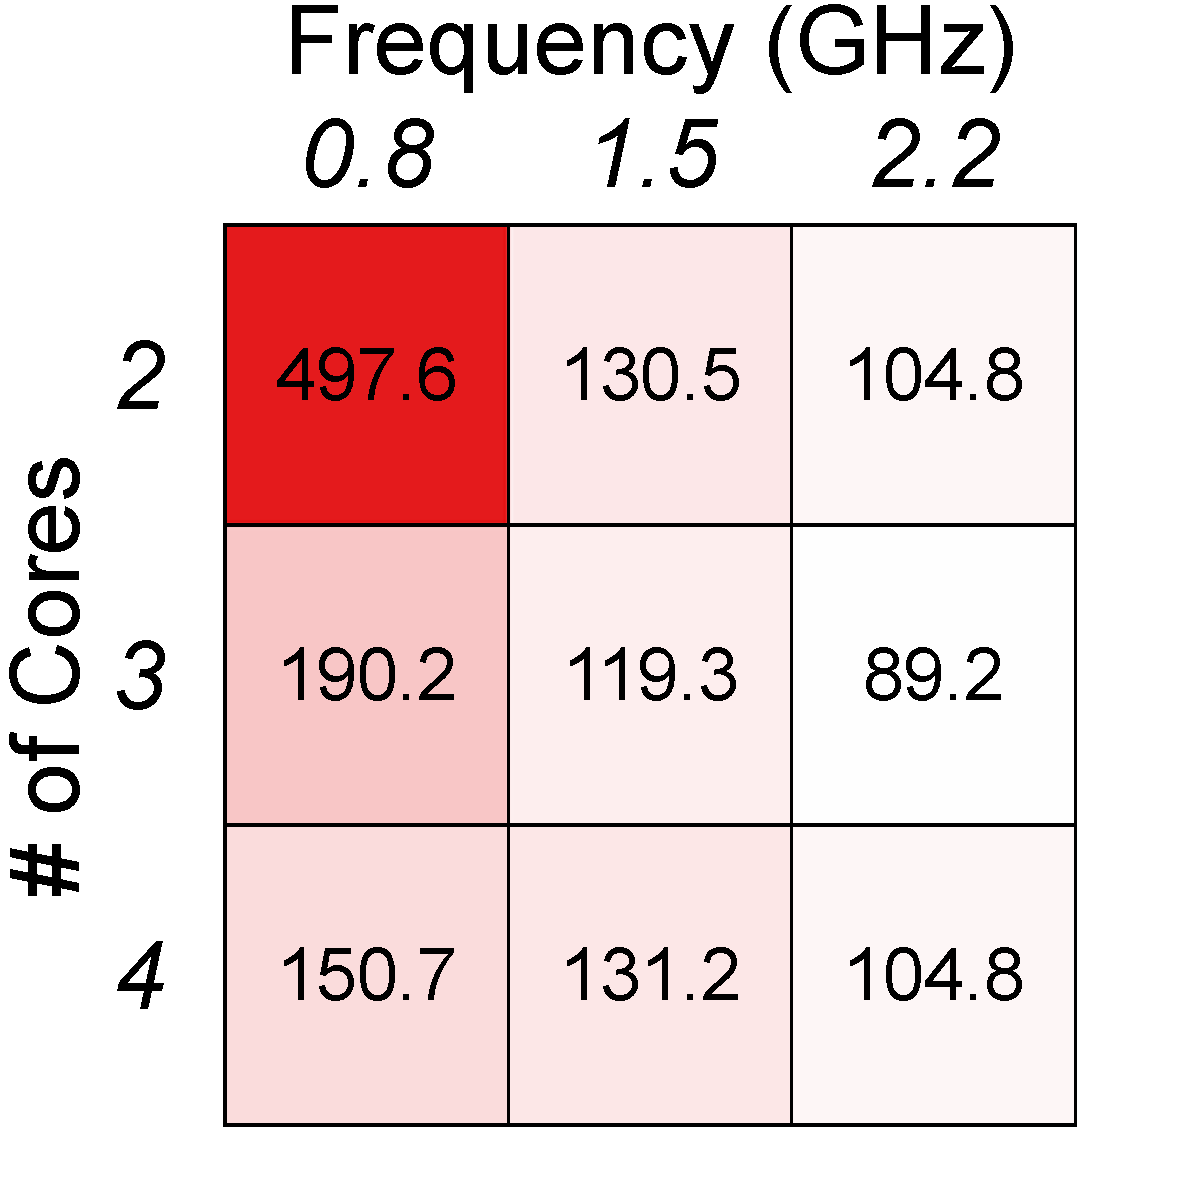
\includegraphics[width=\columnwidth] {figs/pd_energy_operating_point}
    \caption{Energy (kJ)}
     \label{fig:benchmarks:OPA:pd:energy}
    \end{subfigure}
    \caption{Package Delivery.}
    \label{fig:benchmarks:OPA:pd}
    \end{figure}%
    \begin{figure}[t!]
    \centering
    \begin{subfigure}[t!]{.3\columnwidth}
    \centering
    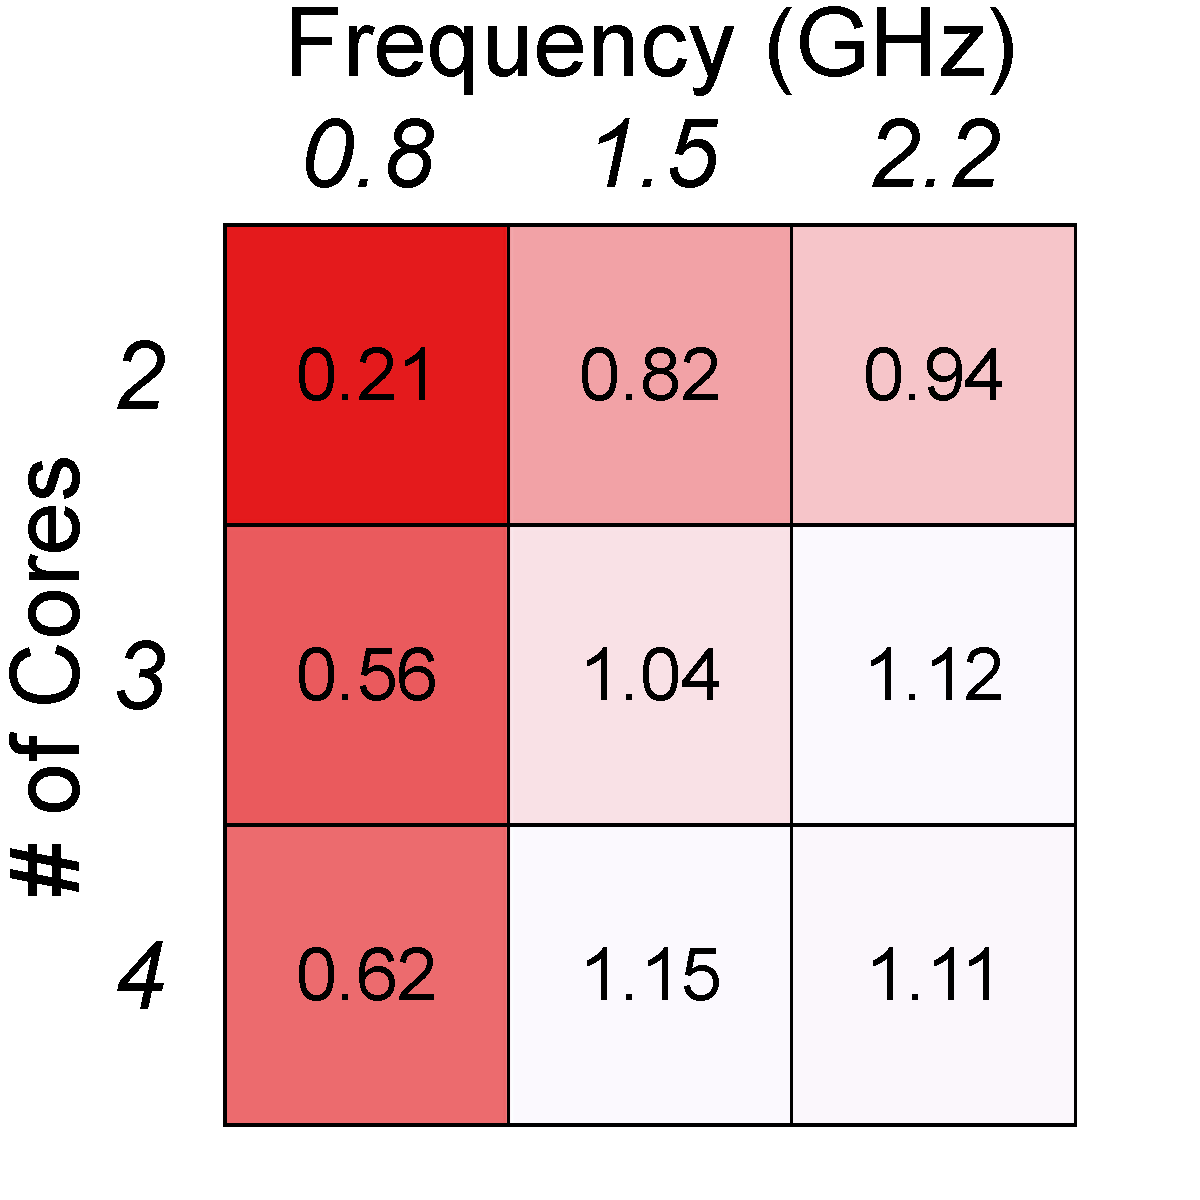
\includegraphics[width=\columnwidth]{figs/mapping_velocity_operating_point}
    \caption{Velocity (m/s)}
     \label{fig:benchmarks:OPA:mapping:velocity}
    \end{subfigure}
    \begin{subfigure}[t!]{.3\columnwidth}
    \centering
    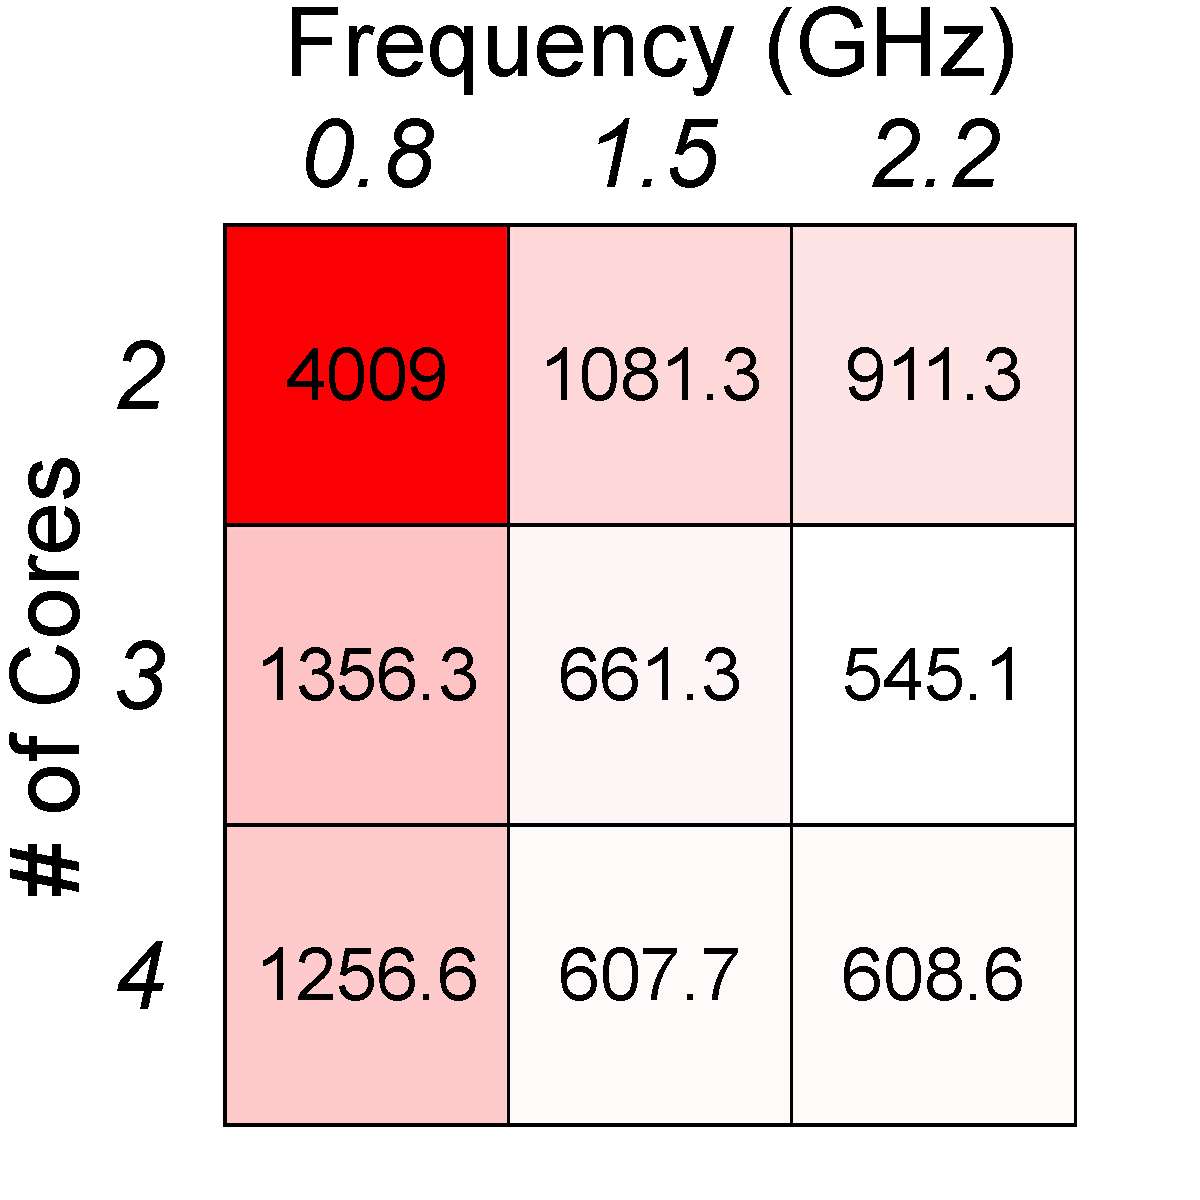
\includegraphics[width=\columnwidth]{figs/mapping_flight_time_operating_point}
    \caption{Mission Time (s)}
    \label{fig:benchmarks:OPA:mapping:time}
    \end{subfigure}
    \begin{subfigure}[t!]{.3\columnwidth}
    \centering
    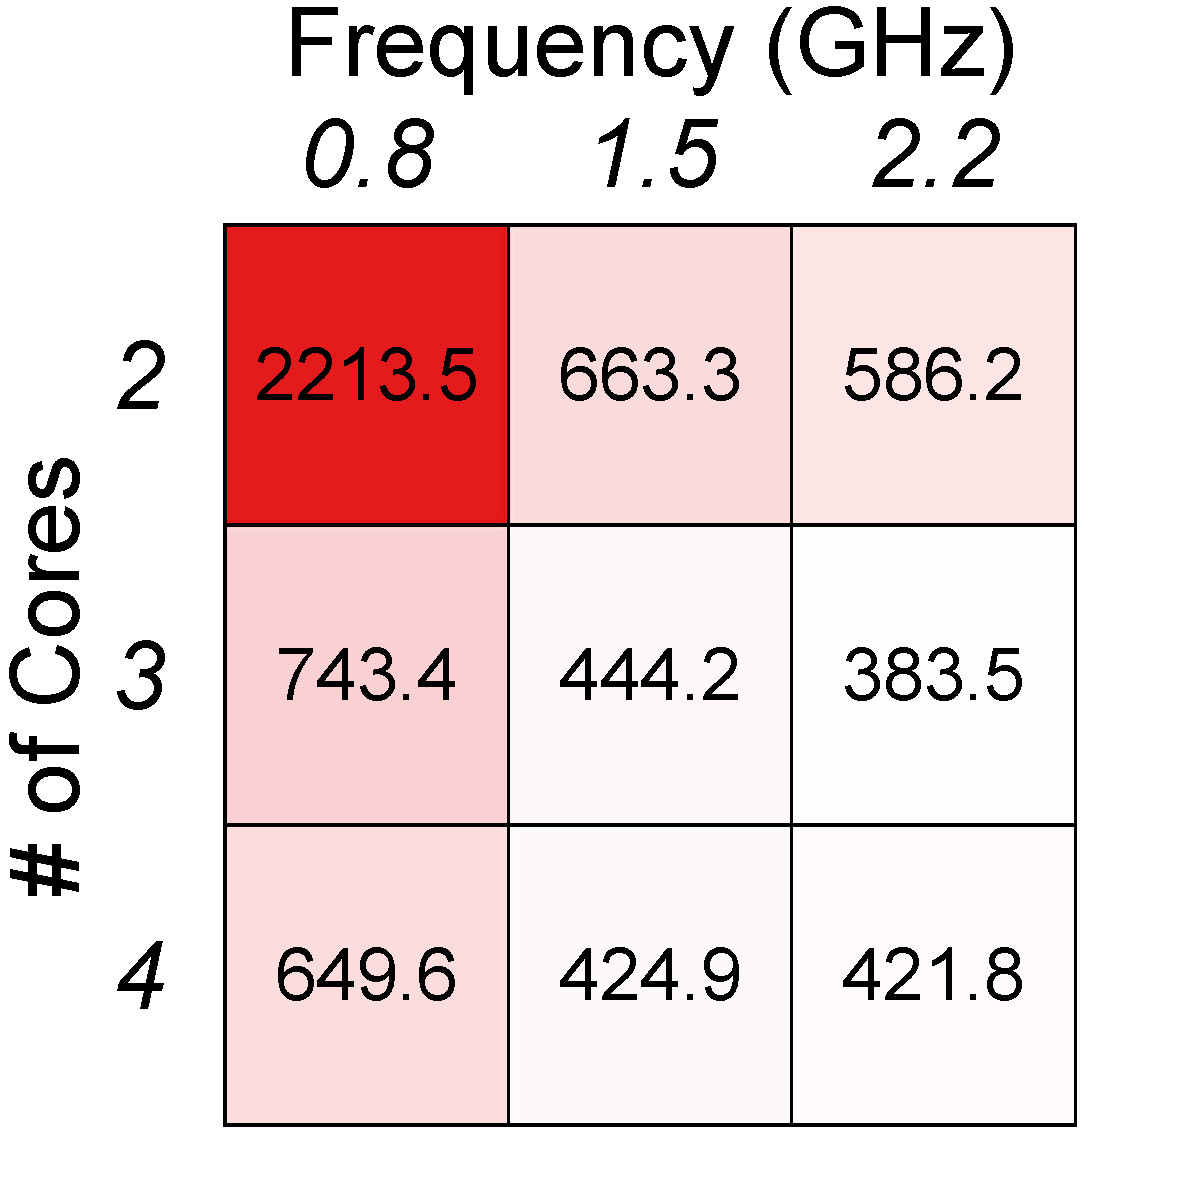
\includegraphics[width=\columnwidth] {figs/mapping_energy_operating_point}
    \caption{Energy (kJ)}
     \label{fig:benchmarks:OPA:mapping:energy}
    \end{subfigure}
    \caption{Mapping.}
    \label{fig:benchmarks:OPA:mapping}
    \end{figure}%
    \begin{figure}[t!]
    \centering
    \begin{subfigure}[t!]{.3\columnwidth}
    \centering
    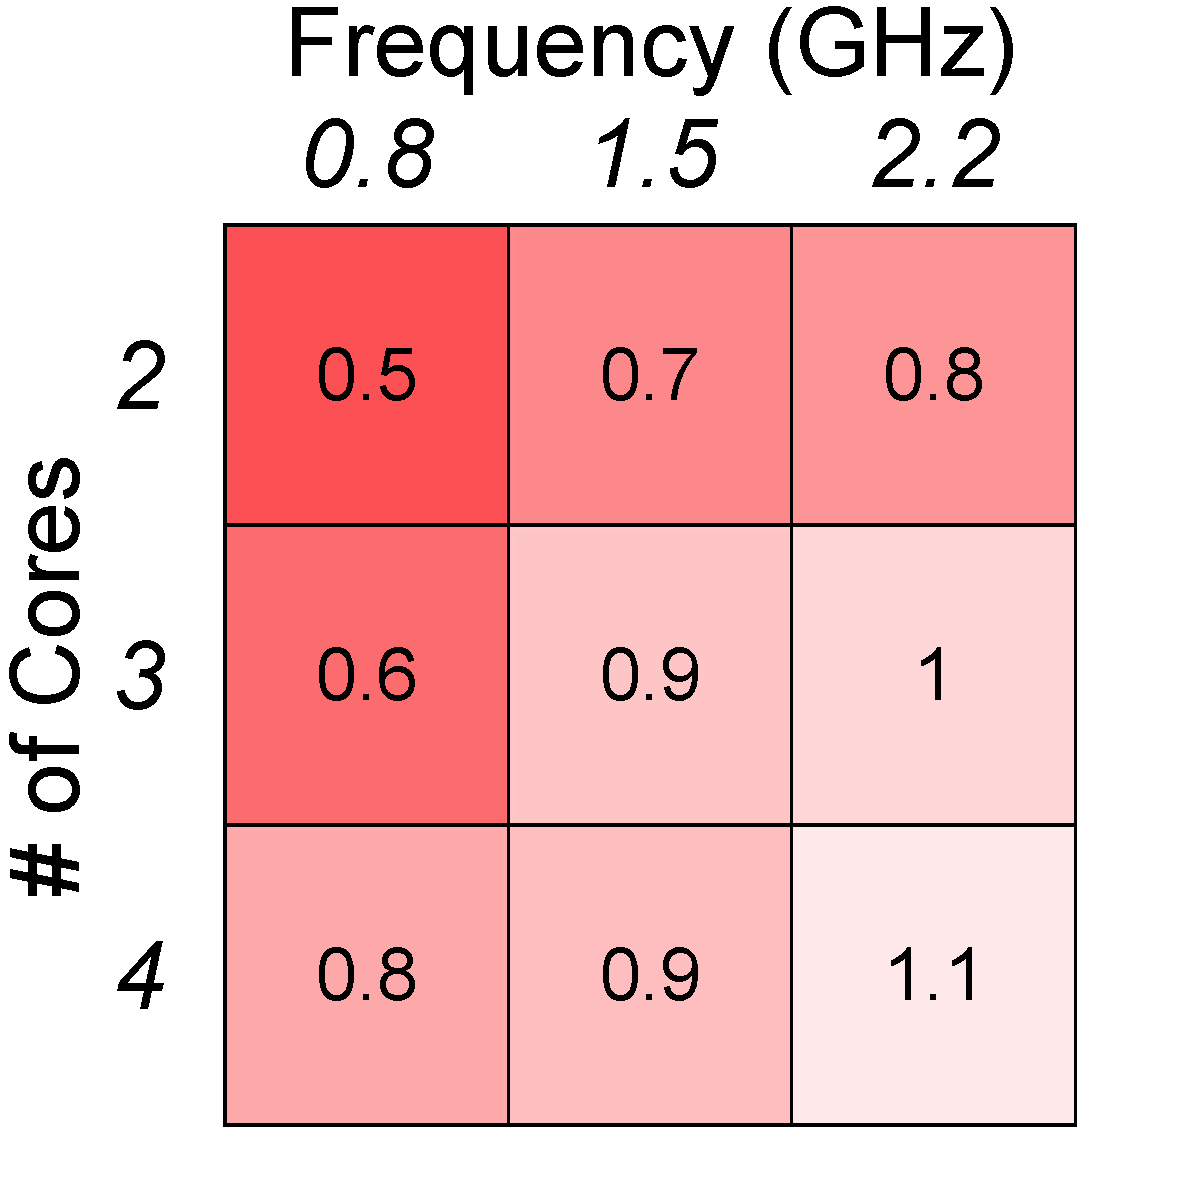
\includegraphics[width=\columnwidth]{figs/SAR_velocity_operating_point}
    \caption{Velocity (m/s)}
     \label{fig:benchmarks:OPA:sar:velocity}
    \end{subfigure}
    \begin{subfigure}[t!]{.3\columnwidth}
    \centering
    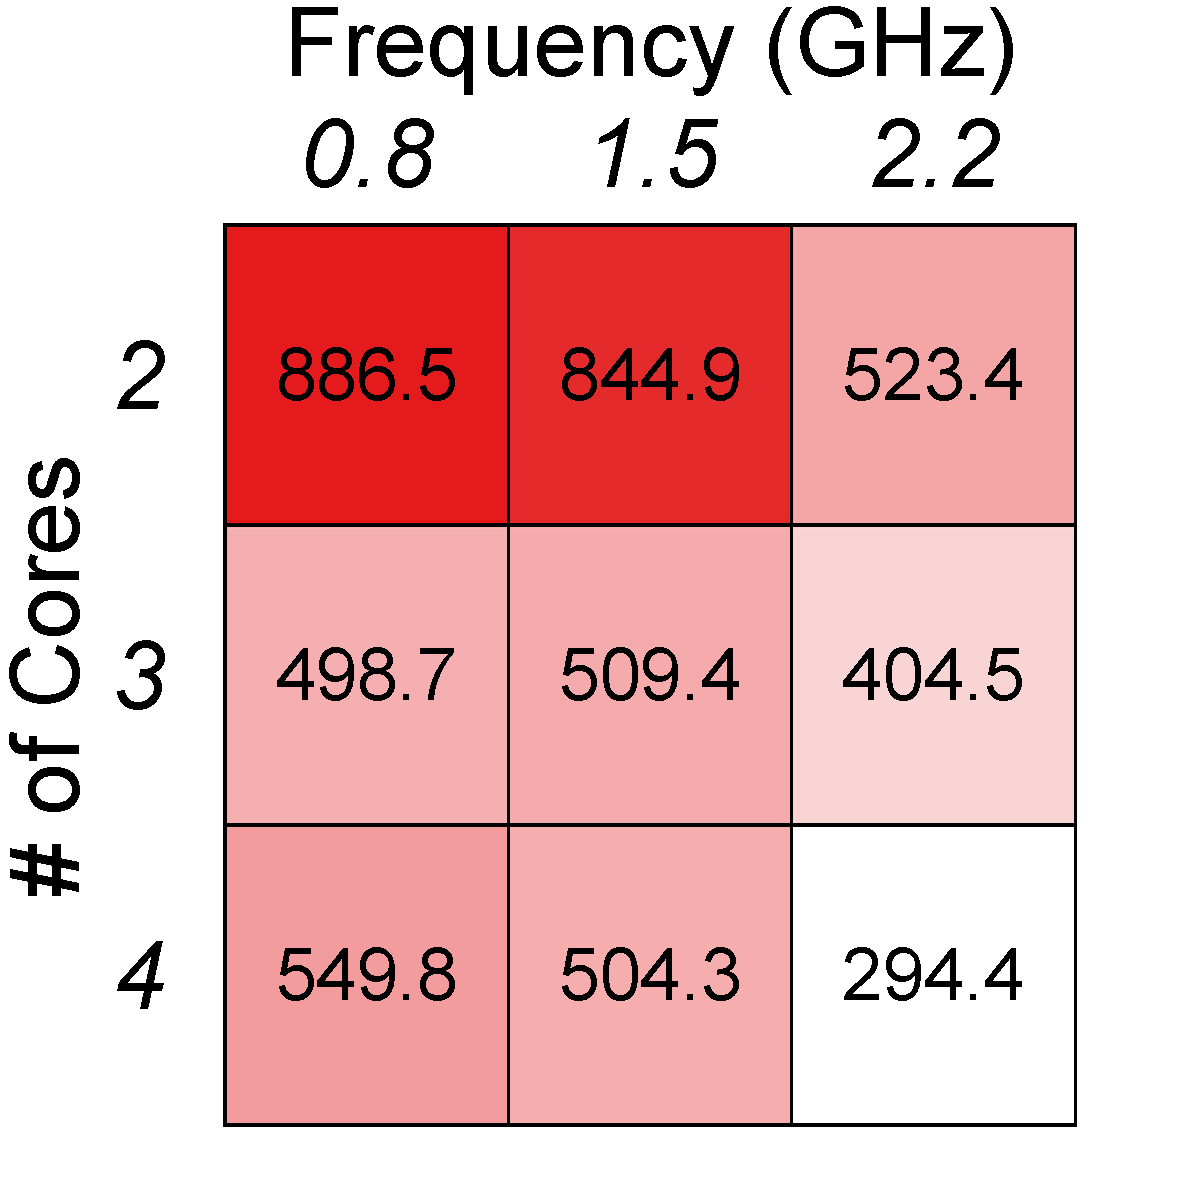
\includegraphics[width=\columnwidth]{figs/SAR_flight_time_operating_point}
    \caption{Mission Time (s)}
    \label{fig:benchmarks:OPA:sar:time}
    \end{subfigure}
    \begin{subfigure}[t!]{.3\columnwidth}
    \centering
    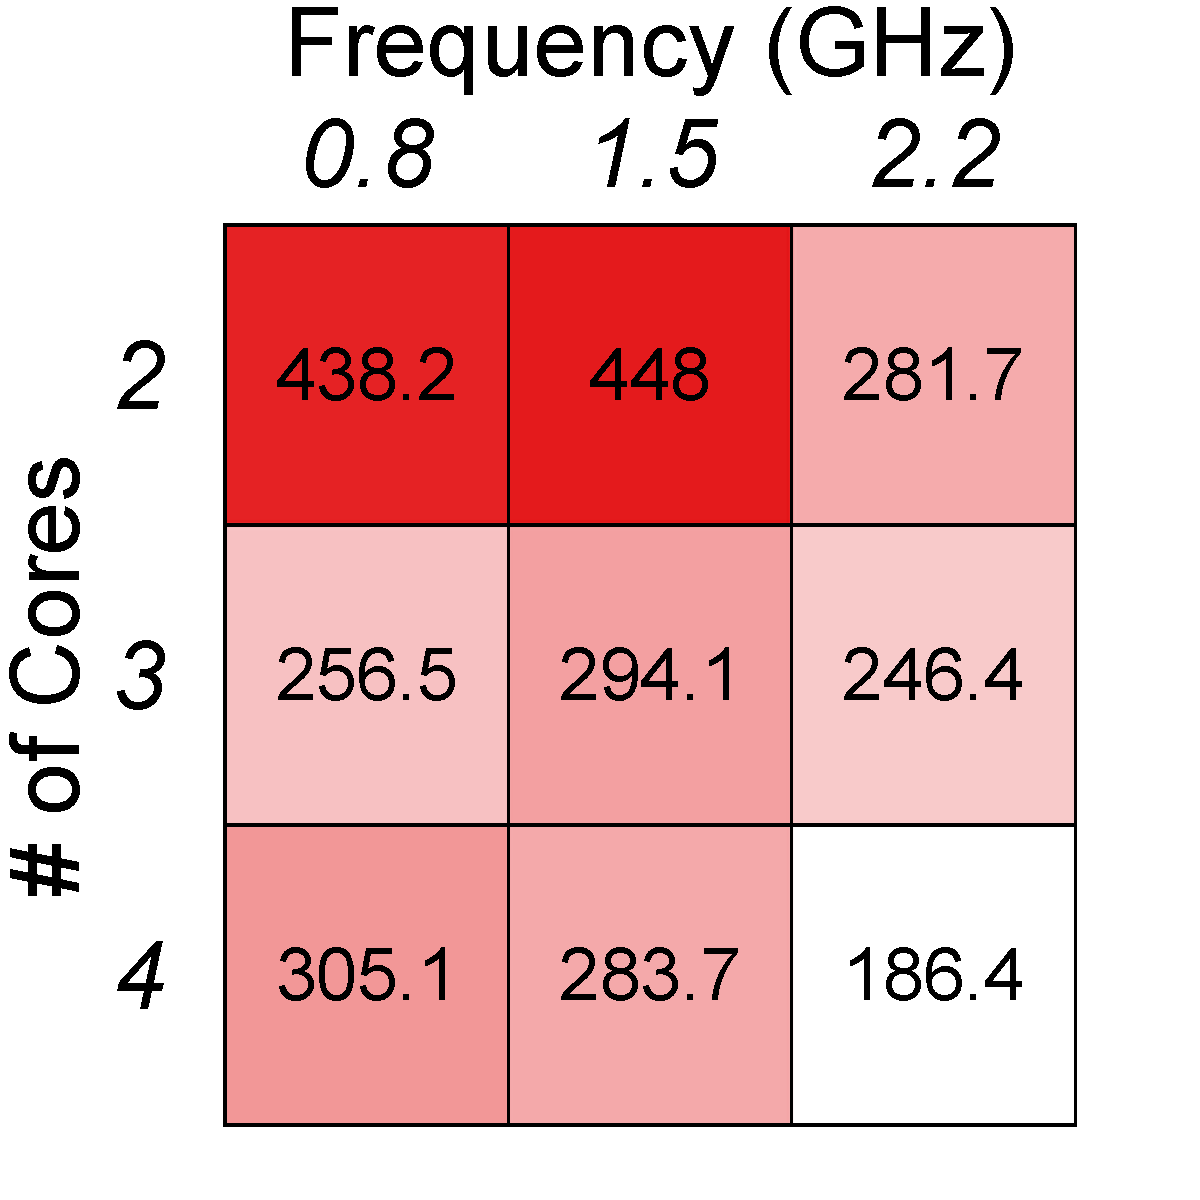
\includegraphics[width=\columnwidth] {figs/SAR_energy_operating_point}
    \caption{Energy (kJ)}
     \label{fig:benchmarks:OPA:sar:energy}
    \end{subfigure}
    \caption{Search and Rescue.}
    \label{fig:benchmarks:OPA:sar}
    \end{figure}
    \begin{figure}[t!]
    \centering
    \begin{subfigure}[t!]{.3\columnwidth}
    \centering
    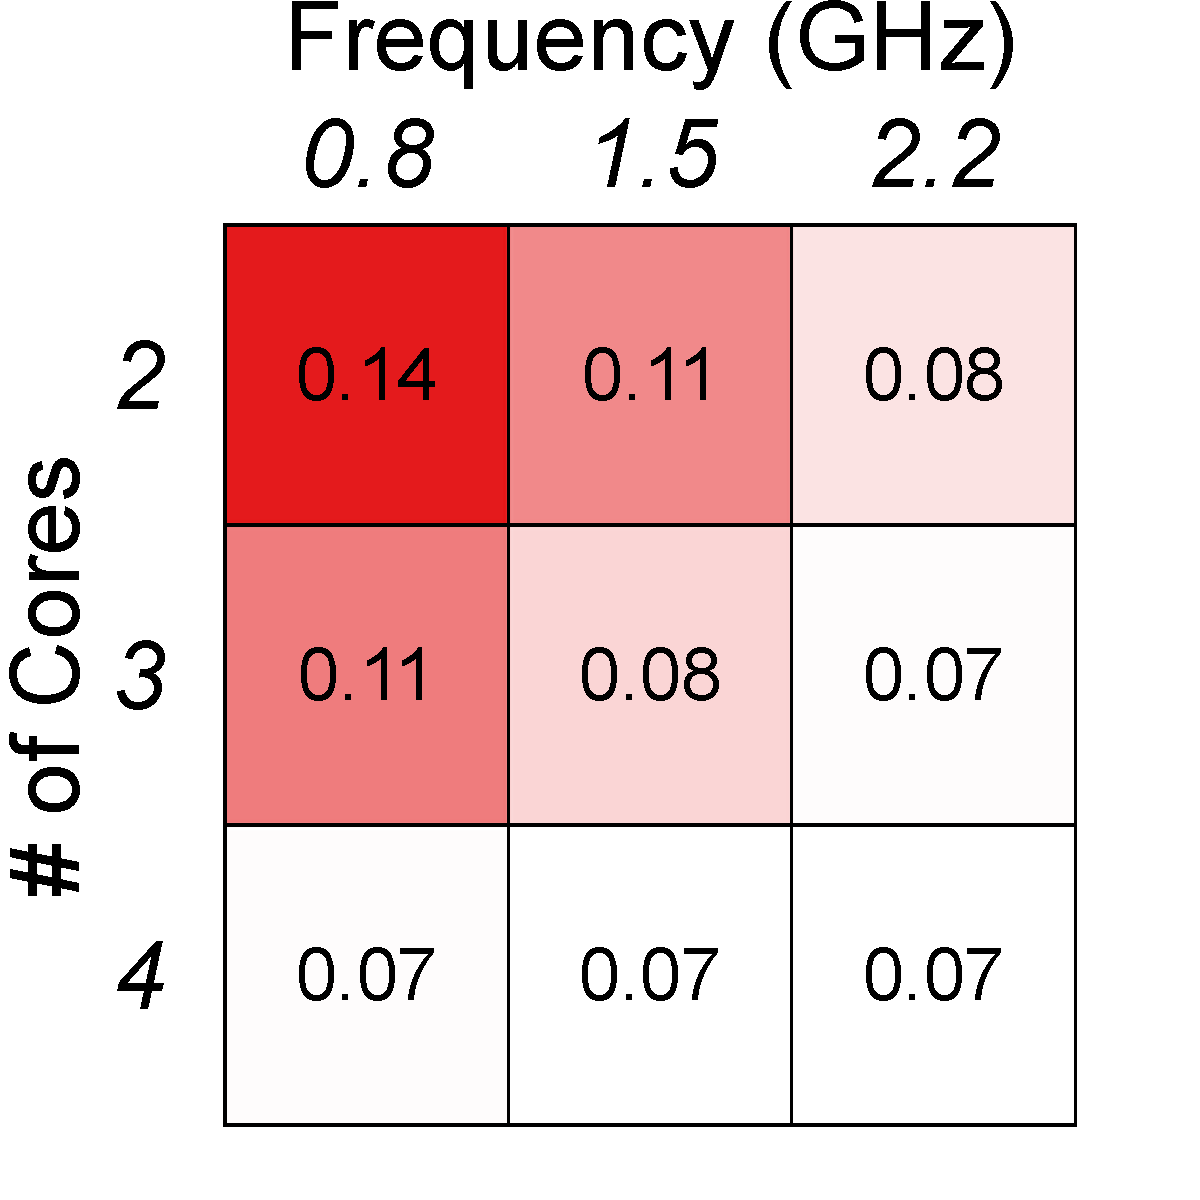
\includegraphics[width=\columnwidth]{figs/aerial_photography_error_operating_point}
    \caption{Error Rate(m/s)}
     \label{fig:benchmarks:OPA:ap:velocity}
    \end{subfigure}
    \begin{subfigure}[t!]{.3\columnwidth}
    \centering
    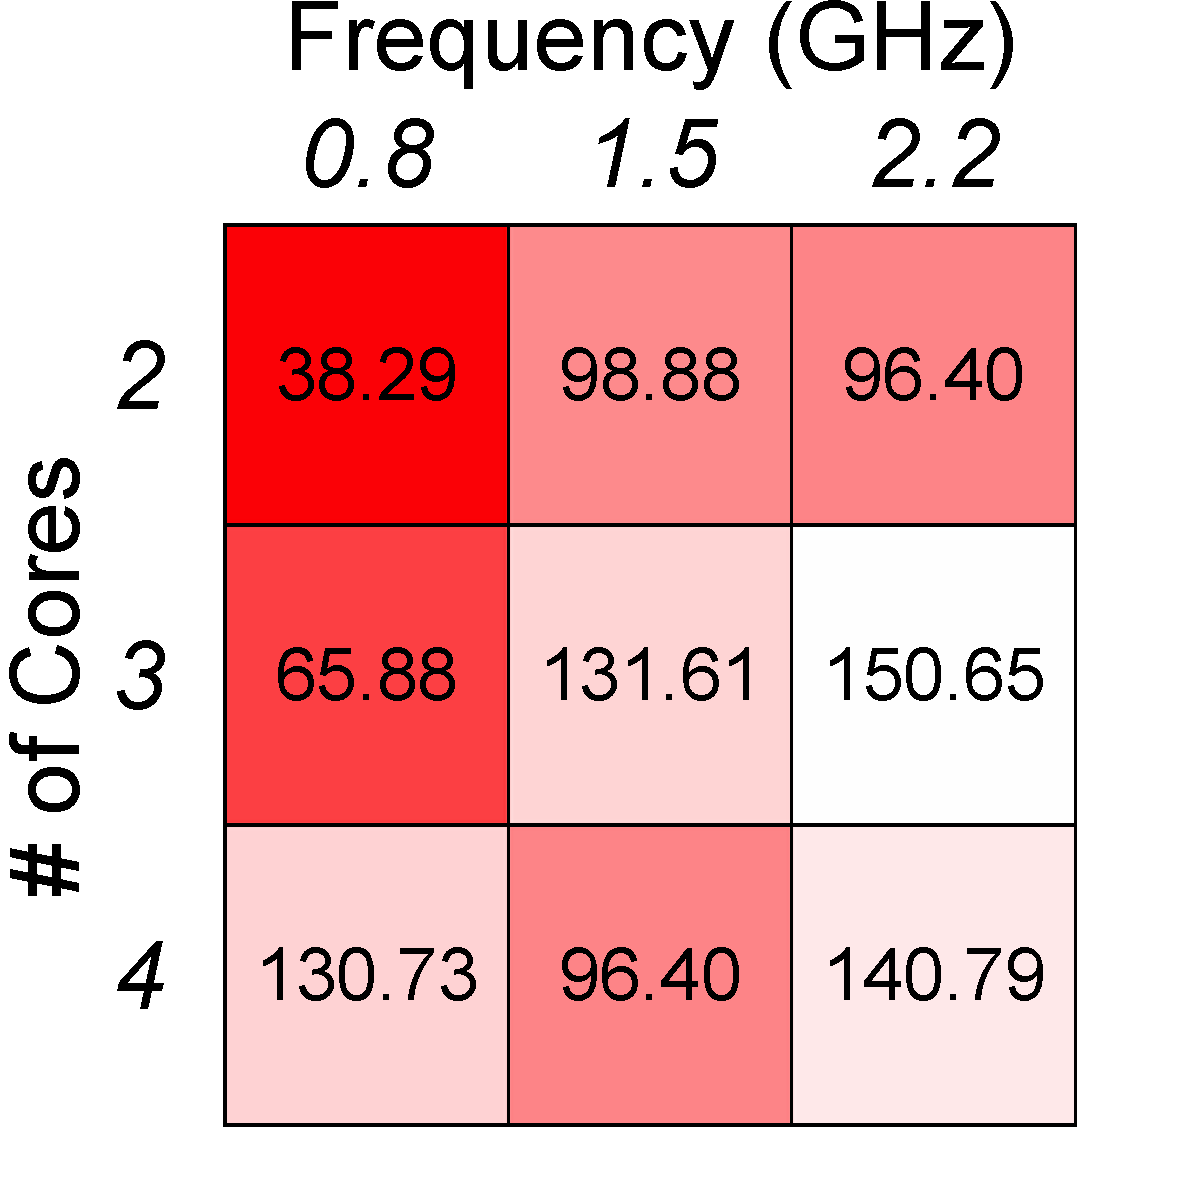
\includegraphics[width=\columnwidth]{figs/aerial_photography_flight_time_operating_point}
    \caption{Mission Time(s)}
    \label{fig:benchmarks:OPA:ap:time}
    \end{subfigure}
    \begin{subfigure}[t!]{.3\columnwidth}
    \centering
    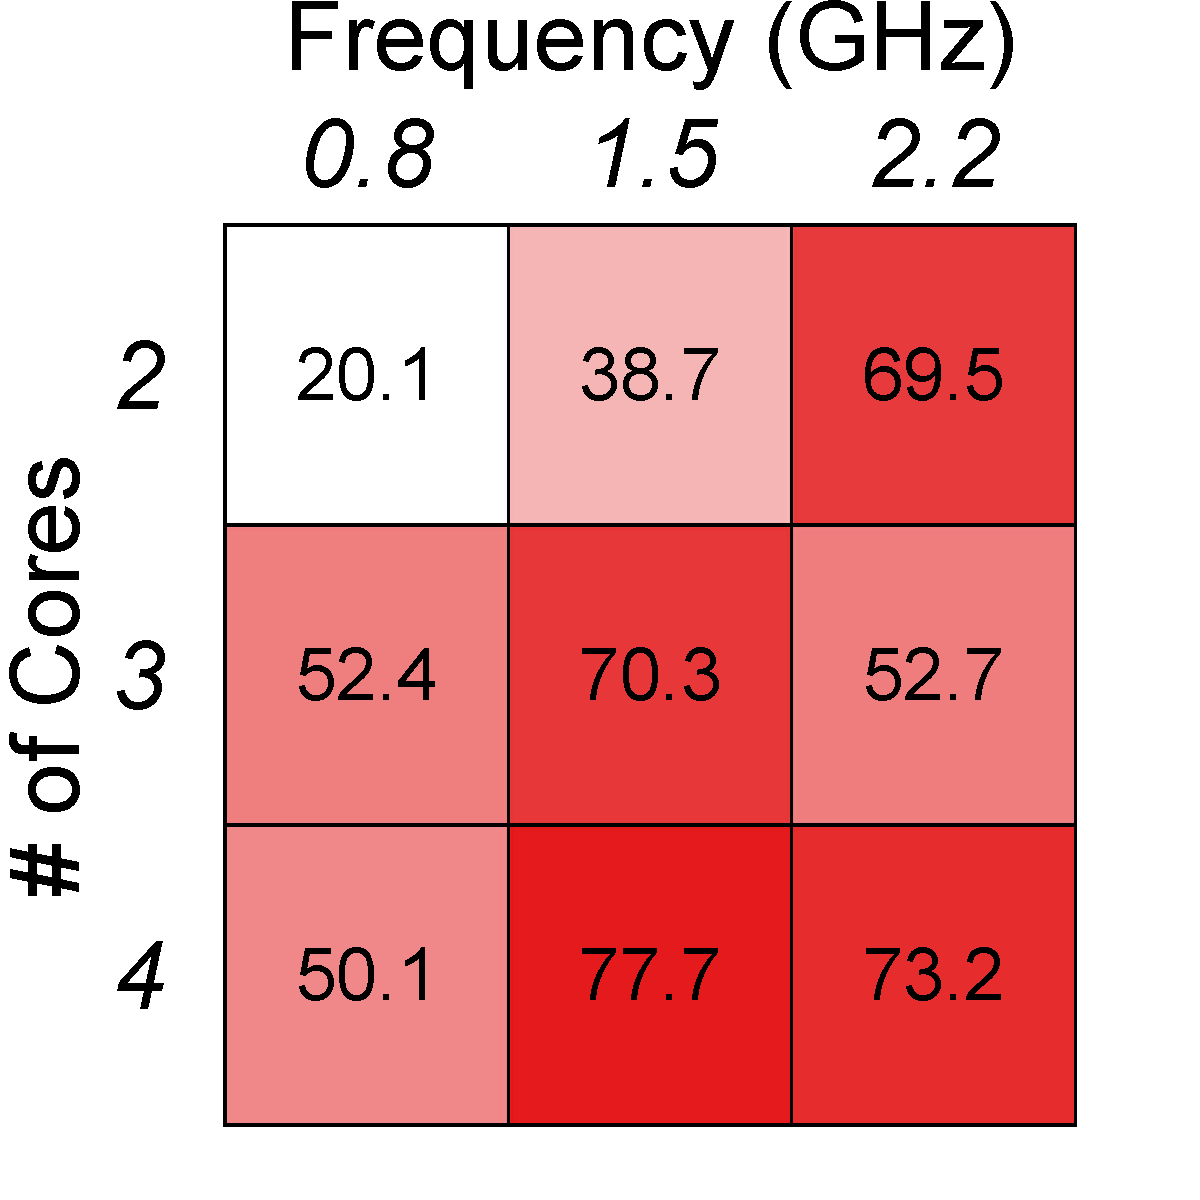
\includegraphics[width=\columnwidth] {figs/aerial_photography_energy_operating_point}
    \caption{Energy (kJ)}
     \label{fig:benchmarks:OPA:ap:energy}
    \end{subfigure}
    \caption{Aerial Photography.}
    \label{fig:benchmarks:OPA:ap}
\end{figure}
}


\paragraph{Mapping:} We observe a reduction of up to 86\% and 83\% for the mission time and energy consumption, respectively, as compute scales with the number of cores and/or frequency values (\Fig{fig:benchmarks:OPA:mapping:velocity}, \Fig{fig:benchmarks:OPA:mapping:time}, and \Fig{fig:benchmarks:OPA:mapping:energy}). The concurrency present in this application (all nodes denoted by circles with a filled arrow connection or none at all in \Fig{fig:benchmarks:data-flow:mapping} run in parallel) justifies the performance boost from core scaling. The sequential bottlenecks, i.e. motion planning and OctoMap generation explains the frequency scaling improvements. We achieve up to 6.3X improvement in motion planning (\Fig{fig:kernel-breakdown}) and that leads to hover time reduction. We achieve a 6X improvement in OctoMap generation and that leads to maximum velocity improvement. The improvements translate to a 5.3X improvement in average velocity. Since mission time is reduced, total energy consumption reduces.


\paragraph{Search and Rescue:} We see a reduction of up to 67\% and 57\% for the mission time and the energy, respectively, as compute scales (\Fig{fig:benchmarks:OPA:sar:velocity}, \Fig{fig:benchmarks:OPA:sar:time}, and \Fig{fig:benchmarks:OPA:sar:energy}). Similar to mapping, more compute allows for the reduction of hover time and an increase in maximum velocity which contribute to the overall reduction in mission time and energy. In addition, a faster object detection kernel prevents the drone from missing sampled frames during any motion. We achieve up to 1.8X, 6.8X, and 6.6X speedup for the object detection, motion planning and OctoMap generation kernels, respectively. In aggregate, these improvements translate to 2.2X improvement in the MAV's average velocity.

\begin{comment}
\begin{figure}[!t]
\centering
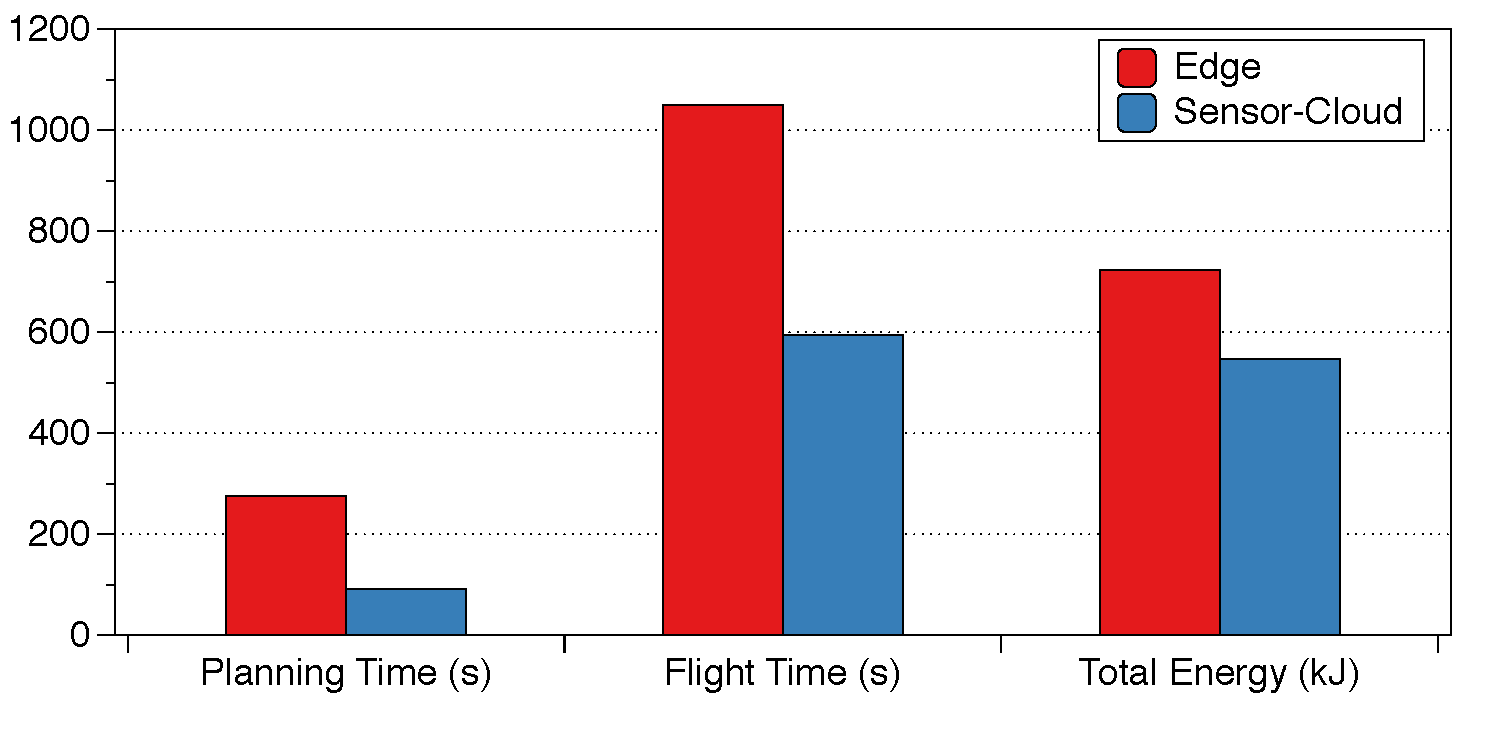
\includegraphics[trim=0 0 0 -25, clip, width=0.9\linewidth]{figs/tx2-desktop}
\vspace{-12pt}
\caption{Comparing a full-on-edge drone versus a full-on-cloud drone. Our system allows part or portion of the MAVBench workloads to be offloaded to the cloud (or another local co-processing agent).}
\label{fig:cloud_edge}
\end{figure}
\end{comment}

\paragraph{Aerial Photography:} We observe an improvement of up to 53\% and 267\% for \emph{error} and mission time, respectively (\Fig{fig:benchmarks:OPA:ap:velocity}, \Fig{fig:benchmarks:OPA:ap:time}, and  \Fig{fig:benchmarks:OPA:ap:energy}). In aerial photography, as compared to other applications, higher mission time is more desirable than a lower mission time. The drone only flies while it can track the person, hence a longer mission time means that the target has been tracked for a longer duration. In addition to maximizing the mission time, error minimization is also desirable for this application. We define error as the distance between the person's bounding box (provided by the detection kernel) center to the image frame center.  Clock and frequency improvements translate to 2.49X and 10X speedup for the detection and tracking kernels and that allows for longer tracking with a lower error. No significant trend is observed in the energy data because energy depends on both the mission time and the velocity, and as opposed to the other applications, there is no need for the drone to minimize its velocity. Instead, it needs to successfully track the person.


\begin{figure*}[!t]
\centering
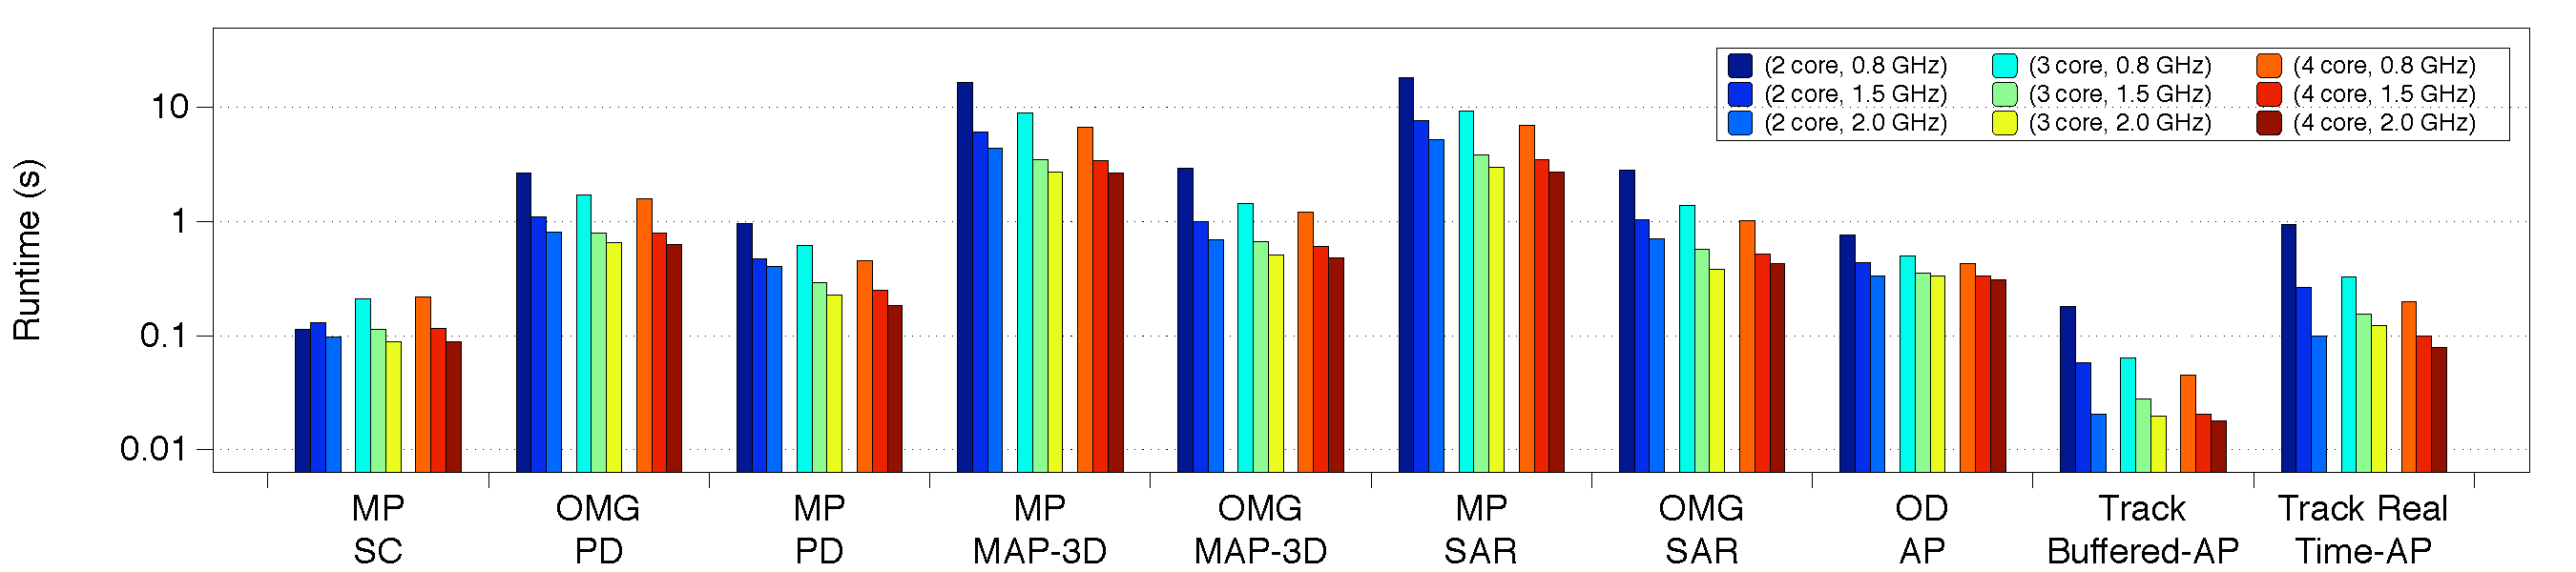
\includegraphics[width=\columnwidth]{figs/kernel-breakdown_2}
\vspace{-18pt}
\caption{Kernel breakdown for MAVBench. The abbreviations are as follows: \emph{OD-}Object detection, \emph{MP-}Motion Planning, \emph{OMG-}OctoMap Generation for kernels and \emph{SC-}Scanning, \emph{PD-}Package Delivery,  \emph{MAP-}3D Mapping, \emph{SAR-}Search and Rescue, and \emph{AP-}Aerial Photography for applications. The $x$-axis lists the kernel-application names and $y$-Axis represents the runtime in seconds. Each bar graph represents one of the configurations used in the hardware. The cores are varied from 2 to 4 and the frequency goes from from 0.8 GHz , 1.5 GHz or 2.2 GHz.}
\label{fig:kernel-breakdown}
\end{figure*}

%\begin{minipage}[!]{0.99\columnwidth}
   
%\end{minipage}


%In the perception stage of this application, a person is detected, and the bounding box associated with the person is tracked. The tracking stage consists of two nodes itself. The first node (buffer then track) buffers the images while detection is running and then track the buffered once the person is detected. The second node (track continuously) tracks the previous bounding box while the new one is calculated. Buffer then track node is necessary, since otherwise, image difference between the image detection sampled and tracking is large enough that increases the false positive tracking. PID node calculates the difference between the targets place and where it should be in the frame and sends small trajectories to the drone. Similar to other applications, these trajectories are followed in the follow trajectory node.

%Compute's effect on this application is on its accuracy and the duration in which drone can follow the target. In other words, faster compute can affect how closely and for how long the target is tracked. 
%\subsection{Understanding the Compute to Endurance Relationship}
%in this section, we demonstrate the relationship between compute on the drone and the drone's mission time (i.e., endurance). We start by showing that looking naively indicates that compute consumes an insignificant amount of power, and that much of the power is spent on keeping the drone afloat using its rotors. Therefore, this leads to a shortsighted conclusion that compute does not play a dominant role in autonomous flight for dron

%\subsection{Micro architectural characterization}
%To understand the reason behind the aforementioned bottlenecks, we provide micro-architectural characterization of them. This will help the designers to design for the future MAV systems while alleviating such bottlenecks. Our analysis show that the bottle necks mainly exists in the perception and the planning stage. Hence, we turn our focus solely to these two stages.  
%
%characterize OctoMap, slam and nbvPlanner. 

\begin{comment}
%\subsubsection{Algorithmic Choices}
%Algorithms at some point will be general enough to cover all the environments, hence we shouldn't 
%be highlighting our algorithmic sensitivity to environment (which in this argument is considered in a flaw)
 
\subsection{explanation of each apps inter kernel interactions}
\textbf{Scanning:} This application involves only a single ROS node. All the code runs on a CPU, with no parallelization. The main computational kernel is the simple path-planning since no collision-checking is involved. This is because the \textit{Scanning} benchmark is meant for outdoors environments, high aboveground where obstacles are not to be found. Because the benchmark is meant for outdoors environments, localization is accomplished through the use of GPS sensors, which incur negligible computational overhead.

\textbf{Aerial Photography}
This application involves three ROS nodes running concurrently. One node is responsible for running object detection algorithms to locate the human target. However, object detection is normally a very computationally-intensive task that can take up to several seconds to complete. Therefore, another node runs much faster tracking algorithms such as KCF which estimate the position of the target in the interval between completions of the object detection algorithm. Another node controls the motion of the MAV based on the position of the target. All nodes run on the CPU except for the object detection node which runs on a GPU.

\textbf{Package delivery:}
This application involves 4 ROS nodes, which all run on CPU cores. One node plans collision-free trajectories using the path-planning algorithms described in the previous section. Another node waits for paths to be planned and then controls the motion of the MAV to follow them. However, as the MAV follows these trajectories, it may uncover new obstacles in its environment that had been out of range of its sensors when the path was initially planned. Therefore, an additional node must constantly run to check whether any newly uncovered obstacle causes a collision upon the planned trajectory, so that the path can be re-planned if necessary. Finally one final node must provide localization capabilities, either through GPS or SLAM, to enable the MAV to follow its planned trajectory accurately.

\textbf{Mapping}
This application involves 3 ROS nodes which all run on CPU cores. One node samples its environment and finds points on the boundary of previously explored space where the MAV can be expected to maximize the amount of unknown space that it uncovers. Once these points are found, the node then plans a path towards them along an RRT tree. A second node controls the motion of the MAV, following the trajectories generated by the first node. Finally, a third node must provide localization, such as through SLAM. This localization must be accurate, because the MAV updates its internal map based upon the position it believes it is in. If the MAV relies upon an inaccurate SLAM algorithm, the map it generates may not be completely accurate.


\textbf{Exploration:}
Computationally, this application includes the same nodes as the \textit{Exploration} benchmark, as well as another node that constantly runs object detection algorithms to search for human victims as it explores unknown environments. The object detection node here runs on a GPU. The object detection algorithm must run fast, in order to allow the MAV to sweep a large area quickly, but they must also be highly accurate, to prevent the MAV from missing a victim due to a false negative.


\label{sec:characterization}
 possibly the bottlenecks, and a table with kernel times and their distribution.
 
 possibly the requirements compute wise and which platforms are suitable for them (refer back to the HIL and how we can conduct these conclusive studies)

\subsection{Environment and it's effects}
indoor/outdoor,
obstacle density, dynamic obstacle speed
\subsection{}

\end{comment}

 

%\section{Compute-driven, Flight-Efficiency Optimization: A Case Study}
 
\label{sec:energy-case-study}
\section{Case Studies}
\label{sec:case-study}


We show how our closed-loop simulation, along with our open-source benchmark suite, can enable (1) performance, (2) energy and (3) reliability studies, both at the architecture and the holistic system-level. MAVBench simulation setup allows for inspection of intra-system, as well as system and environment interactions. Studying the intra-system interactions opens new avenues for hardware and software co-design, which we demonstrate in the form of onboard/edge-only compute versus offloading the compute to the unconstrained cloud. Studying the system and environment interactions can unlock new opportunities for trade-offs in computational complexity for energy efficiency, which we demonstrate using software-guided, hardware-assisted OctoMap resolution optimizations.

\subsection{A Performance Case Study}


As opposed to the study in Section~\ref{sec:char} where we emulated a fully-on-edge drone (i.e., a drone which all of its computation is done on the drone itself), we examine a cloud/edge drone where the computation is distributed across the edge and the cloud. We compare a fully-on-edge drone equipped with a TX2 versus a fully-in-cloud drone with a powerful cloud support. The ``cloud'' computational horsepower is composed of an Intel i7 4740 @ 4GHz with 32 GB of RAM and a GeForce GTX 1080. For network connectivity we utilize a 1Gbp/s LAN, which mimics a future 5G network~\cite{agyapong2014design, gupta2015survey}.

\begin{figure}[b!]
\centering
    \begin{subfigure}{.608\columnwidth}
    \centering
    \includegraphics[trim=5 0 20 0, clip, width=\columnwidth]{figs/tx2-desktop_performance}
    \caption{Performance.}
    \label{Perforamnce}
    \end{subfigure}
    \hfill
    \begin{subfigure}{.365\columnwidth}
    \centering
    \includegraphics[trim=5 10 0 0, clip, width=\columnwidth]{figs/tx2-desktop_energy}
    \caption{Energy.}
    \label{fig:drone-power-time-series}
    \end{subfigure}
\caption{Comparing a full-on-edge drone versus a full-on-cloud drone. Our system allows part or portion of the MAVBench workloads to be offloaded to the cloud (or another local co-processing agent).}
\label{fig:cloud_edge}
\end{figure}

We target the planning stage of the PPC pipeline and focus on the 3D Mapping as the application of choice to offload. As we show in \Fig{fig:cloud_edge}, a drone that can enjoy the cloud's extra compute power sees a 3X speed up in planning time. This improves the drone's average velocity due to hover time reduction, and hence reduces the drone's overall mission time by as much as 50\%, effectively doubling its endurance.

\begin{figure*}[!t]
\vspace{-12pt}
    \centering
    \begin{subfigure}[t]{.24\linewidth}
        \centering
        \includegraphics[height=1.4in]{figs/garage_sim}%
         \vspace{-20pt}
        \caption{Environment's map.}%
        \label{fig:garage_sim}
    \end{subfigure}
    \hfill
    \begin{subfigure}[t]{.24\linewidth}
        \centering
        \includegraphics[height=1.4in]{figs/garage_rviz__15}%
         \vspace{-20pt}
        \caption{Resolution of 0.15 \emph{(m)}.}%
        \label{fig:rviz__15}
    \end{subfigure}
    \hfill
     \begin{subfigure}[t]{.24\linewidth}
        \centering
        \includegraphics[height=1.4in]{figs/garage_rviz__5}%
      \vspace{-20pt}
     \caption{Resolution of 0.5 \emph{(m)}.}%
        \label{fig:game:rviz__5}
    \end{subfigure}
       \hfill
   \begin{subfigure}[t]{.24\linewidth}
        \centering
        \includegraphics[height=1.4in]{figs/garage_rviz_1}%
        \vspace{-20pt}
        \caption{Resolution of 0.80 \emph{(m)}.}%
        \label{fig:game:rviz_1}
    \end{subfigure}
    \hfill\\[15pt]
   \vspace{-25pt}
   \caption{For the environment in \emph{(a)}, OctoMap's resolution impact on the drone's perception of its environment is shown in \emph{(b)}, \emph{(c)}, \emph{(d)}.}
    \label{fig:octomap_perception}
\end{figure*}

\begin{figure}[t]
\vspace{0pt}
\centering
\includegraphics[trim=0 0 30 0, clip, width=\columnwidth]
%\includegraphics[trim=0 0 0 0, clip, width=1.0
%\linewidth]%
{figs/octomap_resolution_case_study}
%{figs/octomap_resolution_with_boxes}
%\vspace{-50pt}
\vspace{-23pt}
\caption{Reduction in OctoMap resolution (accuracy) can be traded off with processing time. Increasing the $x$-axis means larger voxels to represent the space more coarsely (less accurately). A 6.5X reduction in resolution results in a 4.5X improvement in processing time.}
%\vspace{15pt}
\label{fig:octrest}
\end{figure}


\subsection{An Energy Case Study} 

Focusing on energy efficiency, we conduct a kernel/environment sensitivity analysis using the OctoMap node~\cite{octomap}, which is a major bottleneck in three of our end to end applications, namely package delivery, 3D mapping and search and rescue. OctoMap is used for the modeling of various environments without prior assumptions. The map of the environment is maintained in an efficient tree-like data structure while keeping track of the free, occupied and unknown areas. Both planning and collision avoidance kernels use OctoMap to make safe flight possible, via costly compute cycles, by only allowing navigation through free space. Due to its implementation efficiency, OctoMap is widely adopted in the robotics community. Its broad adoption and impact in two out of three stages (Perception and Planning) makes this kernel highly general and important for optimization.

The size of the voxels in OctoMap, i.e. the map's resolution, introduces accuracy versus flight-time/energy trade-off. By lowering the resolution, i.e. increasing \emph{voxel} sizes, obstacle boundaries get inflated, hence the drone's perception of the environment and the objects within it becomes inaccurate. We illustrate the impact of OctoMap resolution on the drone's perception using \Fig{fig:octomap_perception}. \Fig{fig:garage_sim} {shows the environment and  Figures~\ref{fig:rviz__15}, \ref{fig:game:rviz__5}, \ref{fig:game:rviz_1} show the drone's perception of the environment as a function of OctoMap resolution. When the resolution is lowered, the voxels size increases to the point that the drone fails to recognize the openings as possible passageways to plan through (Figure~\ref{fig:game:rviz_1}). This results in mission time inefficiency and failures depending on the environment.

To examine the accuracy versus performance trade off, we measured OctoMap kernel's processing time (running in isolation) while varying its resolution knob. \Fig{fig:octrest} shows that as planning resolution increases (i.e., voxels are larger so space is represented more coarsely and hence less accurately), performance improves dramatically because less compute is needed. Going from one extreme to another, when planning resolution goes from less than 0.2~m to 1.0~m ($x$-axis), OctoMap's processing time (or update rate) goes from more than 0.4~seconds to less than 0.1~seconds ($y$-axis). In other words, a 6.5X reduction in accuracy results in a 4.5X improvement in processing time.


\begin{figure}[t]
%\vspace{-5pt}
\centering
\includegraphics[trim=0 0 0 0, clip, width=\columnwidth]
%\includegraphics[trim=0 0 -5 -25, clip, width=0.9\linewidth]
%\includegraphics[height=5cm,keepaspectratio]
%\includegraphics[width=\columnwidth]%
%\includegraphics[trim={0 0 0 5cm}, clip, width=\columnwidth]%
{figs/energy-case-study}
\vspace{-23pt}
%\vspace{-15pt}
\caption{Switching between OctoMap resolutions dynamically leads to successfully finishing the mission compared to 0.80~m. It also leads to battery life improvement compared to 0.15~m. The $y$-axis in the top graph is the battery left on the drone upon mission completion.}
%\vspace{15pt}
\label{fig:dual-res}
\end{figure}



\begin{comment}
\begin{table}[t]
\vspace*{20pt}
\centering
\vspace{-14pt}
\caption{Switching between OctoMap resolutions dynamically leads to mission success compared to 0.8~m, and compared to 0.15~m we consume less energy and thus retain more battery.}
\label{tbl:octopt}
\resizebox{1.0\columnwidth}{!}{
\begin{tabular}{l|l|l|l|}
\cline{2-4}
\textbf{Resolution {(m)}}       & \textbf{Mission Status} & \textbf{Battery  (\%)} \\ \hline
\multicolumn{1}{|l|}{\multirow{3}{*}{\textbf{Package Delivery}}} & \textit{0.8}              & \cellcolor{red!25}Fail                    &   0           \\ \cline{2-4} 
\multicolumn{1}{|l|}{}                                           & \textit{0.15}             & Pass                    &    81.00          \\ \cline{2-4} 
\multicolumn{1}{|l|}{}                                           & \textit{Chameleon (0.8, 0.15)} & Pass                    &   \cellcolor{green!25}86.00           \\ \hline
\multicolumn{1}{|l|}{\multirow{3}{*}{\textbf{Mapping}}}          & \textit{0.8}              & \cellcolor{red!25}Fail                    & 0           \\ \cline{2-4} 
\multicolumn{1}{|l|}{}                                           & \textit{0.15}             & Pass                    & 39.03        \\ \cline{2-4} 
\multicolumn{1}{|l|}{}                                           & \textit{Chameleon (0.8, 0.15)} & Pass                    & \cellcolor{green!25}53.83        \\ \hline
\multicolumn{1}{|l|}{\multirow{3}{*}{\textbf{Search and Rescue}}}              & \textit{0.8}              & \cellcolor{red!25}Fail                    & 0         \\ \cline{2-4} 
\multicolumn{1}{|l|}{}                                           & \textit{0.15}             & Pass                    & 24.21        \\ \cline{2-4} 
\multicolumn{1}{|l|}{}                                           & \textit{Chameleon (0.8, 0.15)} & Pass                    & \cellcolor{green!25}57.87        \\ \hline
\end{tabular}
}
\end{table}
\end{comment}


Certain aspects like obstacle density in the environment determine the ``ideal'' OctoMap resolution. In low-density environments, where the drone has many obstacle-free paths to take, a low resolution can suffice. In dense environments, low resolutions can deprive the drone of viable obstacle-free paths because the drone perceives the obstacles to be larger than they are in the real world, and so plans to avoid them. Since the drone's environment constantly changes, a dynamic approach where a runtime sets the resolution is ideally desirable.

We study two environments during the mission, namely outdoors (low obstacle density) and indoors (high obstacle density). \Fig{fig:dual-res} shows the result of two static (predetermined) resolutions, 0.15~m and 0.80~m, and our dynamic approach that multiplexes between the two appropriately.\footnote{Resolutions are based on the environment like the door width size. A 0.15~m resolution is chosen to ensure that the drone (diagonal width of 0.65~m) considers an average door (width of 0.82~m) as an opening for planning.} The dynamic approach allows improvement of battery consumption by up to 1.8X. 
%life for up to 43\%. To compute this improvement, we calculate the difference between the dynamic and static battery consumption and divide it by the static value. For example, for SAR, $\frac{(76\%- 43\%)}{76\%}$ leads to a 43\% improvement. 
Intuitively, as compute reduces, OctoMap bottleneck eases, and therefore the drone completes its mission faster. The figure also highlights another interesting relationship that statically choosing the 0.80~m resolution to optimize for compute (only) causes the drone to fail its mission since it is unable to plan paths through narrow openings in the indoor environments. Instead, by switching between the two resolutions according to the environment's obstacle density, the dynamic approach is able to balance OctoMap computation with mission feasibility and energy, holistically. Therefore, in all cases, the dynamic approach uses less energy and retains more battery life at mission end time.


% Please add the following required packages to your document preamble:
% \usepackage{multirow}


\subsection{A Reliability Case Study}

Reliability is an especially important topic in the context of autonomous vehicles~\cite{reli-1, reli-2, reli-3, reli-4}. Traditionally, it is common to study the susceptibility of execution to errors that manifest in programs and the architecture. In autonomous vehicles, errors or ``noise'' in the data can arise from sensor inputs. 

We investigate the impact of sensor noise on the performance of our package delivery application, specifically its perception stage. The data is summarized in Table~\ref{tbl:noise-data}. We inject Gaussian noise with a range of standard deviations (0 to 1.5~m) into the depth readings of the drone's RGBD camera. The sensory noise distorts the drone's perception of the obstacles in its environment, and we found such noise \emph{inflates} obstacles, making them appear larger than they are in reality. This causes the drone to re-plan its trajectories more often, as it assumes that its planned path will collide into objects that are actually further away than they seem. The more the drone re-plans its paths, the longer it takes to reach its destination, which increases it mission time by up to 90\%. It is also important to note that when noise values reach greater than a certain value, it causes the drone to fail in its mission altogether, e.g. noise with the standard deviation of 1.5~m results the drone to fail reaching its delivery destination in 10\% of its total runs. 

In addition to injecting noise in the sensor subsystem, we can also inject errors directly into the compute subsystem to ``simulate'' soft errors and transient bit flips in logic. Such a capability can be used to conduct vulnerability analysis~\cite{mukherjee2005soft}.

%\section{Context-Sensitive Optimization}
\label{sec:optimization}

As was shown in the previous section, the OctoMap generation node plays a crucial role in performance and energy consumption of drones.
This node is used for modeling of various environment without prior assumptions. In order to do so, the map of the environment is maintained in an efficient tree-like data structure while keeping track of free, occupied and unknown areas. Both planning and collision avoidance kernels utilize this data structure to make safe flights possible by only allowing the drone to navigate through free spaces.  

size of the voxels, i.e. the map's resolution, trades off accuracy and flight-time/energy. By lowering the resolution, i.e. increasing voxel sizes, obstacle boundaries get inflated, hence drones perception of the environment and the objects within it becomes inaccurate. However, doing so improves the performance of the OctoMap generation node and eventually leads to a faster flight time.  As figure blah shows blahx speed up in the update rate of OctoMap is achievable for a sacrifice of blahx in resolution. 

To study the effect of this knob on our applications we conducted a study where the drone will conduct some part of its mission in less dense environment such as outdoors and part of it in more dense environment such as indoors. We 



the  the flight time and the energy consumption of the drone. This node is responsible for providing the 
\section{Related Work}
\label{sec:related}

There is prior work that focuses on building simulators and benchmark suites to aid the development of autonomous MAVs. We address some shortcomings of previous approaches by providing a more integrated, end-to-end solution.

\paragraph{Simulators} Simulators are essential to the study of aerial and robotic agents. Our simulation platform is built upon Microsoft's AirSim~\cite{Airsim_paper}, a UAV simulator that uses the Unreal Game Engine to provide accurate physics models and photo-realistic environments. MAVBench uses the AirSim core and extends it with performance, power and battery models that are suited for architectural research, as well as with a gimbal, and dynamic and static obstacle creation capabilities that are not inherently part of AirSim. Another very popular simulator used in the robotics community for MAVs is Gazebo~\cite{gazebo}. However, Gazebo simulations lack photo-realism, while our work, with the help of AirSim and the Unreal Game Engine, enables more accurate visual modeling.

There are also numerous simulators widely used in industry and academia for studying autonomous agents such as ~\cite{boss-cmu,talos-mit,odin-vtech,uber-simulator, uav_benchmark_simulator}. However, they either do not provide MAV models or does not consider the architectural insights.

%For instance, one such simulator, CARLA~\cite{carla} also uses the Unreal engine for photo-realistic representations of the environment. However, CARLA lacks models for MAVs, rotor dynamics and their interaction with the environment. For MAVs, there has been prior work~\cite{uav_benchmark_simulator} using simulators built on the Unreal game engine. However unlike ours, their work mainly focuses on object tracking and does not go into the evaluation of the hardware platform and system architecture. 

A recent work FlightGoggles~\cite{flight-goggles}, creates virtual reality environments for drones using the images streamed from the Unity3D game engine. However, for maximum realism, FlightGoggles requires a fully functioning drone that must fly during tests, with its sensory data being streamed in from the game engine. MAVBench, on the other hand, does not have this constraint. Our users may provide real processors for hardware-in-the-loop simulation, but they are not required to fly the MAVs physically in the real world.

\paragraph{Benchmarks} Most robot benchmark suites target individual computational kernels, such as odometry or motion-planning, rather than characterizing end-to-end applications composed of many different kernels. For example SLAMBench~\cite{slambench} and CommonRoad~\cite{common-road} solely focus on the perception and the planning stage respectively. However, our benchmarks allows for holistic studies by providing end-to-end applications. 
%For example, there are numerous robotic vision datasets, such as KITTI~\cite{kitti}, and the EuRoC~\cite{euroc} MAV dataset, but these focus exclusively on the perception stage of a robot's computational pipeline. Others such as SLAMBench~\cite{slambench} and CommonRoad~\cite{common-road} lack 
%a software framework that characterizes the accuracy, performance, and energy consumption of RGB-D SLAM algorithms, and goes far deeper into its analysis of the SLAM computational kernel than we do in MAVBench. However, these tools do not provide insights into how SLAM interacts with other kernels in an end-to-end application. CommonRoad~\cite{common-road} is another benchmarking tool that characterizes motion-planning algorithms for autonomous cars, but computational kernels such as mapping and localization, that are necessary for an end-to-end characterization, are outside its scope.

\renewcommand*{\arraystretch}{1.2}
\begin{table}[t!]
\vspace{10pt}
\caption{Impact of introducing depth image noise into the RGBD camera system on the drone's performance. Introducing noise into the drone's visual subsystem results in more frequent (re-)planning, which increases mission time and can also result in mission failures.}
\label{tbl:noise-data}
\resizebox{1.0\columnwidth}{!}{
\begin{tabular}{|c|c|c|c|}
\hline
\textbf{Noise Std {(m)}} & \textbf{Failure Rate {(\%)}} & \textbf{Number of Re-plans} & \textbf{Mission Time {(s)}} \\ \hline
\rowcolor{red!10}0.0             & 0                 & 2                  & 72               \\ \hline
\rowcolor{red!25}0.5            & 0                 & 3                  & 82               \\ \hline
\rowcolor{red!50}1.0             & 0                 & 4                  & 95               \\ \hline
\rowcolor{red!100}1.5           & 10                & 8                  & 137              \\ \hline
\end{tabular}
}
\end{table}
\renewcommand*{\arraystretch}{1}
\section{Conclusion}
\label{sec:conclusion}

% MAVs have seen an outburst of attention recently, specifically in the area with a demand for autonomy. Despite their ample use cases, e.g. package delivery, and high constraints, e.g. power and performance, these systems have seen a modest examination from the software and hardware architects. 

MAVBench is a tool including a closed-loop simulation platform and a benchmark suite to probe and understand the intra-system (application data flow) and inter-system (system and environment) interactions of MAVs. This enables us to pinpoint bottlenecks and identify opportunities for hardware and software co-design and optimization. Using our setup and benchmark suite, we uncover a hidden compute to total system energy relationship where faster computers can allow drones to finish missions quickly, and hence save energy. This is because most of the drone's energy is consumed by the rotors, hence, faster compute can cut down on mission time (by increasing the max velocity and reducing the hovering time) and energy accordingly. Our insight allows us to improve MAV's battery consumption by up to 1.8X
%life by up to 43\% 
for our OctoMap case study. 

\section*{Acknowledgements}

This material is based upon work supported by the NSF under Grant No. 1528045 and funding from Intel and Google.


\begin{comment}
On large drones, power goes mainly to motors, no matter how performant a processor is used. On smaller drones, the power consumed by processors becomes much more significant.

Faster computers can allow drones to finish missions faster, saving energy.

Such-and-such applications perform best with computers with such-and-such architectures. For example, such-and-such applications require faster parallel computers, while other applications depend upon fast serial performance.

We introduce a benchmark suite that can be used to test drone performance.
\end{comment}
%%DIF < \section{Compute-driven, Flight-Efficiency Optimization: A Case Study}
\section{\DIFaddbegin \DIFadd{Compute-driven, Flight-Efficiency Optimization: A }\DIFaddend Case \DIFdelbegin \DIFdel{Studies}\DIFdelend \DIFaddbegin \DIFadd{Study}\DIFaddend }
\label{sec:case-study}

Our closed-loop simulation platform, together with our plug and play benchmarks, enables a holistic inspection of intra-system and system/environment interactions. Studying of the former open doors for hardware/software co-design studies. Such studies starts with the profiling and sensitivity analysis as exemplified in the previous section. The latter enables environment focused considerations and designs such \DIFdelbegin \DIFdel{as reliability studies%DIF < , i.e. the effect of various localization kernels and collision avoidance algorithms on the system. 
}\DIFdelend \DIFaddbegin \DIFadd{reliability studies, i.e. the effect of various localization kernels and collision avoidance algorithms on the system. }\DIFaddend In this section \DIFdelbegin \DIFdel{, we conduct performance, energy and reliability case studies  highlighting the insights architects can take advantage of by using our platform.   
}%DIFDELCMD < \red{\subsection{Sensor-cloud: A Performance Case-Study}
%DIFDELCMD < As opposed to the studies provided in the previous section where our setup emulated a fully-on-edge drone (i.e. a drone which all of its computation is done on the drone itself), our setup can further examine a cloud/edge drone where the computation is distributed across the edge and the cloud. To examine the impact of cloud computing for MAVs, we compare a fully-on-edge drone equipped with a TX2 versus a fully-in-cloud drone with only a minimal computer on board (i.e. a flight controller) but a powerful cloud support (mention the x86 platform we used). This case study targets Mapping as the application of choice. As can be seen in Fig.\ref{fig:edge_cloud}, a drone that can enjoy the cloud's extra compute power sees a 3X speed up in planning time. This improves the average velocity of the drone due to the reduction in hover time and hence reduces the overall mission time almost to half.
%DIFDELCMD < }
%DIFDELCMD < \begin{figure}[t!]
%DIFDELCMD < \centering
%DIFDELCMD < \includegraphics[trim=0 0 0 -25, clip, width=0.9\linewidth]{figs/tx2-desktop}
%DIFDELCMD < %%%
%DIFDELCMD < \caption{%
{%DIFAUXCMD
\DIFdelFL{Comparing a full-on-edge drone vs a full-on-cloud drone.}}
%DIFAUXCMD
%DIFDELCMD < \label{fig:cloud_edge}
%DIFDELCMD < \end{figure}
%DIFDELCMD < %%%
\subsection{\DIFdel{Environment Aware Design: An Energy Case-Study}}  
%DIFAUXCMD
\addtocounter{subsection}{-1}%DIFAUXCMD
\DIFdelend \DIFaddbegin \DIFadd{we consider an example of the latter.   
}

\DIFaddend We conduct a kernel/environment sensitivity analysis using the OctoMap node~\cite{octomap}, which is a major bottleneck in \DIFdelbegin \DIFdel{3 of our end to  applications, namely package package delivery, mapping and search and rescue}\DIFdelend \DIFaddbegin \DIFadd{our benchmark suite}\DIFaddend . OctoMap is used for modeling of various environments without prior assumptions. In order to do so, the map of the environment is maintained in an efficient tree-like data structure while keeping track of the free, occupied and unknown areas. Both planning and collision avoidance kernels utilize this data structure to make safe flights possible by only allowing the drone to navigate through free spaces.  

\DIFdelbegin %DIFDELCMD < \begin{figure}[b]
%DIFDELCMD < \centering
%DIFDELCMD < \includegraphics[trim=0 0 0 -25, clip, width=\columnwidth]{figs/octomap_resolution_with_boxes}
%DIFDELCMD < %%%
%DIF < \vspace{-30pt}
%DIFDELCMD < \caption{%
{%DIFAUXCMD
\DIFdelFL{OctoMap accuracy (resolution) versus performance.}}
%DIFAUXCMD
%DIFDELCMD < \label{fig:octrest}
%DIFDELCMD < \end{figure}
%DIFDELCMD < 

%DIFDELCMD < \begin{figure*}[t!]
%DIFDELCMD <     \centering
%DIFDELCMD <     \begin{subfigure}{.23\linewidth}
%DIFDELCMD <         \centering
%DIFDELCMD <         \includegraphics[trim=0 -10 0 -10, clip, width=\textwidth]{figs/garage_sim}
%DIFDELCMD <        \vspace{-30pt}
%DIFDELCMD <         %%%
%DIFDELCMD < \caption{%
{%DIFAUXCMD
\DIFdelFL{Environment's Map}}%DIFAUXCMD
%DIF < Level-1 Evaluation}
         %DIFDELCMD < 

%DIFDELCMD <         %DIFDELCMD < \label{fig:game:level-1}%%%
%DIFDELCMD <     \end{subfigure}
%DIFDELCMD <     \hfill
%DIFDELCMD <     \begin{subfigure}{.23\linewidth}
%DIFDELCMD <         \centering
%DIFDELCMD <         \includegraphics[trim=0 -10 0 -10, clip, width=\textwidth]{figs/garage_rviz__15}
%DIFDELCMD <        \vspace{-30pt}
%DIFDELCMD <        %%%
%DIFDELCMD < \caption{%
{%DIFAUXCMD
\DIFdelFL{resolution of .15 }\emph{\DIFdelFL{(m)}}%DIFAUXCMD
}
        %DIFAUXCMD
%DIFDELCMD < \label{fig:rviz__15}
%DIFDELCMD <     \end{subfigure}
%DIFDELCMD <     \hfill
%DIFDELCMD <      \begin{subfigure}{.23\linewidth}
%DIFDELCMD <         \centering
%DIFDELCMD <         \includegraphics[trim=0 -10 0 -10, clip, width=\textwidth]{figs/garage_rviz__5}
%DIFDELCMD <        \vspace{-30pt}
%DIFDELCMD <        %%%
%DIFDELCMD < \caption{%
{%DIFAUXCMD
\DIFdelFL{resolution of .5 }\emph{\DIFdelFL{(m)}}%DIFAUXCMD
}
        %DIFAUXCMD
%DIFDELCMD < \label{fig:game:rviz__5}
%DIFDELCMD <     \end{subfigure}
%DIFDELCMD <        \hfill
%DIFDELCMD <    \begin{subfigure}{.23\linewidth}
%DIFDELCMD <         \centering
%DIFDELCMD <         \includegraphics[trim=0 -10 0 -10, clip, width=\textwidth]{figs/garage_rviz_1}
%DIFDELCMD <         \vspace{-30pt}
%DIFDELCMD <         %%%
%DIFDELCMD < \caption{%
{%DIFAUXCMD
\DIFdelFL{resolution of .8 }\emph{\DIFdelFL{(m)}}%DIFAUXCMD
}%DIFAUXCMD
%DIF < Level-3 Evaluation}
        %DIFDELCMD < \label{fig:game:rviz_1}
%DIFDELCMD <     \end{subfigure}
%DIFDELCMD <     \hfill
%DIFDELCMD <    \vspace{+30pt}
%DIFDELCMD <    %%%
%DIFDELCMD < \caption{%
{%DIFAUXCMD
%DIFDELCMD < \small %%%
\DIFdelFL{Drone's environement }\emph{\DIFdelFL{(a)}} %DIFAUXCMD
\DIFdelFL{and its perception of it with various OctoMap resolutions (}\emph{\DIFdelFL{(b)}}%DIFAUXCMD
\DIFdelFL{, }\emph{\DIFdelFL{c}}%DIFAUXCMD
\DIFdelFL{, emph}%DIFDELCMD < {%%%
\DIFdelFL{d}%DIFDELCMD < }%%%
\DIFdelFL{).}}
    %DIFAUXCMD
%DIFDELCMD < \label{fig:octomap_perception}
%DIFDELCMD < \end{figure*}
%DIFDELCMD < 

%DIFDELCMD < %%%
\DIFdelend % Please add the following required packages to your document preamble:
% \usepackage{multirow}
\begin{table}[]
\vspace*{7pt}
\centering
\caption{Switching between OctoMap resolutions dynamically leads to mission success compared to 0.8~cm, and compared to 0.15~cm we consume less energy and thus retain more battery.}
\label{tbl:octopt}
\resizebox{1.0\columnwidth}{!}{
\begin{tabular}{l|l|l|l|}
\cline{2-4}
                                                                 & \textbf{Resolution {(cm)}}       & \textbf{Mission Status} & \textbf{Battery  (\%)} \\ \hline
\multicolumn{1}{|l|}{\multirow{3}{*}{\textbf{Package Delivery}}} & \textit{0.8}              & \cellcolor{red!25}Fail                    &   0           \\ \cline{2-4} 
\multicolumn{1}{|l|}{}                                           & \textit{0.15}             & Pass                    &    81.00          \\ \cline{2-4} 
\multicolumn{1}{|l|}{}                                           & \textit{Chameleon (0.8, 0.15)} & Pass                    &   \cellcolor{green!25}86.00           \\ \hline
\multicolumn{1}{|l|}{\multirow{3}{*}{\textbf{Mapping}}}          & \textit{0.8}              & \cellcolor{red!25}Fail                    & 0           \\ \cline{2-4} 
\multicolumn{1}{|l|}{}                                           & \textit{0.15}             & Pass                    & 39.03        \\ \cline{2-4} 
\multicolumn{1}{|l|}{}                                           & \textit{Chameleon (0.8, 0.15)} & Pass                    & \cellcolor{green!25}53.83        \\ \hline
\multicolumn{1}{|l|}{\multirow{3}{*}{\textbf{Search and Rescue}}}              & \textit{0.8}              & \cellcolor{red!25}Fail                    & 0         \\ \cline{2-4} 
\multicolumn{1}{|l|}{}                                           & \textit{0.15}             & Pass                    & 24.21        \\ \cline{2-4} 
\multicolumn{1}{|l|}{}                                           & \textit{Chameleon (0.8, 0.15)} & Pass                    & \cellcolor{green!25}57.87        \\ \hline
\end{tabular}
}
\end{table}

Size of the voxels, i.e. the map's resolution, trades off accuracy and flight-time/energy. By lowering the resolution, i.e. increasing voxel sizes, obstacle boundaries get inflated, hence the drones perception of the environment and the objects within it becomes inaccurate. However, doing so improves the performance of the OctoMap node and eventually leads to a faster flight time. To examine the trade off, we ran OctoMap with various resolutions.
\DIFdelbegin %DIFDELCMD < \Fig{fig:octrest} %%%
\DIFdel{shows 4.5X speed up in the OctoMap's update rate for 6.5X reduction in accuracy. 
%DIF < \begin{comment}
}%DIFDELCMD < 

%DIFDELCMD < %%%
%DIF < \end{comment}
\DIFdelend %DIF > \Fig{fig:octrest} shows 4.5X speed up in the OctoMap's update rate for 6.5X reduction in accuracy. 
\DIFaddbegin \begin{comment}
\begin{figure}[b]
\centering
\includegraphics[trim=0 0 0 -25, clip, width=\columnwidth]{figs/octomap_resolution_case_study}
\caption{OctoMap accuracy (resolution) versus performance.}
\label{fig:octrest}
\end{figure}
\end{comment}
\DIFaddend Certain aspects of the environment such as obstacle density determine the OctoMap resolution. In low density environments, where the drone has ample opportunities for paths to take, a low resolution can suffice. However, in dense environments, low resolutions can deprive the drone from path opportunities present since the drone perceive the obstacles bigger than they are. \DIFdelbegin %DIFDELCMD < \red{The impact of OctoMap resolution on the drone's perception can be easily seen in figure blah, where figure blah-1 shows the environment and the figure blah-2 through 4 show the drone's perception of the environment. As observed, when the resolution is lowered, the voxel sizes increase to the point that the drone can fail to recognize openings as possible passage ways to plan through. This in turn can result in a mission inefficiency and possible failures depending on the environment}%%%
\DIFdel{.
}\DIFdelend Since the environment around the drone changes, a dynamic approach where the resolution is set on the runtime is desirable. We study two environments during the mission, namely outdoors (low obstacle density) and indoors (high obstacle density). 

Table~\ref{tbl:octopt} shows the result of two static (predetermined) resolutions, 15~cm and 80~cm, and our proposed dynamic approach (Chameleon) that multiplexes between the two appropriately. The dynamic approach allows for up to 2.3X improvement in endurance. As compute reduces, OctoMap bottleneck eases, and therefore the drone completes its mission faster. 

The table also highlights another interesting relationship. Statically choosing the 80~cm resolution to optimize for compute (only) causes the drone to fail its mission since it is unable to plan paths through narrow openings in the indoor environments. By switching between two resolutions according to the environments obstacle density, Chameleon is able to balance OctoMap computation with mission feasibility and energy, holistically. Therefore, in all cases, Chameleon uses less energy and retains more battery charge. \DIFdelbegin %DIFDELCMD < 

%DIFDELCMD < \red{\subsection{Depth Sensor Noise: A Reliability Case-Study}}
%DIFDELCMD < \red{Vijay could you add the information flow introduction you mentioned.}
%DIFDELCMD < 

%DIFDELCMD < \red{In this case study we examined the impact of sensor noise on the performance of our package delivery application. We injected Gaussian noise with a range of standard deviations into the depth readings of the drone's RGBD camera. Sensory noise distorts the drone's perception of the obstacles in its environment, and we found that Gaussian noise in particular \emph{inflates} obstacles, making them appear larger than they actually are. This causes the drone to re-plan its trajectories more often, as it assumes that its planned path will collide into objects that are actually further away than they seem, as shown in figure blah. The more the drone re-plans its paths, the longer it takes to reach its destination, increasing mission time by blah percent.
%DIFDELCMD < }
%DIFDELCMD <  %%%
\DIFdelend

\bibliographystyle{ieeetr}
\bibliography{references}




\end{document}
